% !Mode:: "TeX:UTF-8"
\documentclass[newtxmath=true,newgeometry=two,capcenterlast=true,subcapcenterlast=true,openright=true,absupper=true,fontset=windowsnew,type=doctor]{hithesis}
% 此处选项中不要有空格
%%%%%%%%%%%%%%%%%%%%%%%%%%%%%%%%%%%%%%%%%%%%%%%%%%%%%%%%%%%%%%%%%%%%%%%%%%%%%%%%
% 必填选项
% type=doctor|master|bachelor
%%%%%%%%%%%%%%%%%%%%%%%%%%%%%%%%%%%%%%%%%%%%%%%%%%%%%%%%%%%%%%%%%%%%%%%%%%%%%%%%
% 选填选项(选填选项的缺省值已经尽可能满足了大多数需求,除非明确知道自己有什么
% 需求)
% glue=true|false
% 	含义:由于我工规范中要求字体行距在一个闭区间内,这个选项为true表示tex自
% 	动选择,为false表示区间内一个最接近版心要求行数的要求的默认值,缺省值为
% 	false。
% tocfour=true|false
% 	含义:是否添加第四级目录,只对本科文科个别要求四级目录有效,缺省值为
% 	false
% fontset=siyuan|windowsnew|windowsold
% 	含义:注意这个选项视为了解决特殊问题而设置,比如用有些发行版本的linux排
% 	版时可能(大多数发行版不会)会遇到的字体无法载入的问题,或者字体载入之
% 	后出现无法复制的问题以及想要解决排版如 biang biang 面的 biang 这类中易
% 	宋体无法识别的汉字的问题。没有特殊的需要不推荐使用这个选项。
%
% 	如果是安装了 windowns 字体的 linux 系统,可以填写windowsnew(win vista
% 	以后 的字体)或 windowsold(vista 以前)或者想用思源宋体并且是已经安装
% 	了思源宋体的任何系统,填写siyuan选项。缺省值为空,自动识别系统并匹配字体
% 	。模板版中给出的思源字体定义文件定义的思源字体的版本是Adobe版,其他字体
% 	是windowsnew字体。
% tocblank=true|false
% 	含义:目录中第一章之前,是否加一行空白。缺省值为true。
% chapterhang=true|false
% 	含义:目录的章标题是否悬挂居中,规范中要求章标题少于15字,所以这个选项
% 	有无没什么用,除了特殊需求。缺省值为true。
% fulltime=true|false
% 	含义:是否全日制,缺省值为true。非全日制如同等学力等,要在cover中设置类
% 	型,封面中不同格式
% subtitle=true|false
% 	含义:论文题目是否含有副标题,缺省值为false,如果有要在cover中设置副标
% 	题内容,封面中显示。
% newgeometry=one|two
% 	含义:规范中的自相矛盾之处,版芯是否包含页眉页脚,旧方法是按照包含页眉
% 	页脚来设置。该选项是多选选项,如果没有这个选项,缺省值是旧模板的版芯设
% 	置方法,如果设置该选项one或two,分别对应两种页眉页码对应版芯线的相对位
% 	置。第一种是严格按照规范要求,难看。第二种微调了页眉页码位置,好一点。
% debug=true|false
% 	含义:是否显示版芯框和行号,用来调试。默认否。
% openright=true|false
% 	含义:博士论文是否要求章节首页必须在奇数页,此选项不在规范要求中,按个
% 	人喜好自行决定。 默认否。注意,窝工的默认情况是打印版博士论文要求右翻页
% 	,电子版要求非右翻页且无空白页。如果想DIY(或身不由己DIY)在什么地方右
% 	翻页,将这个选项设置为false,然后在目标位置添加`\cleardoublepage`命令即
% 	可。
% capcenterlast=true|false
% 	含义:图题、表题最后一行是否居中对齐(我工规范要求居中,但不要求居中对
% 	齐),此选项不在规范要求中,按个人喜好自行决定。默认否。
% subcapcenterlast=true|false
% 	含义:子图图题最后一行是否居中对齐(我工规范要求居中,但不要求居中对齐
% 	),此选项不在规范要求中,按个人喜好自行决定。默认否。
% absupper=true|false
%       含义:中文目录中的英文索引在中文目录中的大小写样式歧义,在规范中要求首
%       字母大写,在work样例中是全大写。该选项控制是否全大写。默认否。
% bsmainpagenumberline=true|false
%       含义:由于本科生论文官方模板的页码和页眉格式混乱,提供这个选项自定义设
%       置是否在正文中显示页码横线,默认否。
% bsfrontpagenumberline=true|false
%       含义:由于本科生论文官方模板的页码和页眉格式混乱,提供这个选项自定义设
%       置是否在前文中显示页码横线,默认否。
% bsheadrule=true|false
%       含义:由于本科生论文官方模板的页码和页眉格式混乱,提供这个选项自定义设
%       置是否显示页眉横线,默认显示。
% splitbibitem=true|false
%       含义:参考文献每一个条目内能不能断页,应广大刀客要求添加。默认否。
% newtxmath=true|false
%       含义:数学字体是否使用新罗马。默认是。
%%%%%%%%%%%%%%%%%%%%%%%%%%%%%%%%%%%%%%%%%%%%%%%%%%%%%%%%%%%%%%%%%%%%%%%%%%%%%%%%

\usepackage{hithesis}
\usepackage{arydshln}
\usepackage{bbm}
\usepackage{tikz}
\usetikzlibrary{shapes,arrows,shadows}
\usepackage{longtable}
\pgfdeclarelayer{background}
\pgfdeclarelayer{foreground}
\pgfsetlayers{background,main,foreground}
\usepackage{tikz-dependency}
%\usepackage{showframe}
\graphicspath{{figures/}}
\newcommand{\yjcomment}[1]{\textcolor{blue}{[#1 -- YL]}}
\newcommand{\tabitem}{~~\llap{\textbullet}~~}
\DeclareMathOperator*{\argmin}{argmin}
\DeclareMathOperator*{\argmax}{argmax}

\newcommand{\ninputs}{\left(x_1, \dots, x_n\right)}
\newcommand{\nwords}{\left(w_1, \dots, w_n\right)}
\newcommand{\nchars}{\left(c_1, \dots, c_n\right)}
\newcommand{\wordvec}{\mathbf{v}}
\newcommand{\nwordvecs}{\left(\mathbf{v}_1, \dots, \mathbf{v}_n\right)}
\newcommand{\vocabulary}{\mathcal{X}}

\newcommand{\elmoleftctxfn}{\overrightarrow{\text{LSTM}}}
\newcommand{\elmorightctxfn}{\overleftarrow{\text{LSTM}}}
\newcommand{\leftctx}{\overrightarrow{\mathbf{h}}}
\newcommand{\rightctx}{\overleftarrow{\mathbf{h}}}
\newcommand{\bigv}{\mathbf{\tilde{v}}}

\begin{document}

\frontmatter
% !Mode:: "TeX:UTF-8"

\hitsetup{
  %******************************
  % 注意:
  %   1. 配置里面不要出现空行
  %   2. 不需要的配置信息可以删除
  %******************************
  %
  %=====
  % 秘级
  %=====
  statesecrets={公开},
  natclassifiedindex={TP391.2},
  intclassifiedindex={681.324},
  %
  %=========
  % 中文信息
  %=========
  ctitleone={局部多孔质气体静压},%本科生封面使用
  ctitletwo={轴承关键技术的研究},%本科生封面使用
  ctitlecover={基于上下文相关词向量的语言分析技术研究},%放在封面中使用,自由断行
  ctitle={基于上下文相关词向量的语言分析技术研究},%放在原创性声明中使用
  csubtitle={}, %一般情况没有,可以注释掉
  cxueke={工学},
  csubject={计算机应用技术},
  caffil={计算机科学与技术},
  cauthor={刘一佳},
  csupervisor={秦兵教授},
  cassosupervisor={车万翔教授}, % 副指导老师
  %ccosupervisor={某某某教授}, % 联合指导老师
  % 日期自动使用当前时间,若需指定按如下方式修改:
  %cdate={超新星纪元},
  cstudentid={9527},
  cstudenttype={同等学力人员}, %非全日制教育申请学位者
  %(同等学力人员)、(工程硕士)、(工商管理硕士)、
  %(高级管理人员工商管理硕士)、(公共管理硕士)、(中职教师)、(高校教师)等
  %
  %
  %=========
  % 英文信息
  %=========
  etitle={},
  esubtitle={},
  exueke={Engineering},
  esubject={Computer Application Technology},
  eaffil={School of Computer Science and Technology},
  eauthor={Yijia Liu},
  esupervisor={Professor Bing Qin},
  eassosupervisor={Professor Wanxiang Che},
  % 日期自动生成,若需指定按如下方式修改:
  edate={December, 2017},
  estudenttype={Master of Art},
  %
  % 关键词用“英文逗号”分割
  ckeywords={\TeX, \LaTeX, CJK, 嗨!, thesis},
  ekeywords={\TeX, \LaTeX, CJK, template, thesis},
}

\begin{cabstract}

%摘要的字数(以汉字计),硕士学位论文一般为500 $\sim$ 1000字,博士学位论文为1000 $\sim$ 2000字,
%均以能将规定内容阐述清楚为原则,文字要精练,段落衔接要流畅。摘要页不需写出论文题目。
%英文摘要与中文摘要的内容应完全一致,在语法、用词上应准确无误,语言简练通顺。
%留学生的英文版博士学位论文中应有不少于3000字的“详细中文摘要”。
%
%  关键词是为了文献标引工作、用以表示全文主要内容信息的单词或术语。关键词不超过 5
%  个,每个关键词中间用分号分隔。(模板作者注:关键词分隔符不用考虑,模板会自动处
%  理。英文关键词同理。)
\end{cabstract}

\begin{eabstract}
	
%   An abstract of a dissertation is a summary and extraction of research work
%   and contributions. Included in an abstract should be description of research
%   topic and research objective, brief introduction to methodology and research
%   process, and summarization of conclusion and contributions of the
%   research. An abstract should be characterized by independence and clarity and
%   carry identical information with the dissertation. It should be such that the
%   general idea and major contributions of the dissertation are conveyed without
%   reading the dissertation.
%
%   An abstract should be concise and to the point. It is a misunderstanding to
%   make an abstract an outline of the dissertation and words ``the first
%   chapter'', ``the second chapter'' and the like should be avoided in the
%   abstract.
%
%   Key words are terms used in a dissertation for indexing, reflecting core
%   information of the dissertation. An abstract may contain a maximum of 5 key
%   words, with semi-colons used in between to separate one another.
\end{eabstract}
 % 封面
\makecover
\begin{denotation}

为了更一致地描述上下文相关词向量以及基础自然语言处理相关的技术,
全文的符号系统统一如下:

\begin{itemize}
\item 长度为$n$的广义符号序列:$\ninputs$;
\item 包含$n$个词的句子:$\nwords$;
\item 包含$n$个字的词:$\nchars$;
\item 一个词的向量:$\wordvec$;
\item 包含$n$个词的词向量序列:$\nwordvecs$;
\item 对于$x_t$大小为$2m$的窗口:特指以$x_t$为中心,左右各含$m$个词的序列$x_{t-m}, ..., x_t, ..., x_{t+m}$;
\item 对于$x_t$大小为$m$的窗口:特指以$x_t$为中心,左侧含有$m$个词的序列$x_{t-m}, ..., x_t$;
\item 词表:$\vocabulary$;
\end{itemize}

\end{denotation}
%物理量名称表,符合规范为主,有要求添加
%\cleardoublepage  自定义在什么位置进行右翻页
\tableofcontents    % 中文目录
%\cleardoublepage  自定义在什么位置进行右翻页
\tableofengcontents % 英文目录,硕本不要求

\mainmatter
%\linenumbers %debug 选项
%\layout %debug 选项
%\floatdiagram %debug 选项
%\begin{figure} %debug 选项
%\currentfloat %debug 选项
%\tryintextsep{\intextsep} %debug 选项
%\trytopfigrule{0.5pt} %debug 选项
%\trybotfigrule{1pt} %debug 选项
%\setlayoutscale{0.9} %debug 选项
%\floatdesign %debug 选项
%\caption{Float layout with rules}\label{fig:fludf} %debug 选项
%\end{figure} %debug 选项
%% !Mode:: "TeX:UTF-8"

\chapter{示例文档}[Example]

这是 \hithesis\ 的示例文档,基本上覆盖了模板中所有格式的设置。建议大家在使用模
板之前,除了阅读《\hithesis\:哈尔滨工业大学学位论文模板》\footnote{即
hithesis.pdf文件},本示例文档也最好能看一看。此示例文档尽量使用到所有的排版格式
,然而对于一些不在我工规范中规定的文档,理论上是由用户自由发挥,这里不给出样例
。需要另行载入的宏包和自定义命令在文件`hithesis.sty'中有示例,这里不列举。

\section{关于数字}[Number]

按《关于出版物上数字用法的试行规定》(1987年1月1日国家语言文字工作委员会等7个单位公布),除习惯用中文数字表示的以外,一般数字均用阿拉伯数字。
(1)公历的世纪、年代、年、月、日和时刻一律用阿拉伯数字,如20世纪,80年代,4时3刻等。年号要用四位数,如1989年,不能用89年。
(2)记数与计算(含正负整数、分数、小数、百分比、约数等)一律用阿拉伯数字,如3/4,4.5%,10个月,500多种等。
(3)一个数值的书写形式要照顾到上下文。不是出现在一组表示科学计量和具有统计意义数字中的一位数可以用汉字,如一个人,六条意见。星期几一律用汉字,如星期六。邻近两个数字并列连用,表示概数,应该用汉字数字,数字间不用顿号隔开,如三五天,七八十种,四十五六岁,一千七八百元等。
(4)数字作为词素构成定型的词、词组、惯用语、缩略语等应当使用汉字。如二倍体,三叶虫,第三世界,“七五”规划,相差十万八千里等。
(5)5位以上的数字,尾数零多的,可改写为以万、亿为单位的数。一般情况下不得以十、百、千、十万、百万、千万、十亿、百亿、千亿作为单位。如~\num{345000000}~公里可改写为3.45亿公里或~\num{34500}~万公里,但不能写为3亿~\num{4500}~万公里或3亿4千5百万公里。
(6)数字的书写不必每格一个数码,一般每两数码占一格,数字间分节不用分位号“,”,凡4位或4位以上的数都从个位起每3位数空半个数码(1/4汉字)。“\num{3000000}”,不要写成“3,000,000”,小数点后的数从小数点起向右按每三位一组分节。一个用阿拉伯数字书写的多位数不能从数字中间转行。
(7)数量的增加或减少要注意下列用词的概念:1)增加为(或增加到)过去的二倍,即过去为一,现在为二;2)增加(或增加了)二倍,即过去为一,现在为三;3)超额80%,即定额为100,现在为180;4)降低到80%,即过去为100,现在为80;5)降低(或降低了)80%,即原来为100,现在为20;6)为原数的1/4,即原数为4,现在为1,或原数为1,现在为0.25。
应特别注意在表达数字减小时,不宜用倍数,而应采用分数。如减少为原来的1/2,1/3等。


\section{索引示例}[Index]

为便于检索文中内容,可编制索引置于论文之后(根据需要决定是否设置)。索引以论文中
的专业词语为检索线索,指出其相关内容的所在页码。索引用中、英两种文字书写,中文在
前。\sindex[china]{qi!乔峰}\sindex[english]{Xu Zhu}\sindex[english]{Qiao Feng}
中文按各词汉语拼音第一个字母排序,英文按该词第一个英文字母排序。

\section{术语排版举例}[Glossaries and index]

术语的定义和使用可以结合索引,灵活使用。
例如,\gtssbp 是一种应用于狄利克雷过程抽样的算法。
下次出现将是另一种格式:\gtssbp 。
还可以切换单复数例如:\gscnas ,下次出现为:\gscnas 。
此处体现了\LaTeX\ 格式内容分离的优势。

\section{引用}[Cite]

\sindex[china]{du!段誉}引文标注遵照GB/T7714-2005,采用顺序编码制。正文中引用文献的标示应置于所引内容最后一个字的右上角,所引文献编号用阿拉伯数字置于方括号“[ ]”中,用小4号字体的上角标。要求:

(1)引用单篇文献时,如“二次铣削\cite{cnproceed}”。

(2)同一处引用多篇文献时,各篇文献的序号在方括号内全部列出,各序号间用“,”,如
遇连续序号,可标注讫序号。如,…形成了多种数学模型\cite{cnarticle,cnproceed}…

(3)多次引用同一文献时,在文献序号的“[ ]”后标注引文页码。如,…间质细胞CAMP含量
测定\cite[100-197]{cnarticle}…。…含量测定方法规定
\cite[92]{cnarticle}…。

(4)当提及的参考文献为文中直接说明时,则用小4号字与正文排齐,如“由文献\inlinecite{hithesis2017}可知”

\section{定理和定义等}[Theorem]
\begin{theorem}[\cite{cnproceed}]
宇宙大爆炸是一种爆炸。
\end{theorem}
\begin{definition}[(霍金)]
宇宙大爆炸是一种爆炸。
\end{definition}
\begin{assumption}
宇宙大爆炸是一种爆炸。
\end{assumption}
\begin{lemma}
宇宙大爆炸是一种爆炸。
\end{lemma}
\begin{corollary}
宇宙大爆炸是一种爆炸。
\end{corollary}
\begin{exercise}
宇宙大爆炸是一种爆炸。
\end{exercise}
\begin{problem}[(Albert Einstein)]
宇宙大爆炸是一种爆炸。
\end{problem}
\begin{remark}
宇宙大爆炸是一种爆炸。
\end{remark}
\begin{axiom}[(爱因斯坦)]
宇宙大爆炸是一种爆炸。
\end{axiom}
\begin{conjecture}
宇宙大爆炸是一种爆炸。
\end{conjecture}
\section{图片}[Pictures]
图应有自明性。插图应与文字紧密配合,文图相符,内容正确。选图要力求精练,插图、照
片应完整清晰。机械工程图:采用第一角投影法,严格按照GB4457~GB131-83《机械制图》
标准规定。数据流程图、程序流程图、系统流程图等按GB1526-89标准规定。电气图:图形
符号、文字符号等应符合附录3所列有关标准的规定。流程图:必须采用结构化程序并正确
运用流程框图。对无规定符号的图形应采用该行业的常用画法。坐标图的坐标线均用细实线
,粗细不得超过图中曲线;有数字标注的坐标图,必须注明坐标单位。照片图要求主题和主
要显示部分的轮廓鲜明,便于制版。如用放大或缩小的复制品,必须清晰,反差适中。照片
上应有表示目的物尺寸的标度。引用文献中的图时,除在正文文字中标注参考文献序号以外
,还必须在中、英文表题的右上角标注参考文献序号。

\subsection{博士毕业论文双语题注}[Doctoral picture example]
\begin{figure}[htpb]
\centering
\includegraphics[width = 0.4\textwidth]{golfer}
\bicaption[golfer1]{}{打高尔夫球球的人(博士论文双语题注)}{Fig.$\!$}{The person playing golf (Doctoral thesis)}
\end{figure}

每个图均应有图题(由图序和图名组成),图题不宜有标点符号,图名在图序之后空1个半
角字符排写。图序按章编排,如第1章第一个插图的图号为“图1-1”。图题置于图下,硕士论
文只用中文,博士论文用中、英两种文字,居中书写,中文在上,要求中文用宋体5号字,
英文用Times New Roman 5号字。有图注或其它说明时应置于图题之上。引用图应注明出处
,在图题右上角加引用文献号。图中若有分图时,分图题置于分图之下或图题之下,可以只
用中文书写,分图号用a)、b)等表示。图中各部分说明应采用中文(引用的外文图除外)或
数字符号,各项文字说明置于图题之上(有分图时,置于分图题之上)。图中文字用宋体、
Times New Roman字体,字号尽量采用5号字(当字数较多时可用小5号字,以清晰表达为原
则,但在一个插图内字号要统一)。同一图内使用文字应统一。图表中物理量、符号用斜体
。
\subsection{本硕论文题注}[Other picture example]
\begin{figure}[h]
\centering
\includegraphics[width = 0.4\textwidth]{golfer}
\caption{打高尔夫球的人,硕士论文要求只用汉语}
\end{figure}

\subsection{并排图和子图}[Abreast-picture and Sub-picture example]
\subsubsection{并排图}[Abreast-picture example]

使用并排图时,需要注意对齐方式。默认情况是中部对齐。这里给出中部对齐、顶部对齐
、图片底部对齐三种常见方式。其中,底部对齐方式有一个很巧妙的方式,将长度比较小
的图放在左面即可。

\begin{figure}[htbp]
\centering
\begin{minipage}{0.4\textwidth}
\centering
\includegraphics[width=\textwidth]{golfer}
\bicaption[golfer2]{}{打高尔夫球的人}{Fig.$\!$}{The person playing golf}
\end{minipage}
\centering
\begin{minipage}{0.4\textwidth}
\centering
\includegraphics[width=\textwidth]{golfer}
\bicaption[golfer3]{}{打高尔夫球的人。注意,这里默认居中}{Fig.$\!$}{The person playing golf. Please note that, it is vertically center aligned by default.}
\end{minipage}
\end{figure}

\begin{figure}[htbp]
\centering
\begin{minipage}[t]{0.4\textwidth}
\centering
\includegraphics[width=\textwidth]{golfer}
\bicaption[golfer5]{}{打高尔夫球的人}{Fig.$\!$}{The person playing golf}
\end{minipage}
\centering
\begin{minipage}[t]{0.4\textwidth}
\centering
\includegraphics[width=\textwidth]{golfer}
\bicaption[golfer8]{}{打高尔夫球的人。注意,此图是顶部对齐}{Fig.$\!$}{The person playing golf. Please note that, it is vertically top aligned.}
\end{minipage}
\end{figure}

\begin{figure}[htbp]
\centering
\begin{minipage}[t]{0.4\textwidth}
\centering
\includegraphics[width=\textwidth,height=\textwidth]{golfer}
\bicaption[golfer9]{}{打高尔夫球的人。注意,此图对齐方式是图片底部对齐}{Fig.$\!$}{The person playing golf. Please note that, it is vertically bottom aligned for figure.}
\end{minipage}
\centering
\begin{minipage}[t]{0.4\textwidth}
\centering
\includegraphics[width=\textwidth]{golfer}
\bicaption[golfer6]{}{打高尔夫球的人}{Fig.$\!$}{The person playing golf}
\end{minipage}
\end{figure}

\subsubsection{子图}[Sub-picture example]
注意:子图题注也可以只用中文。规范规定“分图题置于分图之下或图题之下”,但没有给出具体的格式要求。
没有要求的另外一个说法就是“无论什么格式都不对”。
所以只有在一个图中有标注“a),b)”,无法使用\cs{subfigure}的情况下,使用最后一个图例中的格式设置方法,否则不要使用。
为了应对“无论什么格式都不对”,这个子图图题使用“minipage”和“description”环境,宽度,对齐方式可以按照个人喜好自由设置,是否使用双语子图图题也可以自由设置。

\begin{figure}[!h]
\setlength{\subfigcapskip}{-1bp}
\centering
\begin{minipage}{\textwidth}
\centering
\subfigure{\label{golfer41}}\addtocounter{subfigure}{-2}
\subfigure[The person playing golf]{\subfigure[打高尔夫球的人~1]{\includegraphics[width=0.4\textwidth]{golfer}}}
\hspace{2em}
\subfigure{\label{golfer42}}\addtocounter{subfigure}{-2}
\subfigure[The person playing golf]{\subfigure[打高尔夫球的人~2]{\includegraphics[width=0.4\textwidth]{golfer}}}
\end{minipage}
\centering
\begin{minipage}{\textwidth}
\centering
\subfigure{\label{golfer43}}\addtocounter{subfigure}{-2}
\subfigure[The person playing golf]{\subfigure[打高尔夫球的人~3]{\includegraphics[width=0.4\textwidth]{golfer}}}
\hspace{2em}
\subfigure{\label{golfer44}}\addtocounter{subfigure}{-2}
\subfigure[The person playing golf. Here, 'hang indent' and 'center last line' are not stipulated in the regulation.]{\subfigure[打高尔夫球的人~4。注意,规范中没有明确规定要悬挂缩进、最后一行居中。]{\includegraphics[width=0.4\textwidth]{golfer}}}
\end{minipage}
\vspace{0.2em}
\bicaption[golfer4]{}{打高尔夫球的人}{Fig.$\!$}{The person playing gol}
\end{figure}

\begin{figure}[t]
  \centering
  \begin{minipage}{.7\linewidth}
    \setlength{\subfigcapskip}{-1bp}
    \centering
    \begin{minipage}{\textwidth}
      \centering
      \subfigure{\label{golfer45}}\addtocounter{subfigure}{-2}
      \subfigure[The person playing golf]{\subfigure[打高尔夫球的人~1]{\includegraphics[width=0.4\textwidth]{golfer}}}
      \hspace{4em}
      \subfigure{\label{golfer46}}\addtocounter{subfigure}{-2}
      \subfigure[The person playing golf]{\subfigure[打高尔夫球的人~2]{\includegraphics[width=0.4\textwidth]{golfer}}}
    \end{minipage}
    \vskip 0.2em
  \wuhao 注意:这里是中文图注添加位置(我工要求,图注在图题之上)。
    \vspace{0.2em}
\bicaption[golfer47]{}{打高尔夫球的人。注意,此处我工有另外一处要求,子图图题可以位于主图题之下。但由于没有明确说明位于下方具体是什么格式,所以这里不给出举例。}{Fig.$\!$}{The person playing golf. Please note that, although it is appropriate to put subfigures' captions under this caption as stipulated in regulation, but its format is not clearly stated.}
  \end{minipage}
\end{figure}

\begin{figure}[t]
\centering
\begin{tikzpicture}
	\node[anchor=south west,inner sep=0] (image) at (0,0) {\includegraphics[width=0.3\textwidth]{golfer}};
	\begin{scope}[x={(image.south east)},y={(image.north west)}]
		\node at (0.3,0.5) {a)};
		\node at (0.8,0.2) {b)};
	\end{scope}
\end{tikzpicture}
\bicaption[golfer0]{}{打高尔夫球球的人(博士论文双语题注)}{Fig.$\!$}{The person playing golf (Doctoral thesis)}
\vskip -0.4em
 \hspace{2em}
\begin{minipage}[t]{0.3\textwidth}
\wuhao \setlist[description]{font=\normalfont}
	\begin{description}
		\item[a)]子图图题
	\end{description}
 \end{minipage}
 \hspace{2em}
 \begin{minipage}[t]{0.3\textwidth}
\wuhao \setlist[description]{font=\normalfont}
	\begin{description}
		\item[b)]子图图题
		\item[b)]Subfigure caption
	\end{description}
\end{minipage}
\end{figure}


\begin{figure}[!h]
	\centering
	\begin{sideways}
		\begin{minipage}{\textheight}
			\centering
			\fbox{\includegraphics[width=0.2\textwidth]{golfer}}
			\fbox{\includegraphics[width=0.2\textwidth]{golfer}}
			\fbox{\includegraphics[width=0.2\textwidth]{golfer}}
			\fbox{\includegraphics[width=0.2\textwidth]{golfer}}
			\fbox{\includegraphics[width=0.2\textwidth]{golfer}}
			\fbox{\includegraphics[width=0.2\textwidth]{golfer}}
			\fbox{\includegraphics[width=0.2\textwidth]{golfer}}
\bicaption[golfer7]{}{打高尔夫球的人(非规范要求)}{Fig.$\!$}{The person playing golf (Not stated in the regulation)}
		\end{minipage}
	\end{sideways}
\end{figure}

\clearpage

如果不想让图片浮动到下一章节,那么在此处使用\cs{clearpage}命令。

\section{如何做出符合规范的漂亮的图}
关于作图工具在后文\ref{drawtool}中给出一些作图工具的介绍,此处不多言。
此处以R语言和Tikz为例说明如何做出符合规范的图。

\subsection{Tikz作图举例}
使用Tikz作图核心思想是把格式、主题、样式与内容分离,定义在全局中。
注意字体设置可以有两种选择,如何字少,用五号字,字多用小五。
使用Tikz作图不会出现字体问题,字体会自动与正文一致。

\begin{figure}[thb!]
  \begin{center}
      \begin{tikzpicture}[xscale=0.8,yscale=0.3,rotate=90]
        \small
	\draw (-22,6.5) node[refcell]{参考基因组};
	\draw[refline] (-23, 5) -- (27, 5);
	\draw (-22,3.75) node[tscell]{肿瘤样本};
	\draw (-20,3.75) node[tncell]{正常细胞};
	\draw[tnline] (-21, 2.5) -- (27, 2.5);
	\draw (-20,1.25) node[ttcell]{肿瘤细胞};
	\rcell{2}{6};
	\draw[fakeevolve] (4.5, 5.25) -- (4.5, 4.8);
	\ncell{2}{4};
	\draw[evolve] (4.5, 3) .. controls (4.5,2.8) and (-3.5,2.9) ..  (-3.5, 2);
	\draw[evolve] (4.5, 3) .. controls (4.5,2.8) and (11.5,2.9) .. (11.5, 2);
	\tcellone{-6}{1.5};
	\draw (-9, 2) node[ttcell]{1};
	\draw[evolve] (-3.5, 0) .. controls (-3.5,-0.2) and (-12,-0.1) .. (-12, -1.5);
	\draw[evolve] (-3.5, 0) .. controls (-3.5,-0.2) and (1.5,-0.1) .. (1.5, -1.5);
	\tcellthree{7}{1.5};
	\draw (4, 2) node[ttcell]{2};
	\draw[evolve] (11, 0.5) .. controls (11,0.3) and (19,0.4) .. (19, -1.5);
	\tcellfive{-16}{-2};
	\draw (-19, -1.5) node[ttcell]{3};
	\tcelltwo{-1}{-2};
	\draw (-4, -1.5) node[ttcell]{4};
	\tcellfour{12}{-2};
	\draw (9, -1.5) node[ttcell]{5};
      \end{tikzpicture}
  \begin{minipage}{.9\linewidth}
      \vskip 0.2em
      \wuhao 图中,带有箭头的淡蓝色箭头表示肿瘤子种群的进化方向。一般地,从肿瘤组织中取用于进行二代测序的样本中含有一定程度的正常细胞污染,因此肿瘤的样本中含有正常细胞和肿瘤细胞。每一个子种群的基因组的模拟过程是把生殖细胞变异和体细胞变异加入到参考基因组中。
      \vspace{0.6em}
  \end{minipage}
\bicaption[tumor]{}{肿瘤组织中各个子种群的进化示意图}{Fig.$\!$}{The diagram of tumor subpopulation evolution process}
  \end{center}
\end{figure}

\subsection{R作图}
R是一种极具有代表性的典型的作图工具,应用广泛。
与Tikz图~\ref{tumor}~不同,R作图分两种情况:(1)可以转换为Tikz码;(2)不可转换为Tikz码。
第一种情况图形简单,图形中不含有很多数据点,使用R语言中的Tikz包即可。
第二种情况是图形复杂,含有海量数据点,这时候不要转成Tikz矢量图,这会使得论文体积巨大。
推荐使用pdf或png非矢量图形。
使用非矢量图形时要注意选择好字号(五号或小五),和字体(宋体、新罗马)然后选择生成图形大小,注意此时在正文中使用\cs{includegraphics}命令导入时,不要像导入矢量图那样控制图形大小,使用图形的原本的
宽度和高度,这样就确保了非矢量图形中的文字与正文一致了。

为了控制\hithesis\ 的大小,此处不给出具体举例,

\section{表格}

表应有自明性。表格不加左、右边线。表的编排建议采用国际通行的三线表。表中文字用宋
体~5~号字。每个表格均应有表题(由表序和表名组成)。表序一般按章编排,如第~1~章第
一个插表的序号为“表~1-1”等。表序与表名之间空一格,表名中不允许使用标点符号,表名
后不加标点。表题置于表上,硕士学位论文只用中文,博士学位论文用中、英文两种文字居
中排写,中文在上,要求中文用宋体~5~号字,英文用新罗马字体~5~号字。表头设计应简单
明了,尽量不用斜线。表头中可采用化学符号或物理量符号。


\subsection{普通表格的绘制方法}[Methods of drawing normal tables]

表格应具有三线表格式,因此需要调用~booktabs~宏包,其标准格式如表~\ref{table1}~所示。
\begin{table}[htbp]
\bicaption[table1]{}{符合研究生院绘图规范的表格}{Table$\!$}{Table in agreement of the standard from graduate school}
\vspace{0.5em}\centering\wuhao
\begin{tabular}{ccccc}
\toprule[1.5pt]
$D$(in) & $P_u$(lbs) & $u_u$(in) & $\beta$ & $G_f$(psi.in)\\
\midrule[1pt]
 5 & 269.8 & 0.000674 & 1.79 & 0.04089\\
10 & 421.0 & 0.001035 & 3.59 & 0.04089\\
20 & 640.2 & 0.001565 & 7.18 & 0.04089\\
\bottomrule[1.5pt]
\end{tabular}
\end{table}
全表如用同一单位,则将单位符号移至表头右上角,加圆括号。表中数据应准确无误,书写
清楚。数字空缺的格内加横线“-”(占~2~个数字宽度)。表内文字或数字上、下或左、右
相同时,采用通栏处理方式,不允许用“〃”、“同上”之类的写法。表内文字说明,起行空一
格、转行顶格、句末不加标点。如某个表需要转页接排,在随后的各页上应重复表的编号。
编号后加“(续表)”,表题可省略。续表应重复表头。

\subsection{长表格的绘制方法}[Methods of drawing long tables]

长表格是当表格在当前页排不下而需要转页接排的情况下所采用的一种表格环境。若长表格
仍按照普通表格的绘制方法来获得,其所使用的\verb|table|浮动环境无法实现表格的换页
接排功能,表格下方过长部分会排在表格第1页的页脚以下。为了能够实现长表格的转页接
排功能,需要调用~longtable~宏包,由于长表格是跨页的文本内容,因此只需要单独的
\verb|longtable|环境,所绘制的长表格的格式如表~\ref{table2}~所示。

注意,长表格双语标题的格式。

\ltfontsize{\dawu[1.667]}
\dawu[1.667]\begin{longtable}{ccc}%
\longbionenumcaption{}{{\wuhao 中国省级行政单位一览
}\label{table3}}{Table$\!$}{}{{\wuhao Overview of the provincial administrative
unit of China}}{-0.5em}{3.15bp}\\
%\caption{\wuhao 中国省级行政单位一览}\\
\toprule[1.5pt] 名称 & 简称 & 省会或首府  \\ \midrule[1pt]
\endfirsthead
\multicolumn{3}{r}{表~\thetable(续表)}\vspace{0.5em}\\
\toprule[1.5pt] 名称 & 简称 & 省会或首府  \\ \midrule[1pt]
\endhead
\bottomrule[1.5pt]
\endfoot
北京市 & 京 & 北京\\
天津市 & 津 & 天津\\
河北省 & 冀 & 石家庄市\\
山西省 & 晋 & 太原市\\
内蒙古自治区 & 蒙 & 呼和浩特市\\
辽宁省 & 辽 & 沈阳市\\
吉林省 & 吉 & 长春市\\
黑龙江省 & 黑 & 哈尔滨市\\
上海市 & 沪/申 & 上海\\
江苏省 & 苏 & 南京市\\
浙江省 & 浙 & 杭州市\\
安徽省 & 皖 & 合肥市\\
福建省 & 闽 & 福州市\\
江西省 & 赣 & 南昌市\\
山东省 & 鲁 & 济南市\\
河南省 & 豫 & 郑州市\\
湖北省 & 鄂 & 武汉市\\
湖南省 & 湘 & 长沙市\\
广东省 & 粤 & 广州市\\
广西壮族自治区 & 桂 & 南宁市\\
海南省 & 琼 & 海口市\\
重庆市 & 渝 & 重庆\\
四川省 & 川/蜀 & 成都市\\
贵州省 & 黔/贵 & 贵阳市\\
云南省 & 云/滇 & 昆明市\\
西藏自治区 & 藏 & 拉萨市\\
陕西省 & 陕/秦 & 西安市\\
甘肃省 & 甘/陇 & 兰州市\\
青海省 & 青 & 西宁市\\
宁夏回族自治区 & 宁 & 银川市\\
新疆维吾尔自治区 & 新 & 乌鲁木齐市\\
香港特别行政区 & 港 & 香港\\
澳门特别行政区 & 澳 & 澳门\\
台湾省 & 台 & 台北市\\
\end{longtable}\normalsize

\ltfontsize{\dawu[1.667]}
\dawu[1.667]\begin{longtable}{ccc}%
  \caption{\wuhao 中国省级行政单位一览}\\[0.3em]
\toprule[1.5pt] 名称 & 简称 & 省会或首府  \\ \midrule[1pt]
\endfirsthead
\multicolumn{3}{r}{表~\thetable(续表)}\vspace{0.5em}\\
\toprule[1.5pt] 名称 & 简称 & 省会或首府  \\ \midrule[1pt]
\endhead
\bottomrule[1.5pt]
\endfoot
北京市 & 京 & 北京\\
天津市 & 津 & 天津\\
河北省 & 冀 & 石家庄市\\
山西省 & 晋 & 太原市\\
内蒙古自治区 & 蒙 & 呼和浩特市\\
辽宁省 & 辽 & 沈阳市\\
吉林省 & 吉 & 长春市\\
黑龙江省 & 黑 & 哈尔滨市\\
上海市 & 沪/申 & 上海\\
江苏省 & 苏 & 南京市\\
浙江省 & 浙 & 杭州市\\
安徽省 & 皖 & 合肥市\\
福建省 & 闽 & 福州市\\
江西省 & 赣 & 南昌市\\
山东省 & 鲁 & 济南市\\
河南省 & 豫 & 郑州市\\
湖北省 & 鄂 & 武汉市\\
湖南省 & 湘 & 长沙市\\
广东省 & 粤 & 广州市\\
广西壮族自治区 & 桂 & 南宁市\\
海南省 & 琼 & 海口市\\
重庆市 & 渝 & 重庆\\
四川省 & 川/蜀 & 成都市\\
贵州省 & 黔/贵 & 贵阳市\\
云南省 & 云/滇 & 昆明市\\
西藏自治区 & 藏 & 拉萨市\\
陕西省 & 陕/秦 & 西安市\\
甘肃省 & 甘/陇 & 兰州市\\
青海省 & 青 & 西宁市\\
宁夏回族自治区 & 宁 & 银川市\\
新疆维吾尔自治区 & 新 & 乌鲁木齐市\\
香港特别行政区 & 港 & 香港\\
澳门特别行政区 & 澳 & 澳门\\
台湾省 & 台 & 台北市\\
\end{longtable}\normalsize
此长表格~\ref{table2}~第~2~页的标题“编号(续表)”和表头是通过代码自动添加上去的,无需人工添加,若表格在页面中的竖直位置发生了变化,长表格在第~2~页
及之后各页的标题和表头位置能够始终处于各页的最顶部,也无需人工调整,\LaTeX~系统的这一优点是~word~等软件所无法比拟的。

\subsection{列宽可调表格的绘制方法}[Methods of drawing tables with adjustable-width columns]
论文中能用到列宽可调表格的情况共有两种,一种是当插入的表格某一单元格内容过长以至
于一行放不下的情况,另一种是当对公式中首次出现的物理量符号进行注释的情况,这两种
情况都需要调用~tabularx~宏包。下面将分别对这两种情况下可调表格的绘制方法进行阐述
。
\subsubsection{表格内某单元格内容过长的情况}[The condition when the contents in
some cells of tables are too long]
首先给出这种情况下的一个例子如表~\ref{table3}~所示。
\begin{table}[htbp]
  \centering
\bicaption[table4]{}{最小的三个正整数的英文表示法}{Table$\!$}{The English construction of the smallest three positive integral numbers}\vspace{0.5em}\wuhao
\begin{tabularx}{0.7\textwidth}{llX}
\toprule[1.5pt]
Value & Name & Alternate names, and names for sets of the given size\\\midrule[1pt]
1 & One & ace, single, singleton, unary, unit, unity\\
2 & Two & binary, brace, couple, couplet, distich, deuce, double, doubleton, duad, duality, duet, duo, dyad, pair, snake eyes, span, twain, twosome, yoke\\
3 & Three & deuce-ace, leash, set, tercet, ternary, ternion, terzetto, threesome, tierce, trey, triad, trine, trinity, trio, triplet, troika, hat-trick\\\bottomrule[1.5pt]
\end{tabularx}
\end{table}
tabularx环境共有两个必选参数:第1个参数用来确定表格的总宽度,第2个参数用来确定每
列格式,其中标为X的项表示该列的宽度可调,其宽度值由表格总宽度确定。标为X的列一般
选为单元格内容过长而无法置于一行的列,这样使得该列内容能够根据表格总宽度自动分行
。若列格式中存在不止一个X项,则这些标为X的列的列宽相同,因此,一般不将内容较短的
列设为X。标为X的列均为左对齐,因此其余列一般选为l(左对齐),这样可使得表格美观
,但也可以选为c或r。

\subsubsection{对物理量符号进行注释的情况}[The condition when physical symbols
need to be annotated]

为使得对公式中物理量符号注释的转行与破折号“———”后第一个字对齐,此处最好采用表格
环境。此表格无任何线条,左对齐,且在破折号处对齐,一共有“式中”二字、物理量符号和
注释三列,表格的总宽度可选为文本宽度,因此应该采用\verb|tabularx|环境。由
\verb|tabularx|环境生成的对公式中物理量符号进行注释的公式如式(\ref{eq:1})所示。
\begin{equation}\label{eq:1}
\ddot{\boldsymbol{\rho}}-\frac{\mu}{R_{t}^{3}}\left(3\mathbf{R_{t}}\frac{\mathbf{R_{t}\rho}}{R_{t}^{2}}-\boldsymbol{\rho}\right)=\mathbf{a}
\end{equation}
\begin{tabularx}{\textwidth}{@{}l@{\quad}r@{———}X@{}}
式中& $\boldsymbol{\rho}$ &追踪飞行器与目标飞行器之间的相对位置矢量;\\
&  $\boldsymbol{\ddot{\rho}}$&追踪飞行器与目标飞行器之间的相对加速度;\\
&  $\mathbf{a}$   &推力所产生的加速度;\\
&  $\mathbf{R_t}$ & 目标飞行器在惯性坐标系中的位置矢量;\\
&  $\omega_{t}$ & 目标飞行器的轨道角速度;\\
&  $\mathbf{g}$ & 重力加速度,$=\frac{\mu}{R_{t}^{3}}\left(
3\mathbf{R_{t}}\frac{\mathbf{R_{t}\rho}}{R_{t}^{2}}-\boldsymbol{\rho}\right)=\omega_{t}^{2}\frac{R_{t}}{p}\left(
3\mathbf{R_{t}}\frac{\mathbf{R_{t}\rho}}{R_{t}^{2}}-\boldsymbol{\rho}\right)$,这里~$p$~是目标飞行器的轨道半通径。
\end{tabularx}\vspace{3.15bp}
由此方法生成的注释内容应紧邻待注释公式并置于其下方,因此不能将代码放入
\verb|table|浮动环境中。但此方法不能实现自动转页接排,可能会在当前页剩余空间不够
时,全部移动到下一页而导致当前页出现很大空白。因此在需要转页处理时,还请您手动将
需要转页的代码放入一个新的\verb|tabularx|环境中,将原来的一个\verb|tabularx|环境
拆分为两个\verb|tabularx|环境。

\subsubsection{排版横版表格的举例}[An example of landscape table]

\begin{table}[p]
\centering
\begin{sideways}
\begin{minipage}{\textheight}
\bicaption[table2]{}{不在规范中规定的横版表格}{Table$\!$}{A table style which is not stated in the regulation}
\vspace{0.5em}\centering\wuhao
\begin{tabular}{ccccc}
\toprule[1.5pt]
$D$(in) & $P_u$(lbs) & $u_u$(in) & $\beta$ & $G_f$(psi.in)\\
\midrule[1pt]
 5 & 269.8 & 0.000674 & 1.79 & 0.04089\\
10 & 421.0 & 0.001035 & 3.59 & 0.04089\\
20 & 640.2 & 0.001565 & 7.18 & 0.04089\\
\bottomrule[1.5pt]
\end{tabular}
\end{minipage}
\end{sideways}
\end{table}


\section{公式}
与正常\LaTeX\ 使用方法一致,此处略。关于公式中符号样式的定义在`hithesis.sty'有示
例。

\section{其他杂项}[Miscellaneous]

\subsection{右翻页}[Open right]

对于双面打印的论文,强制使每章的标题页出现右手边为右翻页。
规范中没有明确规定是否是右翻页打印。
模板给出了右翻页选项。
为了应对用户的个人喜好,在希望设置成右翻页的位置之前添加\cs{cleardoublepage}命令即可。

\subsection{算法}[Algorithms]
我工算法有以下几大特点。

(1)算法不在规范中要求。

(2)算法常常被使用(至少计算机学院)。

(3)格式乱,甚至出现了每个实验室的格式要求都不一样。

此处不给出示例,因为没法给,在
\href{https://github.com/dustincys/PlutoThesis}{https://github.com/dustincys/PlutoThesis}
的readme文件中有不同实验室算法要求说明。

\subsection{脚注}[Footnotes]
不在再规范\footnote{规范是指\PGR\ 和\UGR}中要求,模板默认使用清华大学的格式。

\subsection{源码}[Source code]
也不在再规范中要求。如果有需要最好使用minted包,但在编译的时候需要添加“
-shell-escape”选项且安装pygmentize软件,这些不在模板中默认载入,如果需要自行载入
。
\subsection{思源宋体}[Siyuan font]
如果要使用思源字体,需要思源字体的定义文件,此文件请到模板的开发版网址github:
\href{https://gihitb.com/dustincys/hithesis}{https://gihitb.com/dustincys/hithesis}
或者oschia:
\href{https://git.oschina.net/dustincys/hithesis}{https://git.oschina.net/dustincys/hithesis}
处下载。

\subsection{专业绘图工具}[Processional drawing tool]
\label{drawtool}
推荐使用tikz包,使用tikz源码绘图的好处是,图片中的字体与正文中的字体一致。具体如
何使用tikz绘图不属于模板范畴。
tikz适合用来画不需要大量实验数据支撑示意图。但R语言等专业绘图工具具有画出各种、
专业、复杂的数据图。R语言中有tikz包,能自动生成tikz码,这样tikz几乎无所不能。
对于排版有极致追求的小伙伴,可以参考
\href{http://www.texample.net/tikz/resources/}{http://www.texample.net/tikz/resources/}
中所列工具,几乎所有作图软件所作的图形都可转成tikz,然后可以自由的在tikz中修改
图中内容,定义字体等等。实现前文窝工规范中要求的图中字体的一致性的终极目标。


\subsection{术语词汇管理}[Manage glossaries]
推荐使用glossaries包管理术语、缩略语,可以自动生成首次全写,非首次缩写。

\subsection{\TeX\ 源码编辑器}[\TeX editor]
推荐:(1)付费软件Winedt;(2)免费软件kile;(3)vim或emaces或sublime等神级编
译器(需要配置)。

\subsection{\LaTeX\ 排版重要原则}[\LaTeX\ typesetting rules]
格式和内容分离是\LaTeX\ 最大优势,所有多次出现的内容、样式等等都可以定义为简单命
令、环境。这样的好处是方便修改、管理。例如,如果想要把所有的表示向量的符号由粗体
\cs{mathbf}变换到花体\cs{mathcal},只需修改该格式的命令的定义部分,不需要像MS
word那样处处修改。总而言之,使用自定义命令和环境才是正确的使用\LaTeX\ 的方式。

\section{关于捐助}
各位刀客和大侠如用的嗨,要解囊相助,请微信或支付宝参照图
~\ref{wct5}~到图~\ref{zfb}~中提示操作(二维码被矢量化后之后去
除了头像等冗余无用的部分~)。

\begin{figure}[!h]
\setlength{\subfigcapskip}{-1bp}
\centering
\subfigure{\label{wct5}}\addtocounter{subfigure}{-1}
\subfigure[如果用的嗨,微信扫码捐助5元]{\includegraphics[width=0.4\textwidth]{wct5}}
\hspace{2em}
\subfigure{\label{wct10}}\addtocounter{subfigure}{-1}
\subfigure[如果用的非常嗨,微信扫码捐助10元]{\includegraphics[width=0.4\textwidth]{wct10}}
\subfigure{\label{wct1}}\addtocounter{subfigure}{-1}
\subfigure[那个,看在熬夜写代码的份上,微信扫码捐助1元吧]{\includegraphics[width=0.4\textwidth]{wct1}}
\hspace{2em}
\subfigure{\label{zfb}}\addtocounter{subfigure}{-1}
\subfigure[或者支付宝不限额度]{\includegraphics[width=0.4\textwidth]{zfb}}
\vspace{0.2em}
\bicaption[Donation]{}{捐助,注意此处是子图只用汉语图题的形式,我工规定可以不用
英语图题}{Fig.$\!$}{Donation, please note that it is OK to use Chinese caption
only}
\end{figure}


% !Mode:: "TeX:UTF-8"
% !TeX spellcheck = zh_CN 

\chapter{绪论}[Introduction]\label{chp:intro}

\section{课题背景及意义}[Background and Significance]

\subsection{课题背景}[Background]

\textit{词向量}\cite{DBLP:journals/corr/MikolovSCCD13,pennington-socher-manning:2014:EMNLP2014}
是基于深度学习的自然语言处理的基础。
词向量为自然语言的最小语义单元 --- 词提供了包含句法语义信息的稠密的表示。
通过使用词向量作为深度神经网络的输入,
一个词自身的属性(如:词性\cite{DBLP:journals/corr/HuangXY15}),
一段词之间的关系(如:命名实体\cite{lample-EtAl:2016:N16-1}),
两个词之间的关系(如:句法\cite{dyer-EtAl:2015:ACL-IJCNLP,DBLP:journals/corr/DozatM16})
以及一串词组成的句子、篇章的语义主旨\cite{kim-rush:2016:EMNLP2016}
等都可以得到建模。
词向量对于深度学习在自然语言处理的广泛应用起到了重要的作用。

向量化一个词的语言学基础是词义的分布式假设(distributional hypothesis)\cite{firth57synopsis},
即:
\textit{一个词的词义可以采用它的上下文进行表示}。
现今流行的词的向量化方法进一步对这一假设进行了简化。
在这种简化中,
\textit{一个词有唯一的向量表示}并且这种表示抽象了这个词在不同上下文环境中的信息。
这种简化降低了建模的复杂度与模型的学习成本,
使得在大规模数据上学习词向量成为可能。
诸如Word2vec\cite{DBLP:journals/corr/MikolovSCCD13},GloVe\cite{pennington-socher-manning:2014:EMNLP2014}等
一系列``静态''的词的向量化算法就是这种简化的最佳实践。
然而,这种简化也忽略了一个词在不同上下文环境下的句法语义差异。
举例来讲,``\textit{制服}''在``他\textit{制服}了窃贼''与``身穿该厂\textit{制服}的工人''
两种上下文环境下发挥的句法语义功能完全不同。\cite{guo-EtAl:2014:Coling}
给予不同环境中的两个词
以相同的表示做法
无疑是值得商榷的。

上下文相关词向量\cite{NIPS2017_7209,melamud-goldberger-dagan:2016:CoNLL,peters-EtAl:2018:N18-1,DBLP:journals/corr/abs-1810-04805}作为“静态”词向量的一种改进,取消了
“一个词有唯一的词向量”的假设,
在不同的上下文环境下,赋予相同的词不同的词向量,进而建模了
一个词上下文环境相关的句法语义差异。
这种词的向量化的技术在2017年末被提出,
并在2018年引起广泛关注,
迅速成为自然语言处理领域的热点。
%因成功地建模了一个词在不同上下文中的语义,
%上下文相关词向量技术迅速成为2018年自然语言处理领域的热点。
在其兴起的过程中,
两项代表性工作扮演了重要的角色。
首先,Peters等人在2018年的文献中\inlinecite{peters-EtAl:2018:N18-1}
提出的使用\textit{双向长短时记忆循环神经网络}(bidirectional long short-term memory network,
简称BiLSTM,文献\inlinecite{Hochreiter:1997:LSM:1246443.1246450})
建模上下文的词向量的模型 --- Embeddings from Language Modeling(简称ELMo)。
在包括问答、文本蕴含、语义角色标注\cite{peters-EtAl:2018:N18-1}、
共指消解\cite{lee-he-zettlemoyer:2018:N18-2}、
短语结构句法\cite{joshi-peters-hopkins:2018:Long}等句法语义任务上取得很好的效果。
在文章发表时,
ELMo在6项自然语言处理任务中取得了当时最好的结果。
在ELMo发表后不久,
Devlin等人在2018年的文献\inlinecite{DBLP:journals/corr/abs-1810-04805}中
提出使用双向自注意力网络\footnote{self-attention network,又称Transformer\cite{NIPS2017_7181}。}(Bidirectional Encoder Representations from Transformers,简称Bert)
建模上下文,
同时用词级别与句子级别的\textit{完形填空}作为学习目标学习模型,
从而获得了
更好的上下文相关词向量。
在11项任务中,
Bert超越了ELMo,取得了当前最好的结果。
%上述结果都表明,上下文相关词向量是提高自然语言处理性能的一种有效途径。

包括分词\cite{Xue:2003:CWS:1119250.1119278,zhang-clark:2007:ACLMain,zheng-chen-xu:2013:EMNLP}、
词性标注\cite{DBLP:journals/corr/HuangXY15,ma-hovy:2016:P16-1}、
句法分析\cite{mcdonald2006online,nivre2008algorithms,zhang-clark:2008:ACLMain,chen-manning:2014:EMNLP2014,DBLP:journals/corr/DozatM16}
在内语言分析问题是自然语言处理的基石。
语言分析的性能很大程度上影响了后续任务的性能。
现阶段,基于统计学习的语言分析算法已经成为主流,
而基于神经网络的方法更是应用于自然语言处理中的一种重要的统计学习手段。
得益于词的成功表示,使用``静态''词向量的作为输入的
语言分析模型已经在相应任务上取得了很大的成功。\cite{zheng-chen-xu:2013:EMNLP,chen-manning:2014:EMNLP2014,DBLP:journals/corr/HuangXY15,ma-hovy:2016:P16-1,DBLP:journals/corr/DozatM16}
然而,在语言分析模型中使用``动态''的上下文相关的词向量尚未获得充分研究。
上下文相关词向量与语言分析技术的结合
中有诸多有趣并值得探索的问题。

\subsection{课题意义}[Significance]

自然语言是人与机器交互的一种重要手段;同时也是机器算法
感知分析人类社会的一种重要途径。
处理自然语言是实现机器智能的重要一步。
而语言分析作为其他自然语言任务的第一步,
其准去率、效率等对于处理自然语言有很大的影响。
同时,
大部分语言分析任务衍生于语言学问题,
研究语言分析问题可以帮助我们更好地人类语言。

时至今日,
统计学习已经成为语言分析乃至整个自然语言处理的主流方法。
影响统计学习算法效果的一个重要的因素是
对算法的输入进行合理的表示。
可以说,
基于统计学习的语言分析算法的发展是与表示方法的发展紧密相关的。
从早期使用统计量的表示方法\cite{Brown:1992:CNG:176313.176316,Brown:1993:MSM:972470.972474,Vogel:1996:HWA:993268.993313,eisner-1996-coling},
到大规模离散特征\cite{collins:2002:EMNLP02,mcdonald2006online,daume05search,zhang-clark:cl:2011},
再到现今流行的使用
词向量作为表示的方法\cite{DBLP:journals/corr/MikolovSCCD13,DBLP:journals/corr/HuangXY15,kim-rush:2016:EMNLP2016},
语言分析模型也从适应离散特征线性模型\cite{NIPS2003_2397,Crammer:2006:OPA:1248547.1248566}
发展到
适应向量化表示的非线性模型\cite{hubel:monkey,Hochreiter:1997:LSM:1246443.1246450,Collobert:2011:NLP:1953048.2078186}。
而作为现今广泛应用的词的表示方法,
词向量的质量很大程度上影响了基于神经网络的语言分析算法
的性能。\cite{faruqui-EtAl:2016:RepEval,7478417,schnabel-EtAl:2015:EMNLP}
成功建模句法语义信息的词向量能更好地帮助
自然语言处理模型取得更好的准确率。
作为一种新兴的词表示技术,
上下文相关词向量
已经在一系列自然语言处理任务中表现出
巨大的潜力。
其对于基础自然语言任务
的作用非常值得研究。

以语言分析任务为场景
研究上下文相关词向量的意义是多方面的。
其中最主要的意义是
通过研究上下文相关词向量
\textit{提高语言分析模型的准确率}。
这种准确率的提升即包括
研究\textit{如何将上下文相关词向量应用在
语言分析任务中},
也包括\textit{为语言分析任务
设计更有效的上下文相关词向量}。
其次,由于大部分语言分析任务衍生于语言学问题,
在语言分析任务中研究上下文相关词向量
可以\textit{分析并理解上下文相关词向量的性质},
进而指导其在其他任务中的应用。
最后,
将使用上下文相关词向量的语言分析算法
部署到实际应用时
除了要关心性能,还要平和运行效率、资源开销等方面的问题。
从运行效率、资源开销的角度
研究上下文相关词向量可以\textit{使上下文相关
词向量在实际场景中得到更广泛的应用}。

从上面的研究意义出发,
本文拟围绕上下文相关词向量与语言分析任务
开展一系列研究。
为了使用上下文相关词向量\textit{提高语言分析的性能},
本文尝试提出一种适应语言分析任务
的上下文相关词向量算法;
将上下文相关词向量与现有系统融合以提高这些系统的性能;
并探索能否基于上下文相关词向量构造更高层次的自然语言结构(片段、树等)
的表示。
为了\textit{分析并理解上下文相关词向量的性质},
本文在大规模语言分析任务上
应用并分析上下文相关词向量的影响。
为了\textit{使上下文相关词向量在实际场景中得到更广泛的应用},
本文尝试提出一种模型压缩的方法以实现又快又好的
语言分析的目标。

\section{研究现状与分析}[Related Work]

以语言分析任务为场景
研究上下文相关词向量包含两方面研究主体,
即:上下文相关词向量和语言分析任务。
在接下来的章节,
本文将首先围绕这两个研究主体,
首先
回顾上下文相关词向量的前身``上下文无关词向量'',
将其与上下文相关词向量建立广义的联系;
然后
分析现阶段主流的上下文相关词向量
的算法与性能;
最后
分析现阶段语言分析任务
的发展情况,
及其与上下文相关词向量潜在的结合方向。

\subsection{上下文无关词向量算法}[Static Word Vectorization Methods]
如前文所述,词的向量化表示是使用统计学习解决自然语言处理的基础。
广义上讲,所有将词转化为向量的算法都可以归纳为词的向量化算法。
这些算法中包括了传统``特征工程''的方法,即根据一系列专家定义的
启发式规则将词(以及其形态学、上下文等)特征转换为高维、稀疏、
并且通常是离散的向量。
本文关注的词的向量化的算法特指
将词转化为低维、稠密、连续的向量的算法。

在讨论使用低维向量表示词之前,
一个需要讨论的问题是:\textit{为什么词能够通过低维、稠密、连续的向量
进行表示?}
这一问题从一定程度上讲,可以
通过特征工程中``降维''思想进行回答。
``降维''可以将高维、稀疏、离散的具有可解释性的特征向量
近似表示为低维、稠密、连续的向量。
从实际应用的角度,这种降维后的向量往往具有不输于离散表示的性能,
甚至在一些任务中取得了更好的性能。\cite{lei-EtAl:2014:P14-1,lei-EtAl:2015:NAACL-HLT}
这一系列工作经验性地证明了词具有低维、稠密、连续的向量表示。
基于上述论述,本文假设词具有低维、稠密、连续的向量表示,即词向量。

为了使词向量能够在实际应用中发挥作用,
普遍接受的观点是词向量应该携带词的句法语义信息。\cite{DBLP:journals/corr/MikolovSCCD13,faruqui-EtAl:2016:RepEval,7478417}
这种句法语义信息通常是通过建模词义的分布式假设来实现的。
接下来,本文将从\textit{建模词义分布式假设}的角度出发,
分析一系列上下文无关的词向量算法。

\subsubsection{使用``共现矩阵''建模分布式假设的方法}[Methods that Inspired by Concurrence Matrix]\label{sec:intro:matrix}
\begin{figure}[t]
	\[
	\begin{bmatrix}
	 & \text{barn} & \text{fell} & \text{horse} & \text{past} & \text{raced} & \text{the} \\
	\text{barn} & 1 & 1 & 0  & 0 & 0 & 1 \\
	\text{fell} & 1 & 1 & 0  & 0 & 0 & 0 \\
	\text{horse} & 0 & 0 & 1  & 0 & 1 & 1 \\
	\text{past} & 0 & 0 & 0  & 1 & 1 & 1 \\
	\text{raced} & 0 & 0 & 1 & 1 & 1 & 0 \\
	\text{the} & 1 & 1 & 0  & 1 & 0 & 2 \\
	\end{bmatrix}
	\]
	\bicaption{}{使用词的上下文窗口构造共现矩阵的一个例子\cite{lund1996producing}。
	这个例子为``the horse raced past the barn fell''建立了窗口大小为2的共现矩阵。}{Fig.$\!$}{An example of the concurrence matrix which models the sentence ``the horse raced past the barn fell''
	with a window of 2 words.}
	\label{fig:1:example}
\end{figure}
词义分布式假设强调``上下文相似的词有相似的词义''。
词义分布式假设包含两部分主体:
一个是\textit{上下文},
另一个是被描述的词(下文称``\textit{目标词}'')。
建模词义分布式假设本质上是:
1)选择一种方式描述上下文;
2)选择一种模型描述目标词与其上下文之间的关系。

最简单的描述上下文并描述目标词与上下文关系的方法是
关注目标词与哪些词或文档共现。
潜在语义分析(Latent semantic analysis,简称LSA)是这类方法的代表。
最早,LSA提出的目标是要建模信息检索中词义相似的词。
LSA中的一个目标词首先被表示为一个向量。
向量各维表示这个词在各个文档中出现的计量\footnote{这种计量可以是频次,tf-idf,点互信息等。}。
然后,所有词被堆叠成为一个矩阵,即\textit{共现矩阵}。
最后经过矩阵分解技术,
原始的词向量被映射到低维的表达词的潜在语义的空间。
高维到低维之间存在线性变换是一种常用的降维的假设。
基于这种假设的降维方式包括:奇异值分解(Singular Value Decomposition,简称SVD)等。

从建模分布式假设的角度来看,
LSA使用目标词所在的文档描述目标词的上下文。
除了使用文档间接地描述上下文,
目标词周围的词也可以描述上下文,从而构造共现矩阵。
Lund与Curt在1996年的文献\inlinecite{lund1996producing}中
提出Hyperspace Analogue to Language(简称HAL)算法,
首次使用一定窗口内词的共现次数建模目标词的词义
(如图\ref{fig:1:example}所示)。
Rohde等人在2006年的文献\inlinecite{Rohde06animproved}中
提出COALS算法并对HAL进行了一系列改进。
这些改进包括:将共现矩阵中的计数转化为皮尔逊相关系数(Pearson's correlation)
并去掉负相关的共现,同时使用SVD分解获得词的低维的向量化表示。
文献\inlinecite{Rohde06animproved}中的工作可以认为是使用低维向量化的形式表示词的先驱工作。
在这之后,多种基于共现矩阵建模词义分布式假设的词向量算法
被提出。其中包括文献\inlinecite{lebret-collobert:2014:EACL},
文献\inlinecite{pennington-socher-manning:2014:EMNLP2014}等。
值得一提的是,
Pennington等人在2014年的文献\inlinecite{pennington-socher-manning:2014:EMNLP2014}中
提出的GloVe算法也使用共现矩阵建模了词义分布式假设。
但GloVe算法并没有采用矩阵分解的思路进行降维,
而是
首先假设目标词存在低维向量化表示,
然后将向量化的表示输入一个函数并用回归的方式对共现矩阵
中的值进行拟合以达到降维(或向量化)的效果。

Word2vec\cite{DBLP:journals/corr/MikolovSCCD13}是另一个流行的向量化算法。
在提出之初,
Word2vec算法可以概括为将目标词的向量化的表示输入一个神经网络
预测其在生语料中的上下文。
可以说,Word2vec是使用``预测目标词或上下文''的思路建模分布式假设。
但Levy等人在2014年的文献\inlinecite{NIPS2014_5477}中证明在一定条件下,
Word2vec等价于对于目标词及其窗口内上下文的点互信息矩阵进行SVD分解。
这一发现将基于``共现矩阵''与基于``预测目标词或上下文''的方法进行了统一。
后文会从``预测目标词或上下文''的角度对Word2vec进行讨论。

\subsubsection{使用``预测目标词''建模分布式假设的方法}\label{sec:intro:predict}
除了通过目标词与上下文的共现描述两者关系,
通过上下文$c = \{x_i\}$
预测目标词$y$
的出现也是一种描述两者关系
的常用方法\footnote{
	在第\ref{sec:intro:matrix}节中,``目标词''代表待向量化的词。
	但在第\ref{sec:intro:predict}中,``目标词''与``上下文''在向量化的语义下没有实质差别,
	故这一节的``目标词''特指要预测的词。}。
这种方法
的第一步是定义一个词到其向量的映射关系$\phi: \mathbb{R}^{d} \leftarrow \mathcal{X}$\footnote{即词向量表。}。
将上下文的词$x_i \in c$输入到$\phi$中
获得他的向量表示$\mathbf{v}_i = \phi(x_i)$,
并把这些向量输入到一个建模上下文的函数$\mathcal{F}_{c} (\{\mathbf{v}_i\})$,
从而获得其上下文表示$\mathbf{c}$,
最后将$\mathbf{c}$输入到一个预测函数$\mathcal{F}_{p} (\mathbf{c}, y)$
达到描述两者关系的目标。
在这类方法中,
$\phi$是词向量算法的最终产出。

\begin{figure}[t]
	\centering
	\includegraphics[width=0.8\columnwidth, trim={0 0 12.2cm 11cm},clip]{intro/bengio03}
	\bicaption{}{Bengio等人提出的语言模型。}{Fig.$\!$}{The language model proposed by Bengio et al.}
	\label{fig:intro:bengio03}
\end{figure}

\paragraph{基于语言模型的方法}
前人工作探索了不同的上下文函数$\mathcal{F}_{c}$与不同预测函数$\mathcal{F}_{p}$。
一种典型的组合是使用前文表示上下文,根据前文预测下一个词,
即\textit{语言模型}。
Bengio等人在2003年的文献\inlinecite{NIPS2000_1839}中提出
一种利用有限窗口上文预测下一个词的语言模型(如图\ref{fig:intro:bengio03}所示),
成为这一类方法的先驱。
具体来讲,给定一个窗口大小为$m$的上文$x_{t-m}, ..., x_{t}$以及目标词$x_{t+1}$,
文献\inlinecite{NIPS2000_1839}使用向量拼接的方式建模$\mathcal{F}_{c}$,
并使用多层神经网络建模用上文预测下一个词的概率
$\mathcal{F}_{p} = p(x_{t+1} \mid x_{t-m}, ..., x_{t})$。
其模型可以形式化地描述为,
\begin{align*}
\mathbf{c} &= \oplus_{i=t-m}^{t} \mathbf{v}_i \\
\mathbf{h} &= \text{tanh}(\mathbf{W}^{(1)} \mathbf{c} + \mathbf{b}^{(1)}) \\
\mathbf{s} &= \mathbf{W}^{(3)} \mathbf{c} + \mathbf{W}^{(2)} \mathbf{h} + \mathbf{b}^{(3)}\\
p(x_{t+1} \mid x_{t-m}, ..., x_t) &= \frac{1}{Z} \exp(\mathbf{s}_{x_{t+1}})\text{。}
\end{align*}
其中,$\oplus$代表向量的顺序拼接,
归一化因子$Z = \sum_{y'} \exp(\mathbf{s}_{y'})$\footnote{后文将采用此记号代表所有softmax函数的归一化因子。}。
后续的工作在维持建模方式不变的前提下
对Bengio的模型进行了一系列改进,
其中包括:
Mnih与Hinton在2007年的文献\inlinecite{Mnih:2007:TNG:1273496.1273577}
中提出的使用加权求和
取代拼接以建模上下文$\mathcal{F}_{c}$
的Log-bilinear Language Model(简称LBL),
以及
Mnih与Hinton在2007年的文献\inlinecite{NIPS2008_3583}中
提出的
使用基于词表聚类的启发式负采样
提高LBL中预测函数$\mathcal{F}_{p}$
的学习速度的
Hierarchical Log-Bilinear Language Model。

\begin{figure}[t]
	\centering
	\includegraphics[width=0.8\columnwidth, trim={0 0 12.2cm 12.5cm},clip]{intro/rnnlm}
	\bicaption{}{基于循环神经网络的语言模型。}{Fig.$\!$}{Recurrent Neural Network Language Model.}\label{fig:intro:rnnlm}
\end{figure}
除了使用简单拼接或者加权平均的方法建模上下文$\mathcal{F}_{c}$,
循环神经网络(recurrent neural network,简称RNN)
具备建模任意长度历史的能力,
因而也可以作为
上下文的一种建模。
Mikolov等人在2010年的文献\inlinecite{DBLP:conf/interspeech/MikolovKBCK10}
中提出RNN语言模型建模词的上下文(如图\ref{fig:intro:rnnlm}所示)。
与文献\inlinecite{NIPS2000_1839}的思路一样,RNN语言模型
也尝试建模一定上文条件下一个词出现的概率。
具体来讲,其形式如下:
\begin{align*}
\mathbf{c} &= \text{RNN}(\mathbf{v}_1, ..., \mathbf{v}_t) \\
\mathbf{s} &= \mathbf{W} \mathbf{c}  + \mathbf{b} \\
p(x_{t+1} \mid x_{t-m}, ..., x_t) &= \frac{1}{Z} \exp(\mathbf{s}_{x_{t+1}})\text{。}
\end{align*}

可以说,
语言模型是最早的成功描述上下文以及上下文与目标词关系的方法。
通过分析可见,
语言模型的思想在
在上下文相关词向量中也得到了应用。

\paragraph{基于完形填空的方法}
Collobert等人在2011年的文献\inlinecite{Collobert:2011:NLP:1953048.2078186}
中提出了一种另一种描述上下文以及上下文与目标词关系的方法,
即
在挖去目标词的一个上下文环境中出现目标词的可能性应大于出现其他词。
具体来讲,
对于窗口为$2m$的上下文,
文献\inlinecite{Collobert:2011:NLP:1953048.2078186}
使用卷积神经网(convolutional neural network,简称CNN,文献\inlinecite{hubel:monkey})
建模上下文$\mathcal{F}_{c}$,
并将上下文向量输入一个前馈神经网络中获得一个标量$s$作为这一上下文``真实性''的一种度量。
具体来讲,其模型可以描述为
\begin{align*}
\mathbf{c} &= \text{CNN}(\mathbf{v}_{t-m},..., \mathbf{v}_{t+m}) \\
\mathbf{h} & = \text{tanh}(\mathbf{W}^{(1)}  \mathbf{c} + \mathbf{b}^{(1)}) \\
s &= \mathbf{W}^{(2)} \mathbf{h} +\textbf{b}^{(2)} \text{。}
\end{align*}
为了训练模型参数,文献\inlinecite{Collobert:2011:NLP:1953048.2078186}提出
一种基于完形填空的训练思想,即真实的上下文的得分应高于将目标词随机替换后获得的上下文。
这种训练思想被使用最大化分类边界学习目标(margin loss)建模。

Collobert等人提出的完形填空的思想有诸多独到之处。
其中相对语言模型来讲,
其最为重要的不同是在描述上下文时不只考虑上文,更可以考虑下文。
可以说,这种思想与Devlin等人提出的Bert上下文相关词向量有紧密的联系。

\paragraph{基于单个上下文词与目标词关系的方法}
\begin{figure}[t]
	\centering
	\includegraphics[width=0.9\columnwidth, trim={0 0 11cm 9cm},clip]{intro/word2vec}
	\bicaption{}{文献\inlinecite{DBLP:journals/corr/MikolovSCCD13}提出的两种模型:CBOW(左)与Skip-gram(右)。}{Fig.$\!$}{The CBOW model (left) and Skip-gram model (right) from Mikolov et al. (2013)\cite{DBLP:journals/corr/MikolovSCCD13}}\label{fig:intro:word2vec}
\end{figure}

如前文所述,建模词义分布式假设的核心思想由两部分组成:
1)选择一种方式描述上下文;
2)选择一种模型刻画目标词与其上下文之间的关系。
使用语言模型以及使用完形填空的方法
都对一定宽度内上下文整体进行了表示。
能否将上下文的整体表示化简为单个独立的词
并预测单个上下文词与目标词之间的关系呢?
Mikolov等人在2013年文献\inlinecite{DBLP:journals/corr/MikolovSCCD13}中
基于这种思想
提出了Word2vec模型。


相较语言模型,Word2vec模型采用某个上下文词的词向量$\mathbf{v}'$作为
$\mathcal{F}_c$,
并使用
目标词预测这个上下文或这个上下文预测目标词的概率作为$\mathcal{F}_p$。
文献\inlinecite{DBLP:journals/corr/MikolovSCCD13}提出两种
模型建模,分别是CBOW与Skip-gram模型(参考图\ref{fig:intro:word2vec})。
CBOW建模的是根据上下文词的评价预测目标词的概率,即$p(x_{t} \mid x_{t-m}, ..., x_{t-1}, x_{t+1}, ..., x_{t+m})$;
Skip-gram建模的是根据目标词预测某个上下文的概率,即$p(x_i | x_t)$,其中$t-n\le i\le t+n, i \ne t$。
具体来讲,CBOW模型可以描述为
\begin{align*}
\mathbf{c} &= \frac{1}{2n}\sum_{t-n\le i\le t+n, i \ne t } \mathbf{v}_i \\
p(x_{t} \mid x_{t-n: t-1}, x_{t+1: t+n}) & = \frac{1}{Z} \exp (\mathbf{v}_t^{T} \cdot \mathbf{c})\text{。}
\end{align*}
而Skip-gram可以描述为
\[
p(x_i \mid x_t) = \frac{1}{Z} \exp (\mathbf{v}_t^T \cdot \mathbf{v}'_i)\text{。}
\]
需要说明的是,文献\inlinecite{DBLP:journals/corr/MikolovSCCD13}
采用两套不同的词向量分别建模了上下文词向量与预测词向量。

Word2vec算法作为基于神经网络的自然语言处理模型的基础
对于自然语言处理的影响是深远的。
但Word2vec对于上下文以及外部知识的过度简化也激发了
一系列工作。
由于Word2vec没有考虑目标词与上下文词的相对位置,
Wang等人在文献\inlinecite{ling-EtAl:2015:NAACL-HLT}中
提出使用不同的$\phi$表示不同相对位置的词,从而改进了原始算法。
由于Word2vec在建模词义时没有考虑人工构建的词义词典,
一系列工作也尝试将
外部知识,比如WordNet\cite{rothe-schutze:2015:ACL-IJCNLP},
双语词典\cite{DBLP:journals/corr/SmithTHH17},
平行语料\cite{AAAI1612236},
远程监督信息\cite{tang-EtAl:2014:P14-1}等,
引入Word2vec的模型学习中。

\paragraph{上下文无关词向量的评价}
至此,本文已经对当前具有代表性的``静态''词的向量化算法进行了回顾。
一个自然产生的问题是比较这些向量化的算法的优劣。
Lai等人在2016年的文献\inlinecite{7478417}中对这些``静态''词向量化算法从多个方面进行了比较。
文献\inlinecite{7478417}比较的内容包括不同的因素对于产生的词向量的质量的影响。
文献\inlinecite{7478417}采用语义相似度、语义类比,用作特征时的模型性能,用作初始化时的模型性能
三类指标评价了不同词向量的性能。
这一系列工作尝试回答:1)训练语料规模对于模型性能的影响;
2)相同的参数设置下,哪种模型性能更好。
对于第一个问题,文献\inlinecite{7478417}的结论是
是训练数据规模越大,得到的词向量性能越好。
对于第二个问题,他们的研究没有给出明确的答案。
不同的词向量算法在不同的实验指标下
表现并不一致。
Yin与Schutze也在2016年的文献\inlinecite{yin-schutze:2016:P16-1}
中验证了这一观察。

\begin{table}[t]
\centering
\bicaption{}{前人工作中中提到的不同词向量的性能。}{Table $\!$}{A comparison on static word embeddings.}\label{tbl:1:emb-on-task}
\vspace{0.5em}\centering\wuhao
\begin{tabular}{r | p{4.3cm}p{2.8cm} | cc | c}
	\toprule[1.5pt]
	 & \multirow{2}{*}{上下文表示} &  \multirow{2}{2.5cm}{目标词与上下文的关系} & \multicolumn{2}{c|}{文献\inlinecite{7478417}} & 文献\inlinecite{yin-schutze:2016:P16-1} \\
	 &  &  & NER & POS & POS \\
	\midrule[1pt]
	Random & & & 84.39 & 95.41 & - \\
	\hdashline
	GloVe & 加权的共现比例 & 预测共现比例 & 88.19 & 96.42 & 96.65 \\
	Skip-gram & 上下文某个词的词向量 & 预测目标词& \textbf{88.90} & 96.57 & - \\
	CBOW & 上下文各词词向量的平均值& 预测目标词& 88.47 & 96.63 & 96.40 \\
	LBL & 上下文各词的语义组合& 预测目标词& 88.69 & \textbf{96.77} & - \\
	HLBL& 上下文各词的语义组合& 预测目标词& - & - & 96.53 \\
	NNLM & 上下文各词的语义组合& 预测目标词& 88.36 & 96.73 & - \\
	C\&W & 上下文各词与目标词的语义组合& 上下文与目标词的联合打分& 88.15 & 96.66 & 96.58 \\
	\bottomrule[1.5pt]
\end{tabular}
\end{table}
值得一提的是,词向量化的评价是一个争议很大的问题。
词义相似度是很多词向量算法使用的评价指标。
然而,Faruqui等人在文献\inlinecite{faruqui-EtAl:2016:RepEval}中
指出词义相似度有诸多问题,比如:词义相似度的评价具有主观性,
与特定任务关联较强,与下游任务的性能相关性较弱,
不能评价一词多义的现象等。

本文关注的主要问题是词向量与下游句法任务的关系,
一般来讲,
词向量在神经网络中的应用一般有两种模式:
1)\textit{用作特征},
以及2)\textit{用作神经网络的初始化}。
用作特征意味着词向量用作输入,
并在模型学习中保持不变。
用作初始化意味着词向量用来初始化参数。
用作特征的方式使得
模型可以给未出现在训练数据中的词(指的是特定任务的训练数据)
一个合理的词向量。
这种方式往往给模型带来更好的泛化性,
但由于词向量的也给模型学习带来了困难。
用作初始化的模型往往更容易学习,但也牺牲了一定的泛化性。
两种方式孰优孰劣无法从理论上给出解释,
大部分工作是依靠实际任务的性能进行评价的。

关于不同的词向量在实际任务中的表现一直众说纷纭。
文献\inlinecite{7478417}与文献\inlinecite{yin-schutze:2016:P16-1}
都讨论了这一问题。
表\ref{tbl:1:emb-on-task}总结了他们的比较结果。
两篇文献都在相同的数据规模的设置下重新训练了词向量。
其中,文献\inlinecite{7478417}在CoNLL03命名实体识别数据集\cite{TjongKimSang-DeMeulder:2003:CONLL}上将
词向量用作特征,在Penn Treebank (简称PTB)词性标注数据集\cite{Marcus93buildinga}上将词向量用作初始化。
文献\inlinecite{yin-schutze:2016:P16-1}在PTB词性标注数据集
上将词向量用作初始化。
从表\ref{tbl:1:emb-on-task}可以看出,不同的词向量的性能存在一定差异,但这种差异并不显著,
同时某种词向量并不稳定地好于其他词向量。
究其原因,本文认为主要的问题在于
这类方法采用静态的词向量表示方式,即一个词只有唯一的向量化表示。
这种表示方式使得词向量无法显示地建模一个词在不同上下文环境下
句法语义功能的不同。

\subsection{上下文相关词向量算法}[Contextualized Word Vectorization Methods]
一个词在不同的上下文情境下发挥的句法语义功能可能存在很大差异。
举例来讲,``制服''在``他\textit{制服}了窃贼''与``身穿该厂\textit{制服}的工人''
两种上下文环境下分别用作动词(代表``用强力使之驯服'')以及名词(代表``有规定式样的服装'')。
给两种上下文环境下的``制服''相同的向量表示的做法无疑是值得怀疑的。

Melamud等人在2016年的文献\inlinecite{melamud-goldberger-dagan:2016:CoNLL}
中首次从词向量的角度讨论这一问题
并提出context2vec算法。
context2vec在描述预测目标词与上下文关系时
可以类比CBOW模型。
但不同的是,context2vec采用LSTM描述
上下文$\mathcal{F}_c$。
具体来讲,context2vec将
从左向右以及从右向左的词
分别输入两个LSTM中,
并将隐层输出作为上下文的表示。
context2vec可以形式化地定义为:
\begin{align*}
\hat{\mathbf{c}}_t &= \overrightarrow{\text{LSTM}}(\mathbf{v}_{1}, ..., \mathbf{v}_{t-1}) \oplus \overleftarrow{\text{LSTM}}(\mathbf{v}_{t+1}, ..., \mathbf{v}_{n}) \\
\mathbf{h}_t & = \text{ReLU}(\mathbf{W}^{(1)} \hat{\mathbf{c}}_t  + \mathbf{b}^{(1)}) \\
\mathbf{c}_t &= \mathbf{W}^{(2)} \mathbf{h} + \mathbf{b}^{(2)} \\
p(x_t \mid x_1, ..., x_{t-1}, x_{t+1}, ..., x_{n}) & = \frac{1}{Z} \exp(\mathbf{v_t}^T \cdot \mathbf{c}_t)\text{。}
\end{align*}
除了选择不同的方式描述上下文,
相对Word2vec一类的上下文无关词向量,
context2vec最重要的不同在于\textbf{采用$\mathbf{c}_t$
作为$x_t$的词向量}。
这种做法使得同一个词在不同的上下文条件下拥有不同的向量表示。
可以说,context2vec是上下文相关词向量的最早尝试。

McCann等人在2017年的文献\inlinecite{NIPS2017_7209}中
再次强调了依照上下文对词进行向量化的重要性。
在文献\inlinecite{NIPS2017_7209}中,
McCann等人
使用神经网络的机器翻译\cite{NIPS2014_5346,luong-pham-manning:2015:EMNLP,DBLP:journals/corr/BahdanauCB14}的
解码器的输出作为对应词的上下文相关词向量,
并将其算法命名为上下文相关词向量(Contextualized word vectors,简称CoVe)。
虽然并未明确定义上下文与目标词,
可以认为CoVe使用双向LSTM描述上下文$\mathcal{F}_c$,
并利用机器翻译中目标语的词作为目标词,
从而描述了源语言上下文与目标语词之间的关系。
McCann等人将CoVe词向量作为特征输入,
并在情感分析\cite{socher-EtAl:2013:ACL2013}、
问题分类\cite{DBLP:conf/trec/Voorhees99}、
文本蕴含\cite{bowman-EtAl:2015:EMNLP}
以及阅读理解\cite{rajpurkar-EtAl:2016:EMNLP2016}
中取得了性能的提升。

从建模词义分布式假设的角度讲,
CoVe并未对目标词以及上下的关系进行明确定义。
2018年,Peters等人在文献\inlinecite{peters-EtAl:2018:N18-1}中
明确将目标词定义为语言模型中待预测的下一个词,
并提出使用双向语言模型中
隐层作为上下文表示的模型 --- ELMo。
具体来讲,ELMo可以形式化地定义为:
\[
\mathbf{c}_t = \overrightarrow{\text{LSTM}}(\mathbf{v}_{1}, ..., \mathbf{v}_{t}) \oplus \overleftarrow{\text{LSTM}}(\mathbf{v}_{t}, ..., \mathbf{v}_{n})\text{。}
\]
其中$\mathbf{c}_t$代表$x_t$的上下文相关词向量。
而$\overrightarrow{\text{LSTM}}(\mathbf{v}_{1}, ..., \mathbf{v}_{t})$与$\overleftarrow{\text{LSTM}}(\mathbf{v}_{t}, ..., \mathbf{v}_{n})$
是通过分别最大化前向与后向语言模型学习目标:
\begin{align*}
\overrightarrow{\mathbf{c}}_t &=\overrightarrow{\text{LSTM}}(\mathbf{v}_{1}, ..., \mathbf{v}_{t})\\
\mathbf{\Theta} &= \argmax_{\mathbf{\Theta}} p(y = x_{t+1} \mid x_{1}, ..., x_{t} ) \\
 & = \argmax_{\mathbf{\Theta}} \frac{1}{Z}\exp( \mathbf{W}_{x_{t}} \overrightarrow{\mathbf{c}}_t + \mathbf{b}_{x_{t}})
\end{align*}
学习模型参数$\mathbf{\Theta}$的\footnote{这里只举前向为例,后向$\overleftarrow{\text{LSTM}}$的参数学习方法相同。}。
文献\inlinecite{peters-EtAl:2018:N18-1}
使用2层双向LSTM描述上下文$\mathcal{F}_c$,
并用2层LSTM的隐层输出的加权求和作为
最终的上下文相关词向量。形式化地可以表示为:
\[
\mathbf{c}_t = \gamma \sum_{j=0}^2 s^j \cdot (\overrightarrow{\text{LSTM}}(\mathbf{v}_{1}, ..., \mathbf{v}_{t}) \oplus \overleftarrow{\text{LSTM}}(\mathbf{v}_{t}, ..., \mathbf{v}_{n}))\text{。}
\]
文献\inlinecite{peters-EtAl:2018:N18-1}将上下文相关词向量分别用作特征,
并在包括阅读理解\cite{rajpurkar-EtAl:2016:EMNLP2016}、
文本蕴含\cite{bowman-EtAl:2015:EMNLP}、
语义角色标注\yjcomment{citation}、
共指消解\yjcomment{citation}、
命名实体识别\cite{TjongKimSang-DeMeulder:2003:CONLL}、
以及情感分析\cite{socher-EtAl:2013:ACL2013}
在内的6项数据集上取得了当前最优结果。

除了性能的提升,文献\inlinecite{peters-EtAl:2018:N18-1}也指出
对于多层LSTM,使用语言模型为目标学习出的网络具有
从句法到语义的逐步抽象能力。
具体来讲,LSTM的底层有更好的句法抽象能力,高层具有
更好的语义抽象能力\footnote{实践中,底层在词性标注等典型句法任务中表现更好,高层在共指消解等典型语义任务中表现更好。}。
同年,Peters等人在文献\inlinecite{peters-EtAl:2018:EMNLP}中
对于ELMo进行了更加深入的分析。
根据文献\inlinecite{peters-EtAl:2018:EMNLP},
ELMo的成功主要来自从大规模生语料中使用语言模型的
学习目标学习参数。
采用哪种网络\footnote{文献\inlinecite{peters-EtAl:2018:EMNLP}尝试了Gated CNN \cite{pmlr-v70-dauphin17a},
	Transformer \cite{NIPS2017_7181}两种网络结构。}
表示上下文对于最终模型性能的影响并不大。
同时,不同的网络都表现出底层的句法抽象能力更好,
高层的语义抽象能力更好的特性。

可以看出,从描述上下文都描述上下文与目标词的关系,
ELMo都可以视作是基于RNN的语言模型的``上下文相关''版。
不同的是,前人工作将RNN语言模型中的词向量表视作
向量化的最终产物。
而ELMo则将整个RNN视作是向量化的产物并取得了巨大的成功。
这一观念及用法的改变源自近年来
语言模型技术的发展\yjcomment{cite}以及
多任务学习技术的发展\yjcomment{cite}。
沿着语言模型的思路,
Radford等人在2018年的文献\yjcomment{citation}中提出使用
单向Transformer建模上文的模型 --- Generative Pre-Training(简称GPT)。
除了描述上下方式的不同,
GPT的最大特点是通过语言模型预训练并初始化GPT,
然后在特定任务上进行精细调参(fine-tune parameters)。
这种方法进一步提升了模型性能。

\begin{table}[t]
	\bicaption{}{上下文相关词向量的比较。}{Table$\!$}{A comparison on contextualized word embeddings}\label{tbl:intro:context-emb}
	\vspace{0.5em}\centering\wuhao
	\begin{tabular}{r lp{3.8cm}lc}
		\toprule[1.5pt]
		模型名称 &上下文表示 & 目标词与上下文的关系 & 用法 & Multi-NLI结果 \\
		\midrule[1pt]
		CoVe & 双向LSTM &  机器翻译& 特征 & - \\
		ELMo & 双向多层LSTM &  双向语言模型 & 特征 & 79.6/79.3 \\
		ELMo+ & 双向多层Gated CNN  & 双向语言模型 & 特征& 78.3/77.9 \\
		& 双向Transformer  & 双向语言模型 & 特征& 79.4/78.3 \\
		GPT & Transformer   & 单向语言模型 & 初始化& 81.8/- \\
		Bert & Transformer & 词级别完形填空,句子级完形填空 & 初始化 & 86.7/85.9
\\
		\bottomrule[1.5pt]
	\end{tabular}
\end{table}


2018年下半年,Devlin等人基于GPT预训练的思想,
在文献\inlinecite{DBLP:journals/corr/abs-1810-04805}中提出使用
双向自注意网络(Bidirectional Encoder Representations from Transformers,简称Bert)建模目标词的左侧和右侧的上下文。
通过将目标词遮罩
并使用
词级别完形填空(或称遮罩语言模型,masked language model)
和句子级完形填空的学习目标训练双向自注意网络,
从而取得了
11项任务的大幅度性能提升,获得了超越ELMo与GPT的效果。

相对ELMo与GPT,Bert对于建模词义分布式假设
做出的是多方面的。
从描述上下文的角度,
Bert利用双向自注意网络的特点,真正地描述了``双向''的上下文。
从描述上下文与目标词的角度,
Bert提出的两个学习目标如下:
\begin{itemize}
	\item 词级别完形填空:随机将句子中的词替换为一个特殊标记,并用
	这个位置的上下文相关词向量预测原来的词;
	\item 句子级完形填空:将两个句子连接起来,并预测第二个句子
	是不是第一个句子的后续句子。值得一提的是,这种句子级完形填空
	的分类问题是在词级别上进行预测与学习的。
\end{itemize}
这种方式与语言模型有很大差异。
但与Collobert等人2011年的工作\inlinecite{Collobert:2011:NLP:1953048.2078186}
有相似之处。

通过上述讨论不难看出,
虽然产生巨大变革,
上下文相关词向量仍可以
套用建模词义分布式假设的两个维度:
上下文以及上下文和目标词的关系
进行解释
表\ref{tbl:intro:context-emb}从
这两个维度对上述上下文相关词向量方法进行总结。
同时,
需要注意的是现今主要的上下文相关词向量算法
都可以在其上下文无关词向量算法中找到对应。
能否借鉴上下文无关词向量算法中建模词义分布式假设的方法,
以及如何将上下文无关词向量的一系列研究成果与
这些上下文相关的词向量算法进行结合
都是值得研究的问题。

\subsection{基于神经网络的语言分析技术}[Language Technique Based on Neural Network]
包括分词、词性标注、命名实体识别、句法分析
在内的语言分析任务是
下游自然语言处理任务
的基础。
语言分析模型的性能很大程度上影响了下游任务的准去率。
因而吸引了大量科研兴趣。

从结构预测的观点看待这些语言分析问题,
每种问题都有特殊的结构与之对应。
其中,分词、命名实体识别对应分割结构预测问题;
词性标注对应序列结构预测问题;
句法分析对应树结构预测问题。
在神经网络兴盛之前,
研究人员热衷于对自然语言结构进行复杂的建模。
这类研究趋势可以进行如下总结:
1)\textit{强调全局解码}:从最大熵马尔科夫模型\cite{McCallum:2000:MEM:645529.658277}
到条件随机场模型\cite{Lafferty:2001:CRF:645530.655813}
是这一研究范式的代表。
这类研究强调在全局条件下无偏地求最优结构(应用于测试阶段)
以及无偏地计算边缘概率(应用于训练阶段)。
2)\textit{强调高阶结构}:从句法分析的
一阶Eisner算法\cite{eisner-1996-coling}到
二阶甚至更高阶的最大生成树算法\cite{mcdonald2006online}
是这一研究范式的代表。
同时,
这种思想也激发了以牺牲精确解码换取任意阶特征
的非精确解码算法\cite{zhang-clark:cl:2011}。

全局解码与高阶特征在神经网络兴起之前
受到推崇的一大原因是稀疏的词汇化特征表达能力不足。
实际,早在2008年,Liang等人就在文献\inlinecite{liang:icml08}
中指出解码的复杂程度与表示复杂程度存在某种折中。
即简单的解码与复杂的特征表示可以达到复杂的解码与简单的特征表示
相同的性能。

Liang等人的观点在基于神经网络的语言分析中得到充分的验证。
基于神经网络的语言分析模型的一大特点就是
表示模型无一例外非常复杂。
当前性能最优的词性标注模型\cite{ma-hovy:2016:P16-1,lample-EtAl:2016:N16-1}
使用LSTM或CNN建模词,
并使用多层双向LSTM建模上下文。
性能最优的分词模型\cite{ma-ganchev-weiss:2018:EMNLP}
使用也双向LSTM建模上下文。
性能最优的依存句法分析器\cite{DBLP:journals/corr/DozatM16}也采用类似的上下文表示。
可以说,
双向LSTM已经成为诸多语言分析模型的标准配置。
伴随着LSTM的大规模应用,
全局解码与高阶特征或被抛弃或被证明对于性能影响较小。
Dozat与Manning在2016年的文献\inlinecite{DBLP:journals/corr/DozatM16}中
提出的当前性能最优的深度双仿射句法分析器
是这一最新科研范式的最佳例证。
深度双仿射句法分析器完全抛弃了
稀疏特征时代标配的Esiner算法(或更高阶的最大生成树算法),
将依存句法分析化简为分类问题。
相同的,
Ma等人在文献\inlinecite{ma-ganchev-weiss:2018:EMNLP}中
提出的
性能最优的中文分词器也只依赖于字级别的分类,
而抛弃了稀疏特征时代的``标配''条件随机场模型。

基于上述分析,
强化基于神经网络的语言分析模型中的表示模型
是提高语言分析性能的重要而有效的手段。
上下文相关词向量作为一种
有效的表示模型有望提高
语言分析模型的性能。

\section{本文的研究内容及章节安排}[Content and Outlines]

本文针对上下文相关词向量在语言分析技术
中的应用开展一系列研究工作。
这些工作包括:
1)为语言分析技术有针对性地设计上下文相关词向量;
2)从建模词汇的角度利用上下文相关词向量优化产生序列和树的语言分析模型,并分析其带来性能提升的原因;
3)从组合特性的角度利用上下文相关词向量优化产生分割的语言分析模型;
4)利用知识蒸馏提高上下文相关词向量强化的模型的运行效率,降低资源开销,提高其实用性。

具体来讲,本文包含5章。各章节内容组织如下:

在第\ref{chp:intro}章中,
本文介绍了本文课题的研究背景、意义,并对上下文相关词向量
及其基础自然语言处理方面的应用反面
的研究现状
进行概述与分析,
最后对本文主要内容进行了规划。

在第\ref{chp:elmo}章中,
由于现有上下文相关词向量训练开销巨大、
无法进行词级别并行等问题,
本文提出一种
针对语言分析技术的
基于
局部上下文的上下文相关词向量。
\yjcomment{取得了什么}

在第\ref{chp:seqlabel}章中,
由于上下文相关词向量对于
包括分词、词性标注、句法分析在内的
基础自然语言处理问题的作用
尚不清楚,
本文以CoNLL 2018多国语句法分析评测
为基础,
详细研究了上下文相关词向量
对于这些基础自然语言处理问题的作用。
并且分析了上下文相关词向量
带来性能提升的原因。
本文研究显示上下文相关词向量
通过更好地未登录词的抽象,
达到更好的准确率。

在第\ref{chp:semicrf}章中,
由于上下文相关词向量
能否建模片段,
本文研究了。

在第\ref{chp:distill}章中,
本文研究了通过知识蒸馏
技术奖使用上下文相关词向量的
复杂模型蒸馏为简单模型。

本文各章节之间逻辑关系如图\yjcomment{s}所示。
\newcommand{\chtwoassumption}{不同距离、不同内容的上下文在表示一个词时的相关程度不同}

\chapter{基于局部信息的上下文相关词向量}[Localized and Contextualized Word Embeddings]\label{chp:elmo}

\section{引言}[Introduction]

上下文相关词向量\cite{NIPS2017_7209,peters-EtAl:2018:N18-1,P18-1031,gpt1,DBLP:journals/corr/abs-1810-04805}
是静态词向量\cite{DBLP:journals/corr/abs-1301-3781,NIPS2013_5021,pennington-socher-manning:2014:EMNLP2014,Q17-1010}
的一种有效替代。
得益于对于相同的词在不同的上下文环境的更好的建模,
上下文相关词向量已经给多项句法语义任务带来显著的性能提升。
这些任务包括:
问答\cite{peters-EtAl:2018:N18-1,DBLP:journals/corr/abs-1810-04805}、
语言角色标注\cite{peters-EtAl:2018:N18-1}、
共指消解\cite{lee-etal-2018-higher}、
文本蕴含\cite{peters-EtAl:2018:N18-1,DBLP:journals/corr/abs-1810-04805}、
情感分析\cite{peters-EtAl:2018:N18-1}、
短语结构句法\cite{P18-1249,joshi-peters-hopkins:2018:Long}
以及命名实体识别\cite{peters-EtAl:2017:Long,DBLP:journals/corr/abs-1810-04805}。

上下文相关词向量的成功主要源于对上下文的合理建模。
为了合理建模上下文,前人工作往往强调使用\textit{深层网络}对于\textit{整句乃至前后两句}进行多次抽象。
这种做法使得从大规模文本中学习上下文相关词向量的过程消耗大量的资源。
Peters等人在2018年的文献\inlinecite{peters-EtAl:2018:N18-1}
中提出使用双向语言模型作为目标学习上下相关词向量的算法—ELMo。
他们的模型使用两层LSTM表示上下文。
根据文献\inlinecite{peters-EtAl:2018:N18-1},
在包含80万词的one billion word benchmark语料(1B word benchmark,文献\inlinecite{DBLP:conf/interspeech/ChelbaMSGBKR14})
上训练ELMo大约需要1张NVIDIA 1080 Ti显卡两个星期的运算时间。
Devlin等人在2018年的文献\inlinecite{DBLP:journals/corr/abs-1810-04805}中提出
使用12层Transformer网络建模上下文的模型 --- BERT。
根据文献\inlinecite{DBLP:journals/corr/abs-1810-04805},
在330万互联网数据上训练BERT需要16个TPU~4天的训练时间。
这一训练过程等价于在8核NVIDIA~V100显卡上训练44天。\footnote{\url{http://timdettmers.com/2018/10/17/tpus-vs-gpus-for-transformers-bert/}}
除了超长的训练时间,
这些使用过量参数(over-parameterized)的模型也很大程度地降低了解码速度,
使其难于部署到真实世界的应用中。

另一方面,
对于像词性标注这样的问题,
使用局部上下文可以很好地表示词。
在深度学习流行前的时代,
使用单词窗\footnote{即以要表示的词为中心,左右各取若干个词。}作为``特征''表示词的做法是
最广泛采用的词表示方法\cite{collins:2002:EMNLP02,Ando:2005:FLP:1046920.1194905,W04-3212,mcdonald2006online}。
对于神经网络模型,
单词窗模型也在多项语言分析问题中取得了很好的性能\cite{Collobert:2011:NLP:1953048.2078186,D17-1283}。
一个有趣的研究问题是\textit{我们需要对在多大窗口的上下文进行建模?
我们能否牺牲一定的全局性换取速度的提升?}
Peters等人在2018年的文献\inlinecite{peters-EtAl:2018:EMNLP}中
尝试将文献\inlinecite{peters-EtAl:2018:N18-1}中的
LSTM替换为Gated CNN( GCNN,文献\inlinecite{pmlr-v70-dauphin17a})
以及Transformer网络。
然而,他们的模型仍强调通过
扩大CNN的感受域(inception field)
或者
在整句上使用自注意力机制来表示
整句的上下文信息。
局部的上下文表示能够达到怎样的效果仍旧没有得到很好的答案。

本章在基于双向语言模型的上下文相关词向量的框架\cite{peters-EtAl:2018:N18-1}下
探索使用单词窗建模上下文的可能性。
基于``\chtwoassumption''这一假设,
本章提出一种\textbf{融合相对位置权重的局部自注意力机制}对局部上下文进行表示。
相较文献\inlinecite{peters-EtAl:2018:EMNLP}中的GCNN和Transformer,
本章模型并不强调表示整句的上下文信息,
因而模型更浅、速度更快。
与使用LSTM的原始ELMo相比,
这种浅层局部模型在不降低模型性能的前提下获得大约3倍的速度提升。

本章在随机采样的10万词句英文维基百科数据(记为enwiki100m)
和1B word benchmark两个大规模文本语料库中学习了本章提出的上下文相关词向量,
并将其应用于
五个需要对句子句法特性进行建模的序列标注任务\cite{reimers-gurevych:2017:EMNLP2017}中。
在两个不同数据集的设置下,
本章提出的
上下文相关词向量均取得了平均意义上与ELMo相近的性能,
并在几项任务中超越ELMo。
在语义角色标注\cite{W13-3516}和共指消解\cite{W12-4501}的
语义实验也证实了本章提出的上下文相关词向量的表示能力与速度优势。

本章的主要贡献包括:
\begin{itemize}
	\item 本章提出了一种
	融合相对位置权重的局部自注意力机制对局部上下文进行表示,
	并利用这种表示学习上下文相关词向量(\S\ref{sec:elmo:model})。
	\item 本章在五项句法任务(\S\ref{sec:elmo:syn-eval})以及两项语义任务(\S\ref{sec:elmo:sem-eval})
	中评价了本章提出的模型的表示能力。
	句法任务结果显示,本章提出的模型在取得与ELMo相同性能的前提下,三倍地提升了速度。
	语义任务结果显示,本章提出的模型取得了与ELMo可比的性能。
	\item 本章以句法任务为目标,
	研究了影响局部模型性能的重要因素(\S\ref{sec:elmo:ana})。
	本章分析显示,使用多层抽象对于上下文的表示能力有重要作用。
	同时,本章提出的相对位置权重和局部自注意力机制能够相互作用,
	提高模型表示能力。
\end{itemize}

本章实验代码开源于:\url{https://github.com/Oneplus/ELMo}.

\section{背景知识}[Background]

\subsection{上下文无关词向量}[Static Word Embeddings]
自然语言处理是研究如何对计算机进行编程进而处理和分析自然语言数据的领域。
由于词是语言的基本单元,
计算机处理和分析自然语言数据
的基本而重要的步骤是将表示为符号的词转换为计算机可以处理的数字表示。
随着神经网络的发展,
研究者们提出了多种将词转换成其低维矢向量表示(即词嵌入)的技术。
这些技术背后的基本假设是词义分布式假设\cite{firth57synopsis},
即\textit{一个词的词义可以采用它的上下文进行表示}。
Word2vec\cite{NIPS2013_5021,DBLP:journals/corr/abs-1301-3781}、
FastText\cite{Q17-1010}和
GloVe\cite{pennington-socher-manning:2014:EMNLP2014}是这些技术中的代表。 
Word2vec通过预测词的上下文来建模分布式假设。
FastText在除了预测上下文,还用子词(subword)的信息建模了词。
GloVe通过预测两个单词的共现来建模分布假设。
他们都在原有词义分布式假设上进一步假设\textit{一个词有唯一的向量表示}。
这一假设使得上下文无关词向量无法建模``一词多义''等现象。

\subsection{上下文相关词向量}[Contextualized Word Embeddings]
与上下文无关词向量不同的是,
上下文相关词向量\cite{NIPS2017_7209,peters-EtAl:2018:N18-1,P18-1031,gpt1,DBLP:journals/corr/abs-1810-04805}
取消了\textit{一个词有唯一的向量表示}
的假设,
从而使模型能够根据上下文动态地决定一个词的词义。
在这种思路下,一个词的上下文相关词向量$\mathbf{e}_i$
可以形式化地定义为
\begin{align}
\mathbf{e}_i = \genericcontextfunc(\wordvec_1, \dots, \wordvec_{n})_i\text{。}
\end{align}
其中广义向量化函数$\genericcontextfunc$
将一个输入序列映射到相等长度的输出序列中;
而$\wordvec_i \in \mathbf{R}^{d}$是第i个词$w_i$的上下文无关的表示。
通过根据上下文动态地表示一个词,
这个词的``一词多义''现象能够得到建模。

\subsection{\elmochinesetranslation}[ELMo: Embeddings from Language Modeling]\label{sec:elmo:bg:elmo}

Peters等人在文献\inlinecite{peters-EtAl:2018:N18-1}中提出
通过首先训练双向语言模型然后将语言模型的隐层向量作为上下文相关词向量的
方法 --- \elmochinesetranslation。
本文第\ref{sec:intro:review:cont-emb}节已经对于ELMo如何建模语言模型,
如何建模上下文,
以及如何学习参数进行了介绍。
本章在\elmochinesetranslation 的框架下建模本章的上下文相关词向量。
正如第\ref{sec:intro:review:cont-emb}节讨论的,
\elmochinesetranslation 主要有两个模块,即:
\begin{itemize}
	\item \textit{词表示函数} $\genericwordvecfunc$:
	词表示函数接受一个词$w_i$并且输出它对应的上下文无关词向量$\wordvec_i$。
	\item 两个方向的\textit{上下文表示函数} $\genericforwardcontextfunc$、$\genericbackwardcontextfunc$:
	这两个函数接受一个上下文无关的向量序列,并且输出其上下文相关词向量。
\end{itemize}

%给定一个句子$\nwords$,
%其前向语言模型可以形式化地定义为
%\[
%p(w_i \mid w_1, ..., w_{i-1}) = \softmaxfn{w}{W_{w_i} \leftctx_{i-1} + b_{w_i}}\text{。}
%\]
%其中$\leftctx_i$是前向上下文表示模型的最终输出。
%后向语言模型可以采用相同的方式定义。
%
%为了建模语言模型并计算$\leftctx_i$,
%文献\inlinecite{peters-EtAl:2018:N18-1}
%使用基于字的CNN计算一个词的上下文无关的表示,即$\wordvec_{i} = \text{CNN}(w_{i})$。
%与此同时,文献\inlinecite{peters-EtAl:2018:N18-1}
%使用带有短路机制(skip-connections,文献\inlinecite{DBLP:journals/corr/HeZRS15})
%的多层LSTM作为前向/后向上下文表示$\genericforwardcontextfunc$与$\genericbackwardcontextfunc$。
%多层模型可以递归地定义为
%\[
%\leftctx_{i}^{(k)} = \genericforwardcontextfunc^{(k)}\left( \leftctx_{1}^{(k-1)}, \dots, \leftctx_{i}^{(k-1)}\right)\text{。}
%\]
%根据这一定义,$\leftctx_{i}^{(0)} = \wordvec_{i}$ and $\rightctx_{i}^{(0)} = \wordvec_{i}$。
%最后,上下文相关词向量可以定义为$L$层隐层状态的加权平均,即
%\begin{align}\label{eq:elmo:pool}
%\text{ELMo}_i = \gamma \sum_{k=0}^L s_k \cdot \left(\leftctx_i^{(k)} \oplus \rightctx_i^{(k)}\right).
%\end{align}
%
%文献\inlinecite{peters-EtAl:2018:N18-1}
%提出通过最大化下一个词的对数似然的方式在大规模生文本中学习语言模型。
%最终学习目标是两个方向上的对数似然的加和,
%形式化地定义为:
%\[
%\sum_{i=1}^{n} \left( \log p(w_i \mid w_1, \dots, w_{i-1}) +  \log p(w_i \mid w_{i+1}, \dots, w_n) \right)\textit{。}
%\]

\section{基于局部信息的上下文相关词向量模型}[Model]\label{sec:elmo:model}

本章的主要目标是提高上下文相关词向量的训练测试速度。
根据文献\inlinecite{peters-EtAl:2018:EMNLP},
\textit{词表示函数}$\genericwordvecfunc$
输出的上下文无关词向量可以通过预处理与缓存机制快速计算,
其效率对于测试速度的影响并不大。
因而,本章工作的重点在提出新的\textit{上下文表示函数}$\genericforwardcontextfunc$、$\genericbackwardcontextfunc$
以获得训练测试的加速(\S\ref{sec:elmo:model:context})。
但是,提高词表示函数的效率
能够给训练带来加速,
从而缩短模型开发周期。
因此,
本章也探索了可以给训练带来潜在加速的\textit{词表示函数}(\S\ref{sec:elmo:model:word})。

对于上下文相关词向量训练的加速问题,
除了从词表示与上下文表示的角度出发,
Li等人在2019年的文献\inlinecite{li2019efficient}
中提出最小化上下文相关词向量与静态词向量距离的训练方式 --- SemFit。
文献\inlinecite{li2019efficient}使用SemFit替代文献\inlinecite{peters-EtAl:2018:N18-1}
中的词表级的对数似然,从而获得了训练速度的提升。
但根据文献\inlinecite{li2019efficient},这种方法会带来一定的精度损失。
所以本章仍使用文献\inlinecite{peters-EtAl:2018:N18-1}提出的基于双向语言模型对数似然和的学习目标(公式\ref{eq:intro:elmo:objective})。

\subsection{词表示函数}[Word Representation]\label{sec:elmo:model:word}
\begin{figure}[t]
	\centering
	\includegraphics[width=\textwidth]{elmo/cnn}
	\bicaption{}{左图为基于字CNN的词表示模型,右图为基于词片段加和的词表示模型。}
	{Fig. $\!$}{The left figure is the character CNN model
		and the right figure is the wordpiece summation model.\label{fig:elmo:word-repr}
	}
\end{figure}

\subsubsection{基于字CNN的词表示方法}[character CNN]\label{sec:elmo:model:word:char}

文献\inlinecite{peters-EtAl:2018:N18-1}采用
Kim在2016年的文献\inlinecite{Kim:2016:CNL:3016100.3016285}中
提出的基于字CNN的词表示模型(如图\ref{fig:elmo:word-repr}左图所示)。
基于字CNN的词表示模型通过使用不同宽度的
卷积函数在字序列方向滑动建模了不同词片段的重要程度。
当然,在卷积函数数量增加时,基于字CNN的词表示模型的速度会降低。

\subsubsection{基于词片段加和的词表示方法}[Wordpiece Summation]\label{sec:elmo:model:word:wp}

对于建模词片段的问题,
基于字CNN的方法通过卷积函数自动挖掘词片段
(对于``重要程度''的建模可以认为是一种对于词片段的挖掘)。
除了这种自动的方法,
另一类常见的方法是使用语言学家定义的词片段作为词的一种切分。
从词到词片段序列的过程叫做词\textit{切片}(tokenization)。
Luong等人在2013年的文献\inlinecite{luong-socher-manning:2013:CoNLL-2013}
以及Botha等人在2014年的文献\inlinecite{Botha:2014:CMW:3044805.3045104}
中分别证明了切片获得的\textit{词片段的向量}(wordpiece embedding)建模词向量
的有效性。
为了加速模型学习,本章参考文献\inlinecite{Botha:2014:CMW:3044805.3045104}
并使用文献\inlinecite{DBLP:journals/corr/abs-1810-04805}
中的词切片方法首先获得词片段,
然后通过词片段向量加和的方法计算整个词的表示(如图\ref{fig:elmo:word-repr}右图所示)。

基于词片段加和的方法加速词表示的原因有两方面。
第一方面是由于词切片的输出是不相交的,
基于词片段的方法考虑的词片段更少。
第二方面是由于加和不包含矩阵乘法,
基于词片段的方法运算得更快。
但这种表示方法也会相应带来无法建模相交片段,表达能力不足的问题。

\subsection{上下文表示函数}[Context Representation]\label{sec:elmo:model:context}

\paragraph{局部上下文表示}

根据上下文表示模型能够建模的上下文的长度,
前人工作可以归纳为两类。
一类是类似LSTM和Transformer的对于完整句子的上下文进行建模的模型。
另一类是类似CNN的对一个窗口内的上下文进行建模的模型(窗口模型)。
对于第$i$个词的宽度为$W$的上下文,
窗口模型可以形式化地定义为:
\begin{align}
\ctx_i = \genericcontextfunc (\wordvec_{1}, \dots, \wordvec_{i}, \dots, \wordvec_{n}) = \genericcontextfunc (\wordvec_{i-W}, \dots, \wordvec_{i}, \dots, \wordvec_{i+W})\text{。}
\end{align}
在\elmochinesetranslation 的框架下,
窗口模型可以定义为:
\begin{align}
\ctx_i = \genericforwardcontextfunc (\wordvec_{i-W}, \dots, \wordvec_{i}) \oplus \genericbackwardcontextfunc(\wordvec_{i}, \dots, \wordvec_{i+W})\text{。}
\end{align}
需要注意的是,
当窗口大小足够大时,窗口模型也可以建模完整的句子信息。

Bengio等人在2003年的文献\inlinecite{Bengio:2003:NPL:944919.944966}
中首次提出使用神经网络建模语言模型。
同时,文献\inlinecite{Bengio:2003:NPL:944919.944966}
也是最早在基于神经网络的语言模型中使用窗口模型表示上下文的工作。
具体来讲,为了表示$w_i$,文献\inlinecite{Bengio:2003:NPL:944919.944966}使用拼接
窗口内词向量$\wordvec_{i-W}, \dots, \wordvec_i$,并将其输入前馈神经网络(MLP)的方式建模上下文。
以前向语言模型为例,
第$i$个词的上文表示$\leftctx_i$可以形式化地描述为:
\begin{align}
\leftctx_i = \mlpfn{\wordvec_{i-W} \oplus \dots \oplus \wordvec_{i}}\text{。}
\end{align}
根据前馈神经网络的性质,
文献\inlinecite{Bengio:2003:NPL:944919.944966}可以理解为
将窗口内的词向量同时按顺序和维度加权求和。
类似的,后向语言模型输出下文表示$\rightctx_i$
可以定义为$\rightctx_i = \mlpfn{\wordvec_{i} \oplus \dots \oplus \wordvec_{i+W}}$。

Minh等人在2007年的文献\inlinecite{Mnih:2007:TNG:1273496.1273577}
中发展了文献\inlinecite{Bengio:2003:NPL:944919.944966}的方法并将拼接替换为词向量按照相对距离加权求和。
对应的第$i$个词的上文表示$\leftctx_i$可以形式化地描述为:
\begin{align}
\leftctx_i = \sum_{j=i-W}^{i} c_{i-j} \cdot \wordvec_j\text{。}
\end{align}
其中,$c_{i-j}$是一个标量,可以解释为:根据相对距离决定一个窗口内的词$w_j$与目标词$w_i$的相关程度,
一个词距离目标词越近,相关程度越高。
类似的,第$i$个词的下文表示$\rightctx_i$可以形式化地描述为
$\rightctx_i = \sum_{j=i}^{i+W} c_{j-i} \cdot \wordvec_j$。

\paragraph{融合相对位置权重的局部自注意力机制}

建模一个词与目标词相关程度
的做法在自注意力机制(self-attention,文献\inlinecite{NIPS2017_7181})中
得到进一步发展。
具体来讲,
对于一个词$\wordvec_{i}$及其上文词窗口$\wordvec_{i-W}, \dots, \wordvec_{i}$,
自注意力机制通过公式:
\begin{align}\label{eq:elmo:selfattn}
a_{i-j} = \softmaxfn{i-W \le j \le i}{\frac{\wordvec_{i} \cdot \wordvec_{j}^{T}}{\sqrt{d}} }
\end{align}
计算$w_i$与窗口内每个词$w_j$的权重。
其中,$d$是$\wordvec_{i}$的维度。\footnote{
	文献\inlinecite{NIPS2017_7181}提出一种将$\wordvec_{i}$
	切分为多个子空间并在子空间上计算自注意力权重的方法,即多头自注意力机制(multi-headed attention)。
	在多头自注意力机制中,$d$是每个子空间的维度。
	本章也使用了多头注意力机制,并将``头''数设为16。
}
相较文献\inlinecite{Mnih:2007:TNG:1273496.1273577}
提出的\textbf{相对位置}权重,
自注意力机制根据一个词与目标词的\textbf{内容}决定其相关程度。
直观地讲,内容对于两个词的相关程度的判断有重要作用。
以图\ref{fig:elmo:word-repr}中的句子为例,
在建模``absurdity''时,``recognized''的相关程度应高于``the''。
然而,这种方法无法区分不同距离的相同词。
因此,在自注意力机制中建模距离信息仍是有意义的。

在文献\inlinecite{NIPS2017_7181}中,
词窗口的范围覆盖整个句子。
本章旨在通过建模局部信息加速上下文建模,
因而只在一个有限范围内计算自注意力。
除了使用自注意力分数作为重要程度的衡量,
本章也像文献\inlinecite{Mnih:2007:TNG:1273496.1273577}一样
将相对距离引入模型,使得上下文表示建模了\chtwoassumption。
本章引入相对距离的方式是将其作为一个额外的未归一化的分数与自注意力分数进行加和,
得到的上文表示可以形式化地定义为:
\begin{align}\label{eq:elmo:model:a}
a_{i-j} = \softmaxfn{i-W \le j \le i}{\frac{\wordvec_{i} \cdot \wordvec_{j}^{T}}{\sqrt{d}} + c_{i-j}}\text{。}
\end{align}
类似的,下文表示可以定义为:$a_{j-i} = \softmaxfn{i \le j \le i+W}{\frac{\wordvec_{i} \cdot \wordvec_{j}^{T}}{\sqrt{d}} + c_{j-i}}$。
在计算获得$a_{i-j}$后,
第$i$个词的上下文表示可以写作:
\begin{align}\label{eq:elmo:model:hp}
\leftctxp_i = \sum_{j=i-W}^{i} a_{i-j} \cdot \wordvec_j\text{。}
\end{align}

关于位置信息,文献\inlinecite{NIPS2017_7181}
提出将建模绝对位置的\textit{位置向量}(position embeddings)
与$\wordvec_i$相加从而使模型捕捉位置信息。
相较文献\inlinecite{NIPS2017_7181}的方法,
本章方法只依赖相对位置权重$c$表示位置信息。
文献\inlinecite{N18-2074}
提出了一种使用相对位置向量的方法表示相对位置。
其方法可以形式化地描述为:
\begin{align}
a_{i-j} =\softmaxfn{i-W \le j \le i}{\frac{\wordvec_{i} \cdot \wordvec_{j}^{T} + \wordvec_{i} \cdot \mathbf{c}^T_{i-j} }{\sqrt{d}}}\text{。}
\end{align}
其中,$\mathbf{c}_{i-j}$是相对位置向量。
相对于文献\inlinecite{N18-2074}的方法,本章模型对相对位置表示进行了化简。

本章参考文献\inlinecite{peters-EtAl:2018:N18-1}
并将窗口内加权平均的词向量$\leftctxp_i$输入高速公路网络(highway network,文献\inlinecite{DBLP:journals/corr/SrivastavaGS15})
从而获得最终的表示$\leftctxpp_i$。
综上所述,
本章提出的模型在一层一个窗口内的表示可以形式化地定义为:
\begin{align}\label{eq:elmo:model:hpp}
\leftctxpp_i =h(\leftctxp_i) \cdot g(\leftctxp_i) + \leftctxp_i \cdot (1 - g(\leftctxp_i))\text{。}
\end{align}
其中,$h(\mathbf{x}) = W_h \mathbf{x} + b_h$是高速公路网络中的映射函数,
$g(\mathbf{x}) = W_g \mathbf{x} + b_g$是门控函数。

\paragraph{多层机制}
\begin{figure}[t]
	\centering
	\includegraphics[width=0.6\columnwidth, trim={0 0 16cm 1cm}, clip]{elmo/multilayer}
	\bicaption{}{本章使用的多层机制}
	{Fig.~$\!$}{Our model with multi-layer mechanism\label{fig:elmo:multilayer}
	}
\end{figure}

本章参考文献\inlinecite{peters-EtAl:2018:EMNLP}使用的多层机制对上下文进行多次抽象(如图\ref{fig:elmo:multilayer}所示)。
同时,本章层和层之间加入短路机制\cite{DBLP:journals/corr/HeZRS15} ,
从而减少多层带来的梯度消失问题。
当定义$\leftctx_i^{(k)}$为第$k$层的第$i$个词的输入时,
多层机制可以形式化地定义为:
\begin{align}\arraycolsep=0.8pt\def\arraystretch{1.3}
\label{eq:elmo:model:skip}
\begin{array}{rl}
\leftctxpp_{i}^{(k)} &= \genericforwardcontextfunc^{(k)} \left(\leftctx_{i-L}^{(k-1)}, \dots, \leftctx_{i}^{(k-1)} \right) \\
\leftctx^{(k)}_i &= \leftctxpp_{i}^{(k)} + \leftctx_i^{(k-1)}\text{。}
\end{array}
\end{align}
其中$k$从0计数,$k=0$代表上下文无关的词向量。

综合公式\ref{eq:elmo:model:a}到\ref{eq:elmo:model:skip},
对于模型的一层,本章提出的融合相对位置权重的局部自注意力机制
可以表述为:
\begin{align}\arraycolsep=0.8pt\def\arraystretch{1.3}
\begin{array}{rl}
a^{(k)}_{i-j} &= \softmaxfn{i-W \le j \le i}{\frac{\leftctx_{i}^{(k-1)} \cdot \left(\leftctx^{(k-1)}_{j}\right)^{T}}{\sqrt{d}} + c_{i-j}} \\
\leftctxp^{(k)}_i &= \sum_{j=i-W}^{i} a^{(k)}_{i-j} \cdot \leftctx^{(k-1)}_j \\
\leftctxpp^{(k)}_i &=h(\leftctxp^{(k)}_i) \cdot g(\leftctxp^{(k)}_i) + \leftctxp^{(k)}_i \cdot (1 - g(\leftctxp^{(k)}_i)) \\
\leftctx^{(k)}_i &= \leftctxpp_{i}^{(k)} + \leftctx_i^{(k-1)}\text{。}
\end{array}
\end{align}

\subsection{实现与模型训练细节}[Implementation and Training Details]

\begin{table}[t]
	\bicaption{}{生语料数据统计}{Table~$\!$}{The statistics of raw data\label{tbl:elmo:raw-stats}}
	\vspace{0.5em}\centering\wuhao
	\begin{tabular}{lcccc}
		\toprule[1.5pt]
		数据集 & 句子数 & 小于50词的句子比例 & 词数 & 词表大小 \\
		\midrule[1pt]
		enwiki100m & 6.8M & 97.93\% & 100M & 2.8M \\
		1B word benchmark & 30.6M & 96.62\% & 776.4M & 2.4M \\
		\bottomrule[1.5pt]
	\end{tabular}
\end{table}
本章在随机采样的10万词英文维基百科数据(enwiki100m)以及1B word benchmark
上训练本章的上下文相关词向量。
两个生文本的统计数据如表\ref{tbl:elmo:raw-stats}所示。
由表\ref{tbl:elmo:raw-stats}可见,
本章使用的生语料句子的单句词数大部分小于50,
所以本章将句子按照50的进行了截断。

本章将上下文相关词向量的维度设置为1,024(前向与后向各512维)。
为了公平比较,本章也将其他基线系统的维度设置为1,024。
本章根据开发集的实验结果决定模型的层数$L$与窗口宽度$W$。
如前文所述,本章以双向语言模型的对数似然和(公式\ref{eq:intro:elmo:objective})为优化目标训练了本章的模型。
本章使用Adam算法\cite{DBLP:journals/corr/KingmaB14}优化参数,
并按照文献\inlinecite{NIPS2017_7181}的建议,
根据公式
\begin{align}
\text{rate} = d_{\text{model}}^{0.5} \times \min (\text{step}^{0.5}, \text{step} \times \text{warmup}^{-1.5})
\end{align}
调整学习率。\footnote{这种学习率的调整方法亦名``noam''算法,$d_{\text{model}}=512$。}


\subsection{上下文相关词向量的性能评价}[Evaluation of Contextualized Embeddings]
本章参考文献\inlinecite{peters-EtAl:2018:N18-1}\inlinecite{peters-EtAl:2018:EMNLP}以及\inlinecite{DBLP:journals/corr/abs-1810-04805}
使用两类下游任务 --- 词法-句法任务和语义任务的性能作为上下文相关词向量的性能评价。
本章按照公式\ref{eq:intro:elmo:pool}
使用各隐层的加权平均作为每个词的上下文相关词向量。
对于是否精调(fine-tuning)上下文相关词向量,
文献\inlinecite{peters-EtAl:2018:N18-1}提出根据开发集性能决定;
文献\inlinecite{DBLP:journals/corr/abs-1810-04805}则完全使用精调。
本章的目标与文献\inlinecite{peters-EtAl:2018:EMNLP}最为相似,
即通过上下文相关词向量的在具体任务中的迁移性能衡量其表达能力,
因而,在所有实验中,本章将本章提出的以及对比的上下文词向量用作
固定的词向量,
只调整公式\ref{eq:intro:elmo:pool}中的$\gamma$与$s_k$。

\section{词法-句法任务评价}[Lexical and Syntactic Evaluation]\label{sec:elmo:syn-eval}
\begin{table}[t]
	\bicaption{}{数据集规模信息}{Table~$\!$}{The statistics of corpus\label{tbl:elmo:stats}}
	\vspace{0.5em}\centering\wuhao
	\begin{tabular}{l cccccc}
		\toprule[1.5pt]
		数据集 & 标签数 & 训练集 & 开发集 & 测试集 & 平均句子长度 & 	小于50词的比例 \\
		\midrule[1pt]
		CoNLL00 & 15 & 8,936 & 1,844 & 2,012 & 23.72 & 98.15\% \\
		CoNLL03 & 9 & 14,041 & 3,250 & 3,453 & 14.53 & 99.54\% \\
		PTB500 & 41 & 500 & 5,527 & 5,462 & 23.78 & 98.36\% \\
		en\_ewt & 17 & 12,543 & 2,002 & 2,077 & 15.33 & 98.54\% \\
		ACE05 & 15 & 10,052 & 2,421 & 2,050 & 14.52 & 98.86\% \\
		\bottomrule[1.5pt]
	\end{tabular}
\end{table}

\subsection{设置}[Settings]
\paragraph{数据集与评价指标}
本章在一系列词法-句法相关的序列标注任务\cite{reimers-gurevych:2017:EMNLP2017}上进行了测试。
这些任务包含:
组块分析(CoNLL00,文献\inlinecite{TjongKimSang:2000:ICS:1117601.1117631})、
命名实体识别(CoNLL03,文献\inlinecite{TjongKimSang-DeMeulder:2003:CONLL})、
资源稀缺词性标注(PTB500,文献\inlinecite{Marcus93buildinga})、
实体识别(ACE05)以及
多风格词性标注(en\_ewt,文献\inlinecite{ud})。
本章词法-句法任务评测数据的规模如表\ref{tbl:elmo:stats}所示。

本章关注的组块分析(CoNLL00)、命名实体识别(CoNLL03、ACE05)可以归纳为片段识别问题。
本章片段识别问题转化为BIO序列标注任务。
对于词性标注问题,
本章使用标注准确率评价模型性能。
对于片段识别问题,
本章使用去掉无关片段\footnote{通常被标注为O。}
的片段F1值评价模型性能。

本章也对解码速度进行了比较。
本章根据文献\inlinecite{peters-EtAl:2018:EMNLP}评估上下文表示(\S\ref{sec:elmo:model:context})的速度,
并忽略了词表示(\S\ref{sec:elmo:model:word})的时间开销。
本章
在两种GPU架构 --- NVIDIA P100和NVIDA Titan XP上
评价了解码速度。
解码速度采用模型相对ELMo的吞吐比率作为模型速度的评价。\footnote{在这种设置下,ELMo的速度为常为1。}
最终速度结果是两种GPU架构吞吐率的平均值。

\paragraph{序列标注模型}
本章使用可调的
词向量与映射后的固定的词向量拼接构成词表示。
其中,可调的词向量的维度为100,
映射后的固定词向量的维度也为100。
在获得词表示后,本章参考文献\inlinecite{reimers-gurevych:2017:EMNLP2017}
将其输入包含128维隐含神经元的两层堆叠双向LSTM\cite{ma-hovy:2016:P16-1}
继续编码上下文,并将得到的
任务相关的上下文表示输入CRF层从而捕捉标签序列的结构信息。

本章参考文献\inlinecite{reimers-gurevych:2017:EMNLP2017}
并使用比率为0.33的recurrent dropout机制\cite{Gal:2016:TGA:3157096.3157211}
训练本章的序列标注模型。
Adam算法也被用于学习序列标注模型参数。
根据文献\inlinecite{reimers-gurevych:2017:EMNLP2017},
神经网络模型的学习过程是非确定性的,
且对初始化非常敏感。
为了控制初始化对模型的影响,
本章采用5个不同的随机种子进行实验并报告5次实验的结果的平均值和标准差。

\subsection{基线系统}[Baselines]
本章将本章提出的词向量与不同的词向量进行对比,
对比的词向量包括:
\begin{itemize}
	\item GloVe \cite{pennington-socher-manning:2014:EMNLP2014}:
	本章使用在8千400亿生语料上训练的
	300维GloVe词向量作为本章的基线词表示。\footnote{http://nlp.stanford.edu/data/glove.840B.300d.zip}
	
	\item Word2vec\cite{NIPS2013_5021}:
	本章在enwiki100m以及1B word benchmark语料上分别训练Word2vec模型,
	并将其作为基线系统进行比较。
	为了与本章的1,024维上下文相关词向量进行公平比较,
	本章的Word2vec的维度设置为1,024。
	
	\item ELMo \cite{peters-EtAl:2018:N18-1}:
	随着句子长度的增加,
	LSTM的显存开销会显著增长。
	分步回传机制(back-propagation through time,BPTT,文献\inlinecite{Elman90findingstructure})
	通常被用来克服这一问题。
	分步回传机制将句子按照时序划分为若干块(chunk),
	并在训练时将前一块的隐层状态与记忆状态输入下一块,
	而梯度只在块内进行传播。
	这一技术的关键是记录LSTM的状态(stateful),
	文献\inlinecite{peters-EtAl:2018:N18-1}的实现
	中应用了这一技术。
	然而,使用局部上下文表示的模型通常不记录状态(unstateful)。
	为了公平比较,本章在重新训练的ELMo中取消了记录状态的实现方式。

	\item Transformer\cite{peters-EtAl:2018:EMNLP}:
本章提出的模型使用局部自注意力机制。
为了与全局自注意力机制进行对比,
本章将双向Transformer也作为本章基线系统。
本章的双向Transformer包含3层,
同时参考文献\inlinecite{DBLP:journals/corr/abs-1810-04805}利用(绝对)位置向量作为输入。

	\item Bengio03\cite{Bengio:2003:NPL:944919.944966}:
	为了与一系列局部上下文表示模型进行比较,
	本章也使用文献\inlinecite{Bengio:2003:NPL:944919.944966}
	提出的基于拼接词向量的表示方法作为基线系统。
	
	\item LBL\cite{Mnih:2007:TNG:1273496.1273577}:
	本章比较的另一个局部上下文表示模型是
	文献\inlinecite{Mnih:2007:TNG:1273496.1273577}
	提出的使用词向量按照相对位置加权平均的方法。

	\item GCNN\cite{peters-EtAl:2018:EMNLP}:
	本章也将本章系统与
	目前性能最好的局部上下文表示模型 --- GCNN语言模型
	进行对比。
	本章GCNN包含各512个宽度为\{1, 2, 4, 8\}的卷积核。
\end{itemize}

本章的ELMo、Transformer、Bengio03、LBL、GCNN基线模型,
以及本章模型(标识为SelfAttnLBL)都使用基于字CNN的词表示(\S\ref{sec:elmo:model:word:char})
作为上下文无关的词表示输入。

\subsection{结果}[Results]
\begin{table}[t]
	\bicaption{}{句法任务实验结果。\textit{ave.}显示的是各任务性能的宏平均,\textit{SPD}显示的是速度。}
	{Table $\!$}{The results on syntactic problems. The \textit{ave.} column shows the macro-averaged performance. The \textit{SPD}
		column shows the speed evaluation.\label{tbl:elmo:syn-res}}
	\vspace{0.5em}\centering\wuhao
\begin{tabular}{l| ccccc c | c}
	\toprule[1.5pt]
	模型 & CoNLL00 & CoNLL03 & PTB500 & en\_ewt & ACE05 & ave. & SPD. \\
	\midrule[1pt]
	\multicolumn{8}{l}{GloVe} \\
	\quad 840B.300d & 94.71 \stdev{0.08} & 89.86 \stdev{0.14} & 94.21 \stdev{0.03} & 95.99 \stdev{0.10} & 83.19 \stdev{0.34} & 91.59 & - \\
	\multicolumn{8}{l}{official ELMo} \\
	\quad small & 96.18 \stdev{0.03} & 90.25 \stdev{0.31}& 95.57 \stdev{0.19} & 96.27 \stdev{0.09} & 84.80 \stdev{0.42} & 92.62 & 1.51x \\
	\quad medium & 96.34 \stdev{0.12} & 90.68 \stdev{0.19} & 95.70 \stdev{0.09}& 96.47 \stdev{0.05} & 84.88 \stdev{0.27} & 92.81 & 1.47x  \\
	\quad large & 96.36 \stdev{0.08} & 91.30 \stdev{0.14} & 95.68 \stdev{0.22} & 96.59 \stdev{0.08} & 85.59 \stdev{0.21} & 93.11 & 1.26x \\
	\midrule[0.5pt]
	\multicolumn{8}{c}{enwiki100m} \\
	Word2Vec &  94.53 \stdev{0.11} & 87.36 \stdev{0.34} & 94.01 \stdev{0.07} & 95.64 \stdev{0.08} & 82.29 \stdev{0.40} & 90.77 & - \\
	ELMo & \textbf{96.10} \stdev{0.07} &\textbf{90.21} \stdev{0.24} & 95.60 \stdev{0.17} & \textbf{96.75} \stdev{0.09} & 84.13 \stdev{0.51} & \textbf{92.56} & 1.00x \\
	LBL & 95.18 \stdev{0.09} & 89.35 \stdev{0.38} & 95.28 \stdev{0.13} & 96.24 \stdev{0.03} & 83.23 \stdev{0.28} & 91.86 & 3.59x \\
	Bengio03 & 95.39 \stdev{0.09} & 89.19 \stdev{0.20} & 95.51 \stdev{0.11} & 96.51 \stdev{0.07} & 83.67 \stdev{0.49} & 92.05 & 3.25x \\
	Transformer & 95.61 \stdev{0.09} & 89.39 \stdev{0.23} & 95.41 \stdev{0.31} & 96.35 \stdev{0.11} & 83.32 \stdev{0.26} & 92.01 & \bf 3.96x \\
	Gated CNN & 95.30 \stdev{0.17} & 89.35 \stdev{0.17} & 95.41 \stdev{0.24} & 96.38 \stdev{0.08} & 83.40 \stdev{0.28} & 91.97 & 3.72x \\
	SelfAttnLBL & 95.85 \stdev{0.03} & 90.11 \stdev{0.23} & \textbf{95.79} \stdev{0.14} & 96.60 \stdev{0.07} & \textbf{84.24} \stdev{0.26} & 92.52 & 3.15x \\
	\midrule[0.5pt]
	\multicolumn{8}{c}{1B word benchmark} \\
	Word2Vec & 94.71 \stdev{0.12} & 88.71 \stdev{0.41} & 94.44 \stdev{0.06} & 95.71 \stdev{0.09} & 82.51 \stdev{0.32} & 91.22  & -  \\
	ELMo & \bf 96.40 \stdev{0.05} & \bf 90.83 \stdev{0.25} & 95.59 \stdev{0.16} & 96.53 \stdev{0.06} & \bf 84.84 \stdev{0.20} & \bf 92.84 & 1.00x \\
	SelfAttnLBL & 96.12 \stdev{0.09} & 90.62 \stdev{0.24} & \bf 95.96 \stdev{0.12} & \bf 96.54 \stdev{0.09} & 84.76 \stdev{0.28} & 92.80 & 3.14x \\
	\midrule[0.5pt]
	\multicolumn{8}{c}{Previous SOTA} \\
	& 文献\inlinecite{akbik-blythe-vollgraf:2018:C18-1} & 文献\inlinecite{peters-EtAl:2018:N18-1} & - & 文献\inlinecite{N18-1089} & 文献\inlinecite{D17-1182} & & \\
	& 96.72 &  92.22 \stdev{0.10} & - & 95.82 &  83.6 & & \\
	\bottomrule[1.5pt]
\end{tabular}
\end{table}

实验结果如表\ref{tbl:elmo:syn-res}所示。
表\ref{tbl:elmo:syn-res}的第一组显示的是使用开源
的上下文无关/相关词向量的序列标注模型的结果。
第二组显示的是
使用在enwiki100m上训练的上下文无关/相关词向量的模型的结果。
第三组显示的是在1B word benchmark上训练词向量对应的结果。\footnote{由于在1B word
benchmark上训练上下文相关词向量需要过长的时间,
本章根据表\ref{tbl:elmo:syn-res}中第二组的结果
只在1B word benchmark上
比较了本章提出的SelfAttnLBL与ELMo的性能,而忽略了其他基线系统。}
最后一组显示的是几个数据集上对应的当前最优模型的结果。
根据第二组和第三组中Word2vec与其他上下文相关词向量的对比,
使用上下文相关词向量做输入的序列标注模型
的性能显著好于使用上下文无关词向量的模型。
这一观察证明了上下文相关词向量的有效性。
由于这些上下文相关词向量都是基于语言模型的构建的,
这一结果也间接地验证了文献\inlinecite{peters-EtAl:2018:EMNLP}
关于语言模型对于学习上下文相关词向量效果的假设。

对于enwiki100m上的实验(表\ref{tbl:elmo:syn-res}第二组),
本章提出的上下文相关词向量给模型带来了所有基线模型中第二大的提升。
相较提升最大的ELMo,本章提出的词向量只落后0.04分的平均分。
对于在1B word benchmark上(表\ref{tbl:elmo:syn-res}第三组),
本章提出的词向量显示出于enwiki100m相同的趋势。
与ELMo的差距也是0.04。
根据最后一列的速度对比,
在不损失准确性的前提下,本章提出的词向量带来了3倍的速度提升。

通过与其他基于局部上下文表示的词向量(Bengio03、LBL以及GCNN),
%以及Transformer对比,
本章提出的方法性能更好,而且速度相当。
在与Transformer的对比中,
本章提出的词表示平均高出0.5。
本章将在后文分析相对Transformer性能提升的主要原因。

在1B word benchmark数据集上训练的词向量
可以与官方ELMo\cite{peters-EtAl:2018:N18-1}进行
合理对比。
相比官方ELMo,
本章重现的ELMo在评价性能上有0.3个点的差距。
本章认为这一差距一方面来源于是否使用分步回传机制,
另一方面在于训练算法的不同。\footnote{官方ELMo使用AdaGrad算法进行训练。}
相较使用性能相近的中等ELMo模型(表\ref{tbl:elmo:syn-res}中medium行),
本章的提出的算法运行速度更快。

同时,本章也在表\ref{tbl:elmo:syn-res}中前人最优的结果进行了对比。
本章提出的词向量在\textit{en\_ewt}、\textit{ACE05}以及\textit{CoNLL00}
上分别取得了与超越或基本持平前人最优结果的性能。
这一比较反映了本章提出方法的有效性。
本章提出的词向量在\textit{CoNLL03}上
相较当前最优模型差距较大。
本章认为这一差距是由不同的序列标注方法导致的。

\subsection{分析}[Analysis]\label{sec:elmo:ana}

\subsubsection{超参分析}
如表\ref{tbl:elmo:syn-res}所示,
本章提出的词向量取得了与ELMo相近的性能。
本章同时关注模型中哪些部分
对词向量表示能力起关键作用。
如前文所述,本章提出的模型主要包含两种参数:1)窗口大小;
2)层数。
在这一章中,本章将研究这些超参对于词向量性能的影响。
分析这些参数的影响可以从侧面反映出建模局部上下文时的重要因素。

\paragraph{窗口大小的影响}
\begin{figure}[t]
	\centering
	\includegraphics[width=\columnwidth]{elmo/width}
	\bicaption{}{左图显示两种模型中窗口大小对于模型性能的影响。
	右图以``感受域''大小为横轴重新绘制了左图结果。}
	{Fig.~$\!$}{The effect window size. 
		The x-axis in the right figure is the size of inception field
		taking multi-layer mechanism into consideration.\label{fig:elmo:ana:width}
	}
\end{figure}
本章首先研究了窗口大小的影响。
本章在两层和三层SelfAttnLBL模型上
分别测试了包括2、4、8、16、32在内的5种窗口大小。
根据表\ref{tbl:elmo:stats},
本章关注的大部分词法-句法任务的句子长度都小于50,
其中3层16宽、2层32宽以及3层32宽都可以对大部分完整句子进行建模。
开发集上的实验结果如图\ref{fig:elmo:ana:width}左图所示。
根据图\ref{fig:elmo:ana:width},
在两层和三层模型中增大窗口大小到16时可以获得显著的性能提升,
继续增大到32时产生性能的下降。
这一结果显示
对于局部表示模型来讲,
并非窗口越大越好。
过大的窗口迫使自注意力网络
判断更多的上下文的重要程度,
从而增加模型的学习难度。

由于不同的模型层数与不同窗口大小的组合会导致
不同的``感受域''大小。\footnote{即在窗口模型中实际可以关注到的输入大小。
	举例来讲,窗口为4的三层模型的感受域大小为12。}
本章同时以``感受域''大小为指标
重新绘制了窗口上述实验。
其结果显示于图\ref{fig:elmo:ana:width}右图中。
根据图\ref{fig:elmo:ana:width}右图,
感受域大小在24到48之间开发集性能较好,
但三层模型的整体性能较好,
这说明相对感受域,
模型性能的作用受到模型复杂程度的影响更大。
文献\inlinecite{peters-EtAl:2018:EMNLP}
强调了多层模型在建模上下文相关词向量时的抽象能力。
文本将上述实验观察归因于多层模型的更强的抽象能力。

同时,这一实验结果表明窗口大小为16的设置具备较好的开发集性能。
本章以此为基础进行后续分析实验。

\paragraph{层数的影响}
\begin{figure}[t]
	\centering
	\includegraphics[width=0.55\columnwidth]{elmo/layers}
	\bicaption{}{模型层数对于性能的影响}
	{Fig.~$\!$}{The effect of number of layers\label{fig:elmo:ana:layers}
	}
\end{figure}
接下来,本章对层数的影响进行了研究。
根据前文,本章设定窗口大小为16,并研究了1、2、3、4层模型的性能。
其中实验结果如图\ref{fig:elmo:ana:layers}所示。
根据这一结果,层数为1的词向量性能显著低于其他层数。
同时,随着层数增加为4,本章观察到轻微的开发集性能下降。
出于简化模型的角度考虑,
本章设定模型层数为3。

\subsubsection{消融实验}[Ablation]
\paragraph{局部模型于相对位置权重的影响}
\begin{table}[t]
	\bicaption{}{消融实验结果}{Table~$\!$}{The ablation results\label{tbl:elmo:ablation}}
	\vspace{0.5em}\centering\wuhao
	\begin{tabular}{cclcc}
	\toprule[1.5pt]
	注意力 & 位置 & 模型 & 开发集 & 测试集 \\
	\midrule[1pt]
	全局注意力 & 绝对位置 & Transformer & 92.77 & 92.01 \\
	- & 相对位置 & LBL & 92.57 & 91.86 \\
	局部注意力& -& SelfAttn & 92.63 & 92.01 \\
	局部注意力& 绝对位置 & \quad +position embeddings & 92.78 & 92.16 \\
	局部注意力& 相对位置 & \quad +LBL & \textbf{93.17} & \textbf{92.52} \\
	\bottomrule[1.5pt]
\end{tabular}
\end{table}
根据表\ref{tbl:elmo:syn-res},
本章提出的词向量相对Transformer获得了平均分0.5的性能提升。
由于本章模型与Transformer的主要差别在于:1)局部自注意力机制;2)建模相对位置。
为了研究模型性能提升的关键,
本章在这一节进行了消融实验。
实验的系统除了LBL、Transformer和SelfAttnLBL,还包括:
\begin{itemize}
	\item 只包含局部注意力机制的模型:SelfAttn;
	\item 包含局部注意力机制与绝对位置向量的模型:SelfAttn+position embeddings。
\end{itemize}
这一结果显示在表\ref{tbl:elmo:ablation}中。
由于
Transformer与SelfAttn+position embeddings的差别在于建模信息的局部/全局性,
通过对比表\ref{tbl:elmo:ablation}中对应的行,
本章认为在上下文相关词向量中
建模局部信息的可以取得与全局信息相近甚至更好的效果。
由于
SelfAttn+LBL与SelfAttn+position embeddings的主要区别在于
对使用绝对位置向量/相对位置权重,
通过对比表\ref{tbl:elmo:ablation}中对应的行,
本章提出的融合相对位置权重的局部自注意力模型取得了明显的性能提升。
这表明使用相对位置权重的重要性。

综合上述消融实验结果,
本章提出的SelfAttnLBL带来的性能提升不是
局部自注意力与相对位置权重性能的简单累加,
二者通过相互作用达到更好的效果。

\paragraph{输入表示的影响}
\begin{table}[t]
	\bicaption{}{不同词表示模型的效果。}{Table $\!$}{The effect of different word representations.\label{tbl:elmo:word-repr}}
	\vspace{0.5em}\centering\wuhao
	\begin{tabular}{lcc}
		\toprule[1.5pt]
		模型 & 开发集 & 测试集 \\
		\midrule[1pt]
		%ELMo + CNN & 92.56 \\
		%ELMo + wordpiece sum & 92.24 \\
		SelfAttnLBL + CNN & \textbf{93.17} & \textbf{92.52} \\
		SelfAttnLBL + wordpiece sum & 92.87 & 92.00\\
		\bottomrule[1.5pt]
	\end{tabular}
\end{table}

如第\ref{sec:elmo:model:word:wp}节所述,
本章尝试通过加速词表示获得训练速度的提升。
在这一节中,
本章将字级别CNN的词表示替换为本章第\ref{sec:elmo:model:word:wp}
提出的基于词片段加和进行词表示的模型。
其实验结果如表\ref{tbl:elmo:word-repr}所示。
这一结果显示字级别CNN相较词片段表示加和的方式在表示能力上仍有优势。
本章将这一观察归因为词片段依赖语言学家定义的形态学规则,
不能建模相交词片段,
同时片段向量加和的表示能力不足。

\subsubsection{未标注数据规模的影响}[Effect of Unlabeled Data]
\begin{figure}[t]
	\centering
	\includegraphics[width=0.65\columnwidth]{elmo/size_vs_score}
	\bicaption{}{未标注数据规模对于模型性能影响}
	{Fig.~$\!$}{The effect of unlabeled data size\label{fig:elmo:ana:size-effect}
	}
\end{figure}
本章分析了未标注数据规模对模型性能的影响。
本章选取了1、2、5、10、80万为不同的数据规模。
其中,1、2、5、10万数据是从enwiki100m中采样获得。
80万数据从1B word benchmark中获得。
实验结果如图\ref{fig:elmo:ana:size-effect}所示。
图中包括三种模型:ELMo,两层SelfAttnLBL以及三层SelfAttnLBL。
图\ref{fig:elmo:ana:size-effect}的结果显示
随着未标注数据量的增加,上下文相关词向量的表示能力逐步提高。
这一观察符合预期,
即使用更多的训练数据能够提高学得的上下文相关词向量的性能。

\subsubsection{语言模型性能与表示能力的关系}
\begin{figure}[t]
	\centering
	\includegraphics[width=\columnwidth]{elmo/ppl_vs_score}
	\bicaption{}{模型的训练困惑度与下游任务性能之间的关系。
		左图显示不同语言模型的结果,右图显示两种语言模型不同迭代轮次的结果。}
	{Fig. $\!$}{The relation between training perplexity and model's performance.
		The left figure shows the perplexities of different models and
		the right figure shows the perplexities of one certain model at different iteration.
		\label{fig:elmo:ana:ppl}
	}
\end{figure}

最后,本章分析了语言模型性能与上下文相关词向量表示能力的关系。
本章以模型训练最后一轮训练集的困惑度(perplexity)作为语言模型性能的评价。
该结果显示于图\ref{fig:elmo:ana:ppl}中。
根据图\ref{fig:elmo:ana:ppl}左图,
困惑度与模型性能呈现出相关性,
即困惑度越小模型性能越好,但两者相关性并不显著。\footnote{两者的皮尔逊相关系数为-0.7211,p-value>0.1。}
可见,
通过网络结构提高语言模型拟合训练数据的能力并不能保证
提高对应上下文相关词向量的表示能力。
但根据图\ref{fig:elmo:ana:ppl}右图,
对于相同的语言模型,
降低训练的困惑度能够带来性能的提升。\footnote{两条曲线的皮尔逊相关系数为:-0.7801和-0.9633。p-value均小于0.01。}

\section{语义任务评价}[Semantic Evaluation]\label{sec:elmo:sem-eval}
\begin{table}[t]
	\bicaption{}{语义任务结果}{Table~$\!$}{The results of semantic evaluation\label{tbl:elmo:sem-eval}}
	\vspace{0.5em}\centering\wuhao
	\begin{tabular}{lcc}
		\toprule[1.5pt]
		模型 & 语义角色标注 & 共指消解 \\
		\midrule[1pt]
		GloVe & 79.00 \stdev{0.11} & 61.60 \stdev{0.06} \\
		ELMo & \textbf{82.81} \stdev{0.12} & \textbf{65.67} \stdev{0.27} \\
		SelfAttnLBL & 82.03 \stdev{0.15} & 65.09 \stdev{0.18} \\
		\bottomrule[1.5pt]
	\end{tabular}
\end{table}
本章参考文献\inlinecite{peters-EtAl:2018:EMNLP}
并在两个语义任务 --- 语义角色标注\cite{W13-3516}和共指消解\cite{W12-4501}
上验证本章提出的上下文相关词向量的有效性。
下文将对这两个任务及模型进行介绍。
\subsection{模型}[Models]

\paragraph{语义角色标注} 
语义角色标注系统要从句子中找出谓词-论元结构。
谓词-论元结构可以理解为回答句子中的``\textit{谁对谁做了什么,怎么做的}''的问题。
本章在OntoNotes数据集\cite{W13-3516}上进行了实验,
使用的语义角色标注模型为He等人在2017年的文献\inlinecite{he-EtAl:2017:Long3}
提出的基于8层BiLSTM序列标注的语义角色标注模型。
本章基于AllenNLP \cite{W18-2501}实现了文献\inlinecite{he-EtAl:2017:Long3}中的模型。
本章使用片段F1值作为语义角色标注的评价指标。
与句法评测类似,
本章使用5个不同随机种子做初始化,并报告结果的均值与方差。

\paragraph{共指消解}
共指消解是将文中提及的实体
聚类到现实世界实体的任务。
本章在CoNLL-2012数据集\cite{W12-4501}上进行验证。
本章采用Lee等人在2017年文献\inlinecite{lee-he-zettlemoyer:2018:N18-2}
中提出的使用BiLSTM与注意力机制的端到端共指消解模型。
与语义角色标注类似,
本章基于AllenNLP实现文献\inlinecite{lee-he-zettlemoyer:2018:N18-2}的模型
并相应地汇报了5个不同随机种子做初始化的实验结果的均值方差。

\subsection{结果}[Results]

本章对比了使用GloVe做静态词向量以及使用ELMo的模型。
表\ref{tbl:elmo:sem-eval}显示了本章语义评价的结果。
根据表\ref{tbl:elmo:sem-eval},
相对GloVe的结果,使用上下文相关词向量能够给两个语义任务带来显著的性能提升。
对比ELMo结果,
本章模型在语义角色标注上有0.78的差距,
在共指消解上有0.58的差距。
可见在语义任务上使用建模全局信息的模型仍有其意义。
但
本章提出的模型主要针对需要建模局部信息的句法问题,
并且相对ELMo有三倍的速度优势,
可以认为其仍有较大的意义。

\section{本章小结}[Conclusion]

本章针对上下文相关词向量的效率问题,
根据语言分析主要依赖词窗口的特性,
提出一种
融合相对位置权重的局部自注意力机制
建模上下文相关词向量。
并在五项句法任务和两项语义任务上验证本章上下文相关词向量的有效性。
实验结果表明,
所提出的词向量
能够在不损失语言分析精度的
条件下三倍提升模型的解码速度。


\chapter{基于上下文相关词向量的语言分析}[Syntax Analysis with Contextualized Word Embeddings]\label{chp:seqlabel}

\section{引言}[Introduction]

从生文本中有效地学习一直是自然语言处理(NLP)的目标。
基于上下文相关词向量\cite{peters-EtAl:2018:N18-1}是一种有效的建模
生文本的方法。
它使用双向长短期记忆网络\cite{Hochreiter:1997:LSM:1246443.1246450}
语言模型来学习原始文本中的上下文信息,并被证明是可以有效地提高
包括问答、文本蕴含、语义角色标注\cite{peters-EtAl:2018:N18-1}、
共指消解\cite{lee-he-zettlemoyer:2018:N18-2}、短语结构句法\cite{joshi-peters-hopkins:2018:Long}
在内的多种NLP任务的准确率\cite{peters-EtAl:2018:EMNLP}。

尽管ELMo在一部分语义任务上取得了性能的提升,
但我们对其在语法问题的效果却知之甚少。
为了分析性能提升的来源,
理想的测试平台应包含针对特定问题的多个数据集。 
通过比较ELMo对不同数据集的影响,
可以揭示改进与数据集内在特征之间的关系,
从而有助于我们更好地理解ELMo。 
本文选择多国语通用依存句法(Universal Dependency ,文献\inlinecite{ud})
作为测试平台。
本文选择通用依存句法分析的原因是它提供了跨语言一致的句法标注
以及囊括用于世界上60多种语言,超过100个依存句法树库。
回答上下文相关词向量
能否提高通用依存句法分析性能并探索这些性能提升的原因
可以帮助我们更好地理解上下文相关词向量。

本文研究了一种流行的上下文相关词向量---ELMo对通用依存句法分析及其词性标注的影响。
本文基于Dozat与Manning在2016年的文献\inlinecite{DBLP:journals/corr/DozatM16}
中提出的当前性能最优的
深度双放射网络(Deep biaffine)构建本文的词性标注器与句法分析器,
同时使用ELMo作为额外的词向量输入来改进他们的算法。 
在CoNLL 2018国际通用依存句法分析评测(CoNLL 2018 shared tasks --- Multilingual Parsing from Raw Text to Universal Dependencies,文献\inlinecite{udst:overview})
的57个树库的实验结果表明,
使用ELMo可以给最先进的基线系统带来稳定的提升。
对于词性标注任务,
ELMo给57个树库带来平均0.91的提升;
对于句法分析任务,
ELMo带来的提升是1.11。

在获得了性能的提升后,
本文进一步分析其背后的原因。
通过研究不同的树库的五种特征及其与性能提升的相关性,
本文发现ELMo主要通过改进未登录词(Out-of-vocabulary Word,OOV)的表示能力来改进句法分析。
这种表示能力的改进主要源于ELMo中基于字级别卷积网络的词表示模型。
对于向量的可视化进一步表明ELMo通过在词向量空间中将相同词性的的
未登录词聚类在一起来学习更好的未登录词抽象。

基于这些分析,我们进一步将ELMo应用在资源稀缺语言的句法分析中。
通过模拟实验,ELMo可以在少量标注数据(100句或更少)的情况下显著提高模型性能。
这一实验显示ELMo乃至上下文相关词向量可能是一种很有前景的技术。

本文的主要贡献如下:
\begin{itemize}
	\item 本文在大规模的数据集上验证了ELMo对于通用依存句法分析的效果。
	ELMo为目前最先进的系统带来了稳定的提升,从而证明了ELMo对于通用
	依存句法分析的作用。
	\item 本文对结果进行了详细的分析,
	并证明性能提升的主要原因是ELMo有
	更好的未登录词的抽象能力。
	\item 基于上述分析,本文在资源稀缺的模拟数据中进行了实验。
	实验证明少量标注数据与ELMo配合就可以获得很好的句法分析性能。
\end{itemize}


\section{背景与相关工作}

\begin{figure}[t]
	\centering\wuhao
	\begin{minipage}{0.45\columnwidth}
		\centering
		\begin{dependency}[edge slant=2, text only label, label style=above]
			\begin{deptext}
				也许 \& 着装 \& 要求 \&  过于 \& 沉闷  \& 。\\
				\footnotesize{ADV} \& \footnotesize{NOUN} \& \footnotesize{NOUN} \& \footnotesize{ADV} \& \footnotesize{ADJ} \& \footnotesize{PUNCT} \\
			\end{deptext}
			\deproot{5}{root}
			\depedge[edge unit distance=1em]{5}{1}{advmod}
			\depedge[edge unit distance=1em]{3}{2}{nmod}
			\depedge[edge unit distance=1em]{5}{3}{nsubj}
			\depedge[edge unit distance=1em]{5}{4}{advmod}
			\depedge[edge unit distance=1em]{5}{6}{punct}
		\end{dependency}
	\end{minipage}
	\begin{minipage}{0.54\columnwidth}
		\centering
		\begin{dependency}[edge slant=2, text only label, label style=above]
			\begin{deptext}
				Maybe \& the \& dress \& code \& was \& too \& stuffy \& . \\
				\footnotesize{ADV} \& \footnotesize{DET} \& \footnotesize{NOUN} \& 
				\footnotesize{NOUN} \& \footnotesize{AUX} \& \footnotesize{ADV} \&
				\footnotesize{ADJ} \& \footnotesize{PUNCT} \\
			\end{deptext}
			\deproot{7}{root}
			\depedge[edge unit distance=0.7em]{7}{1}{advmod}
			\depedge[edge unit distance=1em]{4}{2}{det}
			\depedge[edge unit distance=1em]{4}{3}{nmod}
			\depedge[edge unit distance=1em]{7}{4}{nsubj}
			\depedge[edge unit distance=1em]{7}{5}{aux}
			\depedge[edge unit distance=1em]{7}{6}{advmod}
			\depedge[edge unit distance=1em]{7}{8}{punct}
		\end{dependency}
	\end{minipage}
	\bicaption{}{通用依存句法的例子。图中左右两句互为翻译,并且共现相似的句法结构。}{Fig.$\!$}{Examples of universal dependency trees.
		The sentence in left and right figures are translation to each other
		and they share similar syntactic structure.
	}\label{fig:seq:ud-example}
\end{figure}

\paragraph{依存句法分析}
依存句法分析是一个基础NLP问题。
依存句法分析的目标是识别句子中的词
及其修饰词之间的关系。
近年来,随着研究的深入,
依存句法的形式化定义与数据集
发生了很大的变化。
这些变化包括
从针对英语金融新闻的宾州树库数据集\cite{Marcus93buildinga}
到适用多国语并且包含近百个树库的
通用依存句法项目(Universal dependency project,文献\inlinecite{ud})。
通用依存句法项目对不同语言、不同风格的数据定义了一套
相同的词性和依存句法关系(参考图\ref{fig:seq:ud-example})。
这一变化为依存句法分析算法提出新的挑战。

在过去的几十年中,学术界提出了多种数据驱动的依存句法分析算法。
其中包括1)基于图的算法\cite{mcdonald2006online}与2)基于转移的算法\cite{nivre2008algorithms,dyer-EtAl:2015:ACL-IJCNLP,zhang-nivre:2011:ACL-HLT2011}。
基于图的算法通过定义在子树结构上的打分函数来确定最大生成树。
基于转移的算法使用概率有限状态机对依存句法树的生成过程进行建模。
近年来,神经网络在NLP问题中取得巨大成功,
这一成功也影响了依存句法分析算法。
得益于神经网络强大的表示能力,
目前最先进的依存句法分析器\cite{DBLP:journals/corr/DozatM16,dozat-qi-manning:2017:K17-3}
已将解码算法简化为父节点(一个词修饰的词)的分类,
即依靠多层长短期记忆网络(LSTM)来捕捉一个词在上下文中的句法特征,
就可以在宾州树库上达到95以上的准确率。

\paragraph{半监督机器学习}
有效地使用未标记数据一直是半监督依存句法分析研究的热点。
在深度学习广泛得到应用之前,
Chen等人在2009年的文献\inlinecite{chen-EtAl:2009:EMNLP}中
提出使用从自动分析的大规模未标注数据中抽取特征来提高基于图的依存句法分析的
性能。
这一工作在Chen等人2015年的文献\inlinecite{6936866}
中得到进一步的发展。
Liang等人在2008年的文献\inlinecite{liang:icml08}
中也研究了如何以未标注数据为桥梁,用简单的模型近似复杂的模型。
由于词向量是从大规模未标注数据中学习的,
在神经网络中使用词向量的方法也可以视作是半监督学习的成功应用。
上下文相关词向量\cite{peters-EtAl:2018:N18-1,DBLP:journals/corr/abs-1810-04805}
沿着这一科研思路通过从未标注数据中学习上下文相关的词向量
改进多个NLP任务。 
一系列后续工作\cite{P18-1031,joshi-peters-hopkins:2018:Long,peters-EtAl:2018:EMNLP}试图揭示其成功的原因。

本文遵照使用未标注数据提高模型性能的思路开展工作。
本文首次在多国语上验证ELMo的有效性。

\paragraph{上下文相关词向量的分析工作}
上下文相关词向量在多种任务上的成功促使
学术界对分析性能提升的原因越来越感兴趣。 
Peters等人在2018年的文献\inlinecite{peters-EtAl:2018:EMNLP}中研究使用其他网络代替LSTM,
他们发现诸如Gated CNN \cite{pmlr-v70-dauphin17a}
和Transformer \cite{NIPS2017_7181}
这样的架构也可以有效地学习高质量的上下文相关词向量。
Bowman等人在2018年的文献\inlinecite{DBLP:journals/corr/abs-1812-10860}
中从多任务学习问题的角度研究了上下文相关词向量的效果,
并研究了语言建模之外的潜在获得上下文相关词向量的任务。
他们发现,在研究过的任务中,语言建模仍然是最优的选择。 
Zhang等人在2018年的文献\inlinecite{zhang-bowman:2018:BlackboxNLP}中
进一步在语法分析上展示了语言模型相对翻译的优越性来证实这一点。 
Tenney等人在2018年的文献\inlinecite{tenney2018what}也得到了类似的结论。

\section{深度双仿射句法分析器}[Deep Biaffine Parser]\label{sec:seq:biaffine}

本文的模型基于Dozat和Manning在2016年的文献\inlinecite{DBLP:journals/corr/DozatM16}中
提出的\textbf{深度双仿射}句法分析算法(deep biaffine parser)。
这一算法的核心思想是使用双向长短记忆网络(Bidirectional LSTM,简记为BiLSTM)
为每个单词生成向量表示,
然后使用该表示来预测词性和依存句法关系。

\paragraph{词性标注模型}

\begin{figure}[t]
	\centering\wuhao
	\begin{tikzpicture}
	\tikzstyle{lstmcell} = [rectangle, draw, minimum height=0.5cm, minimum width=1cm]
	\node[rectangle] (Y0) at (0, 0) {$\dots$};
	\node[right=2em of Y0, lstmcell] (RNN) {BiLSTM};
	\node[right=of RNN, lstmcell] (RNN2) {BiLSTM};
	\node[right=of RNN2, lstmcell] (RNN3) {BiLSTM};
	\node[right= of RNN3, lstmcell] (RNN4) {BiLSTM};
	\node[right=2em of RNN4] (RNN5) {$\dots$};
	
	\node[above=0.5em of RNN4, lstmcell] (R25) {BiLSTM};
	\node[left=of R25, lstmcell] (R24) {BiLSTM};
	\node[left=of R24, lstmcell] (R23) {BiLSTM};
	\node[left=of R23, lstmcell] (R22) {BiLSTM};
	\node[left=2em of R22] (R21) {$\dots$};
	\node[right=2em of R25] (Y20) {$\dots$};
	
	\node[below=0.4cm of RNN] (X1) {$\mathbf{x}_4$};
	\node[below=0.4cm of RNN2] (X2) {$\mathbf{x}_5$};
	\node[below=0.4cm of RNN3] (X3) {$\mathbf{x}_6$};
	\node[below=0.4cm of RNN4] (X4) {$\mathbf{x}_7$};
	\node[below=0cm of X1] (v1wordsum) {$+$};
	\draw[draw=none] (R25.north west) -- (R25.north east)
	node[anchor=north, pos=0.5](pos7hook){};
	\node[above=1cm of pos7hook] (pos7) {$\mathbf{t}_7$};
	\draw[-stealth] (pos7hook) -- node [draw, fill=white, pos=0.5] {MLP} (pos7.south);	
	
	\draw[draw=none] (R22.north west) -- (R22.north east)
	node[anchor=north, pos=0.5](pos2hook){};	
	\node[above=1cm of pos2hook] (pos2) {$\mathbf{t}_4$};
	\draw[-stealth] (pos2hook) -- node [draw, fill=white, pos=0.5] {MLP} (pos2.south);	
	
	\node[below left=0.3cm and 1cm of v1wordsum] (w1) {$\mathbf{w}_4$};
	\node[below left=0.3cm and 0.cm of v1wordsum] (p1) {$\mathbf{p}_4$};
	\node[below right=0.3cm and 0.cm of v1wordsum] (vv1) {$\mathbf{\hat{v}}_4$};
	\node[below right=0.3cm and 1cm of v1wordsum, fill=cyan!50] (elmo1) {$\mathbf{ELMo}_4$};
	
	\draw[-stealth] (w1.north) -- (v1wordsum.south);
	\draw[-stealth] (p1.north) -- (v1wordsum.south);
	\draw[-stealth] (vv1.north) -- (v1wordsum.south);
	\draw[-stealth] (elmo1.north) -- (v1wordsum.south);
	
	\draw[-stealth] (X1) -- (RNN);
	\draw[-stealth] (X2) -- (RNN2);
	\draw[-stealth] (X3) -- (RNN3);
	\draw[-stealth] (X4) -- (RNN4);
	\draw[-stealth] (v1wordsum) -- (X1);
	
	\draw[-stealth] (RNN) -- (R22);
	\draw[-stealth] (RNN2) -- (R23);
	\draw[-stealth] (RNN3) -- (R24);
	\draw[-stealth] (RNN4) -- (R25);
	
	\draw[-stealth, densely dotted, latex'-latex'] (Y0) -- (RNN);
	\draw[-stealth, latex'-latex'] (RNN) -- node[above, pos=0.35] {} (RNN2);
	\draw[-stealth, latex'-latex'] (RNN2) -- node[above, pos=0.35] {} (RNN3);
	\draw[-stealth, latex'-latex'] (RNN3) -- node[above, pos=0.35] {} (RNN4);
	\draw[-stealth, densely dotted, latex'-latex'] (RNN4) -- (RNN5);
	
	\draw[-stealth, densely dotted, latex'-latex'] (Y20) -- (R25);
	\draw[stealth-, densely dotted, latex'-latex'] (R21) -- (R22);
	\draw[stealth-, latex'-latex'] (R22) -- node[above, pos=0.65] {} (R23);
	\draw[stealth-, latex'-latex'] (R23) -- node[above, pos=0.65] {} (R24);
	\draw[stealth-, latex'-latex'] (R24) -- node[above, pos=0.65] {} (R25);
	
	\end{tikzpicture}
	\bicaption{}{深度双仿射词性标注器的框架。
	青色的框架表示使用ELMo作为输入。\yjcomment{todo}}{Fig.$\!$}{The framework for deep biaffine tagger.
		In this paper, we use ELMo as an additional word input, as highlighted in the cyan block.
	\label{fig:seq:pos-frame}}
\end{figure}

对于词性标注这类单一输入的任务,
该表示可以形式化地定义为
\[
\mathbf{h}_i =  \text{BiLSTM}\left(\mathbf{v}_1^{(word)}, ..., \mathbf{v}_n^{(word)}\right)_i\text{。}
\]
其中,$\mathbf{v}_i^{(word)}$是词表示。
在获得了隐层表示$\mathbf{h}_i$后,
其模型依靠如下公式计算第$i$个词被标记为第$j$个词性的分数:
\begin{align*}
\mathbf{h}_i^{(pos)} & = \text{MLP}^{(pos)} \left(\mathbf{h}_i\right) \\
\mathbf{s}_i^{(pos)} & = W \cdot \mathbf{h}_i^{(pos)} + \mathbf{b}^{(pos)} \\
y_i^{(pos)} & = \argmax_{j} s_{i, j}^{(pos)} 
\end{align*}
整个模型的框架如图\ref{fig:seq:pos-frame}所示。

\paragraph{依存句法分析模型}
\begin{figure}[t]
	\centering\wuhao
	\begin{tikzpicture}
	\tikzstyle{lstmcell} = [rectangle, draw, minimum height=0.5cm, minimum width=1cm]
	\node[rectangle] (Y0) at (0, 0) {$\dots$};
	\node[right=2em of Y0, lstmcell] (RNN) {BiLSTM};
	\node[right=of RNN, lstmcell] (RNN2) {BiLSTM};
	\node[right=of RNN2, lstmcell] (RNN3) {BiLSTM};
	\node[right= of RNN3, lstmcell] (RNN4) {BiLSTM};
	\node[right=2em of RNN4] (RNN5) {$\dots$};
	
	\node[above=0.5em of RNN4, lstmcell] (R25) {BiLSTM};
	\node[left=of R25, lstmcell] (R24) {BiLSTM};
	\node[left=of R24, lstmcell] (R23) {BiLSTM};
	\node[left=of R23, lstmcell] (R22) {BiLSTM};
	\node[left=2em of R22] (R21) {$\dots$};
	\node[right=2em of R25] (Y20) {$\dots$};
	
	\node[below=0.4cm of RNN] (X1) {$\mathbf{x}_4$};
	\node[below=0.4cm of RNN2] (X2) {$\mathbf{x}_5$};
	\node[below=0.4cm of RNN3] (X3) {$\mathbf{x}_6$};
	\node[below=0.4cm of RNN4] (X4) {$\mathbf{x}_7$};
	
	\draw[draw=none] (R25.north west) -- (R25.north east)
	node[anchor=north, pos=0.2](arcdep7s){} 
	node[anchor=north, pos=0.4](archead7s){} 
	node[anchor=north, pos=0.6](reldep7s){} 
	node[anchor=north, pos=0.8](relhead7s){};
	
	\node[above=of arcdep7s] (arcdep5) {$\mathbf{h}_7^{(a-d)}$};
	\node[above=1.5cm of archead7s] (archead5) {$\mathbf{h}_7^{(a-h)}$};
	\node[above=2.0cm of reldep7s] (reldep5) {$\mathbf{h}_7^{(r-d)}$};
	\node[above=2.5cm of relhead7s] (relhead5) {$\mathbf{h}_7^{(r-h)}$};
	
	\draw[-stealth] (arcdep7s) -- (arcdep5.south);
	\draw[-stealth] (archead7s) -- (archead5.south);
	\draw[-stealth] (reldep7s) -- (reldep5.south);
	\draw[-stealth] (relhead7s) -- (relhead5.south);	
	
	\draw[draw=none] (R22.north west) -- (R22.north east)
	node[anchor=north, pos=0.2](reldep2s){} 
	node[anchor=north, pos=0.4](relhead2s){}
	node[anchor=north, pos=0.6](arcdep2s){}
	node[anchor=north, pos=0.8](archead2s){};
	
	\node[above=2.0cm of relhead2s] (relhead2) {$\mathbf{h}_4^{(r-h)}$};
	\node[above=1.0cm of archead2s] (archead2) {$\mathbf{h}_4^{(a-h)}$};
	\node[above=2.5cm of reldep2s] (reldep2) {$\mathbf{h}_4^{(r-d)}$};
	\node[above=1.5of arcdep2s] (arcdep2) {$\mathbf{h}_4^{(a-d)}$};
	
	\draw[-stealth] (archead2s) -- node [draw, fill=white, pos=0.6] {MLP} (archead2.south);
	\draw[-stealth] (arcdep2s) -- node [draw, fill=white, pos=0.6] {MLP}  (arcdep2.south);
	\draw[-stealth] (relhead2s) -- node [draw, fill=white, pos=0.6] {MLP} (relhead2.south);
	\draw[-stealth] (reldep2s) -- node [draw, fill=white, pos=0.6] {MLP}  (reldep2.south);
	
	\node[below=0cm of X1] (v1sum) {$\oplus$};
	\node[right=0.4cm of v1sum] (v1tag) {$\mathbf{v}_4^{(tag)}$};
	\node[left=0.4cm of v1sum] (v1word) {$\mathbf{v}_4^{(word)}$};
	
	\node[left=0.2cm of v1word] (v1wordsum) {$+$};
	\node[above left=1cm and 0.5cm of v1wordsum] (w1) {$\mathbf{w}_4$};
	\node[above left=0.5cm and 0.5cm of v1wordsum] (p1) {$\mathbf{p}_4$};
	\node[below left=-1.0cm and 0.5cm of v1wordsum] (vv1) {$\mathbf{\hat{v}}_4$};
	\node[below left=-0.5cm and 0.5cm of v1wordsum, fill=cyan!50] (elmo1) {$\mathbf{ELMo}_4$};
	
	\draw[-stealth] (v1tag.west) -- (v1sum.east);
	\draw[-stealth] (v1word.east) -- (v1sum.west);
	\draw[-stealth] (v1sum.north) -- (X1.south);
	
	\draw[-stealth] (w1.east) -- (v1wordsum.west);
	\draw[-stealth] (p1.east) -- (v1wordsum.west);
	\draw[-stealth] (vv1.east) -- (v1wordsum.west);
	\draw[-stealth] (elmo1.east) -- (v1wordsum.west);
	\draw[-stealth] (v1wordsum.east) -- (v1word.west);
	
	\draw[-stealth] (X1) -- (RNN);
	\draw[-stealth] (X2) -- (RNN2);
	\draw[-stealth] (X3) -- (RNN3);
	\draw[-stealth] (X4) -- (RNN4);
	
	\draw[-stealth] (RNN) -- (R22);
	\draw[-stealth] (RNN2) -- (R23);
	\draw[-stealth] (RNN3) -- (R24);
	\draw[-stealth] (RNN4) -- (R25);
	
	\draw[-stealth, densely dotted, latex'-latex'] (Y0) -- (RNN);
	\draw[-stealth, latex'-latex'] (RNN) -- node[above, pos=0.35] {} (RNN2);
	\draw[-stealth, latex'-latex'] (RNN2) -- node[above, pos=0.35] {} (RNN3);
	\draw[-stealth, latex'-latex'] (RNN3) -- node[above, pos=0.35] {} (RNN4);
	\draw[-stealth, densely dotted, latex'-latex'] (RNN4) -- (RNN5);
	
	\node[right=2.3cm of arcdep2, draw, minimum height=0.5cm] (b1) {biaffine};
	\node[left=0.5cm of relhead5, draw, minimum height=0.5cm] (b2) {biaffine};
	
	\node[above=1.5cm of b1] (s1) {$s_{4, 7}^{(arc)}$};
	\node[above=0.5cm of b2] (s2) {$s_{4, 7}^{(rel)}$};
	
	\draw[-stealth] (arcdep2.east) -- (b1.west);
	\draw[-stealth] (archead5.west) -- (b1.east);
	\draw[-stealth] (reldep2.east) -- (b2.west);
	\draw[-stealth] (relhead5.west) -- (b2.east);
	
	\draw[-stealth] (b2.north) -- (s2.south);
	\draw[-stealth] (b1.north) -- (s1.south);
	
	\draw[-stealth, densely dotted, latex'-latex'] (Y20) -- (R25);
	\draw[stealth-, densely dotted, latex'-latex'] (R21) -- (R22);
	\draw[stealth-, latex'-latex'] (R22) -- node[above, pos=0.65] {} (R23);
	\draw[stealth-, latex'-latex'] (R23) -- node[above, pos=0.65] {} (R24);
	\draw[stealth-, latex'-latex'] (R24) -- node[above, pos=0.65] {} (R25);
	
	\end{tikzpicture}
	\bicaption{}{深度双仿射依存句法分析器的框架。
		青色的框架表示使用ELMo作为输入。\yjcomment{todo}}{Fig.$\!$}{The framework for deep biaffine parser.
		We demonstrate how to calculate the arc score ($s_{4,7}^{(arc)}$) and relation score ($s_{4,7}^{(rel)}$) between the fourth
		and seventh words.
		Like in Figure \ref{fig:seq:pos-frame}, we highlight the additional ELMo embeddings in the cyan block.
		\label{fig:seq:dep-frame}}
\end{figure}

对于依存句法分析模型,其输入包括词与词性。
所以为了计算$\mathbf{h}_i$,
深度双仿射句法分析算法将
两种表示进行拼接,然后输入BiLSTM模型中。
这一过程可以形式化地描述如下:
\begin{align}
\mathbf{x}_i & =  \mathbf{v}_i^{(word)} \oplus \mathbf{v}_i^{(tag)} \label{eq:xi}\\
\mathbf{h}_i & =  \text{BiLSTM}\left(\mathbf{x}_1, ..., \mathbf{x}_n\right)_i\text{。}\label{eq:hi}
\end{align}

在获得了$\mathbf{h}_i$后,深度双仿射句法分析算法将一对词的表示
输入到一个深度双仿射网络中,以求得这对词构成修饰关系的可能性。
形式化地,第$i$个词修饰句子中其他词的概率可以使用如下方法进行计算
\begin{align*}
\mathbf{s}_i^{(arc)} & = H^{(arc\text{-}head)} W^{(arc)} \mathbf{h}_i^{(arc\text{-}dep)} + H^{(arc\text{-}head)} \mathbf{b}^{(arc)} \\
y^{(arc)} & = \argmax_{j} s_{i, j}^{(arc)}\text{。}
\end{align*}
其中,
$\mathbf{h}_i^{(arc\text{-}dep)}$表示第$i$个词做修饰词时的向量表示。
$\mathbf{h}_i^{(arc\text{-}dep)}$可以通过将$\mathbf{h}_i$输入MLP计算获得。
与之类似,$\mathbf{h}_i^{(arc\text{-}head)}$代表表示第$i$个词做核心词时的向量表示。
$H^{(arc\text{-}head)}$是将$\mathbf{h}_i^{(arc\text{-}head)}$沿
词序列方向堆叠获得的矩阵。
在求得了每个词的核心词$y^{(arc)}$后,
深度双仿射句法分析算法对每条弧依据如下公式进行分类,
\begin{align*}
\mathbf{s}_i^{(rel)} & = \left(\mathbf{h}^{(rel-head)}_{y^{(arc)}}\right)^T \mathbf{U}^{(rel)} \mathbf{h}_i^{(rel-dep)}  + W^{(rel)} \left(\mathbf{h}_i^{(rel-dep)} \oplus \mathbf{h}^{(rel-head)}_{y^{(arc)}}\right) + \mathbf{b}^{(rel)}, \\
y^{(rel)} & = \argmax_{j} s_{i, j}^{(rel)}\text{。}
\end{align*}
其中,$\mathbf{h}^{(rel-head)}$与$\mathbf{h}^{(rel-dep)}$
的计算过程与$\mathbf{h}_i^{(arc\text{-}dep)}$和$\mathbf{h}_i^{(arc\text{-}head)}$相仿。
整体的框架如图\ref{fig:seq:dep-frame}所示。

在深度双仿射句法分析算法中,由于每个词对应的核心词是
独立计算的,所以求得$y^{arc}$后可能会产生环。
文献\inlinecite{DBLP:journals/corr/DozatM16}采用了一种
启发式算法迭代地修改每个词的核心节点。
关于算法的细节,读者可以参考原文。

\paragraph{输入表示}
在深度双仿射句法分析算法中,
最终的词向量$\mathbf{v}_i^{(word)}$由三部分组成:
1)一个可更新的词向量$\mathbf{w}_i$;2)一个固定的来自预训练的词向量$\mathbf{p}_i$,以及3)一个使用字级别LSTM
编码的向量$\mathbf{\hat{v}}_i$。
最终的词向量由三种表示如下式加和求得
\begin{align}\label{eq:seq:word}
\mathbf{v}_i^{(word)} = \mathbf{w}_i + \mathbf{p}_i + \mathbf{\hat{v}}_i.
\end{align}
根据Dozat等人2017年的文献\inlinecite{dozat-qi-manning:2017:K17-3},
可调的词向量$\mathbf{w}_i$可以学习常见词的表示;
固定的词向量$\mathbf{p}_i$可以学习从未标注数据中无监督地学习;
基于字的LSTM的词向量$\mathbf{\hat{v}}_i$编码了词的形态学特征。
而使用加和的方式表示特征借鉴了Residual Network \cite{DBLP:journals/corr/HeZRS15}
的思想。

%除了使用加和,
%将特征进行拼接也是一种常用的特征组合的方式。
%DensetNet \cite{DBLP:journals/corr/HuangLW16a}在图像分类领域中发展了特征拼接的技术,
%并取得了与Residual Network类似的性能。

\section{基于深度上下文相关词向量的输入表示}[Deep Contextualized Word Embeddings]

上下文相关词向量\cite{peters-EtAl:2018:N18-1,DBLP:journals/corr/abs-1810-04805}
在多项句法语义任务中表现出很好的性能。
Peters等人在2018年的文献\cite{peters-EtAl:2018:N18-1}
中提出学习\textit{双向语言模型}并使用分类前的隐层状态用作下游任务的表示。
给定一个句子$\nwords$
及其上下文无关的词向量$\nwordvecs$,
其中正向语言模型的概率可以表示为
\[
p(w_i \mid w_1, ..., w_{i-1}) = \frac{1}{Z}\exp\left(W_{w_i} \leftctx_{i-1} + b_{w_i}\right)\text{。}
\]
其中$\leftctx_{i}$是正向上下文表示模型$\elmoleftctxfn$在第$i$个位置的输出,
$Z = \sum_w \exp\left(W_w \leftctx_{i-1} + b_w\right)$是归一化因子。
反向语言模型采用相同的方法定义。

Peters等人在文献\inlinecite{peters-EtAl:2018:N18-1}中
使用字级别CNN作为词的上下文无关的表示,即$\tilde{\mathbf{v}}_i = \text{CNN}(w_i)$。
通过使用字级别模型,ELMo可以给任意词以合理的上下文无关表示,
从而从一定程度上缓解未登录词问题。
根据后文,这一能力能够显著帮助通用依存句法分析取得性能的提升。
文献\inlinecite{peters-EtAl:2018:N18-1}同时使用带有短路机制(skip connections)的多层LSTM建模
$\elmoleftctxfn$与$\elmorightctxfn$。
多层机制可以递归地定义为
\[
\leftctx_{i}^{(k)} = \elmoleftctxfn^{(k)}\left( \leftctx_{1}^{(k-1)}, ..., \leftctx_{i}^{(k-1)}\right)\text{。}
\]
其中,$k$代表第从0开始计数的层数,而$\leftctx_{i}^{(0)} = \bigv_{i}$,$\rightctx_{i}^{(0)} = \bigv_{i}$。
最终,文献\cite{peters-EtAl:2018:N18-1}通过对$L+1$层的隐层加权平均
$\mathbf{ELMo}_i = \gamma \sum_{k=0}^L s_k \cdot \left(\leftctx_i^{(k)} \oplus \rightctx_i^{(k)}\right)$
作为它的上下文相关词向量$\mathbf{ELMo}_i$。
上式中,$L$是层数,$s_k$是各层的权重,而$\gamma$是一个与任务相关的控制向量长度的参数。

文献\inlinecite{peters-EtAl:2018:N18-1}通过以预测下一个词为目标学习在大规模未标注数据上学习模型参数。
双向语言模型的学习目标可以定义为:
\[
\sum_{i=1}^{n} \left( \log p(w_i \mid w_1, ..., w_{i-1}) \right.
+ \left. \log p(w_i \mid w_{i+1}, ..., w_n) \right)\text{。}
\]

\paragraph{在深度双仿射句法分析器中使用ELMo}
本文关注的问题是ELMo在通用依存句法分析中的效果。
本文将ELMo用作一种额外的词向量输入模型中。

文献\inlinecite{DBLP:journals/corr/abs-1903-05987}在多个任务上研究了
在使用上下文相关词向量时是否需要调整词向量参数的问题。
根据其结论,在将上下文相关词向量应用于有丰富的任务相关参数的模型时
固定参数可以获得更好的效果。
由于本文使用的深度双仿射句法分析器包含丰富的参数,
本文参考文献\inlinecite{DBLP:journals/corr/abs-1903-05987}
并在训练模型中固定参数。

在获得$\mathbf{ELMo}_i$之后,
本文将其用作一个额外的词向量。
正如在第\ref{sec:seq:biaffine}节中所示,
文献\inlinecite{dozat-qi-manning:2017:K17-3}
通过相加将不同的词特征进行组合并获得词表示(如公式\ref{eq:seq:word}所示)。
本文参考其做法并将$\mathbf{ELMo}_i$映射到与$\mathbf{v}^{(word)}$
相同的维度并通过相加与其他特征进行组合。
因此,对于词性标注与句法分析器(参考图\ref{fig:seq:pos-frame}与图\ref{fig:seq:dep-frame}中青色的部分),$\mathbf{v}_i^{(word)}$等于
\begin{equation}\label{eq:final_word_rep}
\mathbf{v}_i^{(word)} = \mathbf{w}_i + \mathbf{p}_i + \mathbf{\hat{v}}_i + W^{(ELMo)} \cdot \mathbf{ELMo}_i
\end{equation}

文献\inlinecite{peters-EtAl:2018:N18-1}
探索了两类将上下文相关词向量应用于下游任务的方法。
一种是将其与传统词向量进行组合,另一种是与隐层进行组合。
根据文献\inlinecite{peters-EtAl:2018:N18-1},
复杂的组合方法带来了少量性能的提升。
然而,由于本文的目标是研究上下文相关词向量与通用依存分析的关系,
本文只使用将上下文相关词向量与传统词向量进行组合的方式
在深度双仿射句法分析器中使用ELMo。

%\cite{peters-EtAl:2018:N18-1}使用字级别CNN建模词。
%Optimal parameters of BiLSTM and
%CNN are achieved through training the forward LSTM to predict
%next word on the unlabeled data
%and training the backward LSTM to predict the previous one.
%In our paper, we follow \citet{N18-1202} and use a two-layer bidirectional LSTM as our $\text{BiLSTM}^{(LM)}$.
%
%为了研究上下文相关词向量对分词、词性标注以及句法分析的
%影响,本文将ELMo作为一种\textit{输入表示}加入深度双仿射依存句法分析算法。
%与文献\inlinecite{peters-EtAl:2018:N18-1}不同的是,本文将ELMo视作一种固定输入。
%更进一步,本文将文献\inlinecite{peters-EtAl:2018:N18-1}中的加权平均简化为
%简单平均。即设置公式\ref{eq:seq:orig-elmo-usage}中的$s_j$与$\gamma$为1,
%从而获得如下上下文相关词向量
%\[
%\mathbf{ELMo}_i = \sum_{j=0}^{2} \mathbf{h}_{i, j}^{(LM)}\text{。}
%\]
%
%在前期实验中,本文发现
%In our preliminary experiments, using $ \mathbf{h}_{i, 0}^{(LM)}$ for $\mathbf{ELMo}_i$
%yields better performance on some treebanks.
%In our experiments, we decide using either $\sum_{j=0}^{2} \mathbf{h}_{i, j}^{(LM)}$
%or $ \mathbf{h}_{i, 0}^{(LM)}$ based on their development performance.

\section{实验}[Experiments]

\subsection{实验设置}[Settings]
本文在CoNLL 2018多国语句法分析评测\cite{udst:overview}中的57个数据集上进行实验。
这些实验包括通用词性标注和通用依存句法分析。
这57个数据集涵盖44种不同语系的语言。
本文选择这些数据集的原因是每个数据集对应的语言都有与之配套的生语料。
本文采用标准方法将数据集划分为训练集、开发集和测试集。
为了训练ELMo,本文从评测公开的生语料中为每种语言随机抽取了两千万词的生语料。

对于通用词性标注实验,本文使用正确的分词结果作为输入。
评测任务为词性标注提供了通用词性标签(UPOS)与每个树库特有的词性标签(XPOS)。
本文参考文献\inlinecite{dozat-qi-manning:2017:K17-3}
并使用UPOS与XPOS联合学习的方法训练本文的词性标注器。
具体来讲,联合学习的目标是在使用共享的的句子表示的同时正确预测UPOS和XPOS。
本文词级别词性标注准确率作为本文的评价指标。
由于某些数据集的XPOS无意义\footnote{例如Japanese-GSD只提供了UPOS标注,XPOS全部为占位符。},文本只报告UPOS结果。
初步实验结果显示了UPOS和XPOS的类似趋势,故报告UPOS结果具有足够的代表性。

对于通用依存句法分析实验,与词性标注类似,本文也使用正确的分词结果作为输入。
为了使训练过程与测试过程相近,本文使用自动词性标注作为输入。
为了获得训练数据上的自动词性,本文在词性标注实验中的词性标注器的基础上,
利用5折交叉方法给整个训练集标注了自动词性。
本文使用带标签依存关系准确率(LAS)评估通用依赖性分析性能。

训练ELMo的一个困难之处在于:当词表较大,softmax输出层的维度过高。
为了使训练可行,本文使用sampled softmax技术\cite{jean-EtAl:2015:ACL-IJCNLP}
训练模型。
本文的训练方法和标准sampled softmax之间的主要差异在于
本文使用目标词的一定窗口内的词作为负样本\footnote{本文使用的窗口大小为8,172。}。
初步实验表明,这种方法有更好的性能。
在NVIDIA P100 GPU上,训练一种语言的ELMo大约需要3天。

\subsection{实验结果}[Results]\label{sec:seq:results}
\ltfontsize{\wuhao}
\begin{longtable}{p{5cm}cccc}%
	\longbionenumcaption{}{在通用依存句法分析中使用ELMo的比较。}{Table $\!$}
	{}{Comparison of model with and without ELMo.\label{tbl:seq:main-result}}{0em}{0.5em}\\
	\toprule[1.5pt] & \multicolumn{2}{c}{不使用ELMo} & \multicolumn{2}{c}{使用ELMo} \\ 
	树库 & UPOS & LAS & UPOS & LAS \\
	\midrule[1pt]
	\endfirsthead
	\multicolumn{5}{c}{表~\thetable(续表)}\vspace{0.5em}\\
	\toprule[1.5pt] & \multicolumn{2}{c}{不使用ELMo} & \multicolumn{2}{c}{使用ELMo}   \\ 
	树库 & UPOS & LAS & UPOS & LAS \\
	\midrule[1pt]
	\endhead
	\bottomrule[1.5pt]
	\endfoot
Arabic-PADT & 96.73 & 82.88 & \bf 96.93 & \bf 83.64 \\
Bulgarian-BTB & 98.40 & 90.80 & \bf 99.13 & \bf 91.78 \\
Catalan-AnCora & 97.37 & 91.05 & \bf 98.89 & \bf 91.40 \\
Czech-CAC & 99.01 & 91.22 & \bf 99.25 & \bf 91.40 \\
Czech-FicTree & 98.55 & 91.08 & \bf 98.57 & \bf 91.57 \\
Czech-PDT & 98.99 & 92.36 & \bf 99.13 & \bf 92.39 \\
Old\_Church\_Slavonic-PROIEL & \bf 96.61 & 81.01 & 96.47 & \bf 82.26 \\
Danish-DDT & 96.97 & 85.19 & \bf 97.95 & \bf 86.34 \\
German-GSD & 94.40 & 81.26 & \bf 94.89 & \bf 81.79 \\
Greek-GDT & 96.57 & 88.18 & \bf 98.02 & \bf 89.31 \\
English-EWT & 95.96 & 87.62 & \bf 96.74 & \bf 88.27 \\
English-GUM & 93.57 & 84.08 & \bf 96.42 & \bf 86.00 \\
English-LinES & 96.52 & 79.68 & \bf 97.14 & \bf 80.46 \\
Spanish-AnCora & 97.78 & 90.44 & \bf 98.84 & \bf 90.86 \\
Estonian-EDT & 96.26 & 85.10 & \bf 97.49 & \bf 85.48 \\
Basque-BDT & 95.22 & 81.85 & \bf 96.48 & \bf 83.56 \\
Persian-Seraji & 97.22 & 87.20 & \bf 97.93 & \bf 88.15 \\
Finnish-FTB & 95.89 & 89.11 & \bf 96.87 & \bf 89.94 \\
Finnish-TDT & 96.24 & 87.99 & \bf 97.48 & \bf 89.65 \\
French-GSD & 97.13 & 87.93 & \bf 97.59 & \bf 88.62 \\
French-Sequoia & 98.27 & 89.12 & \bf 98.91 & \bf 91.18 \\
French-Spoken & 94.24 & 74.95 & \bf 96.31 & \bf 77.79 \\
Galician-CTG & \bf 97.71 & 83.31 & \bf 97.71 & \bf 83.45 \\
Ancient\_Greek-Perseus & 92.05 & 75.12 & \bf 94.39 & \bf 78.73 \\
Ancient\_Greek-PROIEL & 96.86 & 81.76 & \bf 97.85 & \bf 83.75 \\
Hebrew-HTB & 96.43 & 85.21 & \bf 97.34 & \bf 87.21 \\
Hindi-HDTB & 97.24 & 92.00 & \bf 97.60 & \bf 92.19 \\
Croatian-SET & 97.35 & 86.51 & \bf 98.14 & \bf 87.24 \\
Hungarian-Szeged & 92.96 & 76.69 & \bf 96.59 & \bf 81.35 \\
Indonesian-GSD & 91.82 & 79.21 & \bf 93.76 & \bf 79.30 \\
Italian-ISDT & 97.89 & 91.52 & \bf 98.41 & \bf 92.48 \\
Italian-PoSTWITA & 95.93 & 80.54 & \bf 96.82 & \bf 81.77 \\
Japanese-GSD & 97.76 & 92.51 & \bf 97.96 & \bf 92.70 \\
Korean-GSD & 96.25 & 83.71 & \bf 96.60 & \bf 84.94 \\
Korean-Kaist & 95.32 & \bf 86.62 & \bf 95.68 & 86.40 \\
Latin-ITTB & \bf 98.55 & \bf 89.04 & 98.53 & 88.90 \\
Latin-PROIEL & 96.23 & 79.06 & \bf 97.03 & \bf 80.49 \\
Latvian-LVTB & 93.96 & 82.43 & \bf 96.07 & \bf 83.87 \\
Dutch-Alpino & 96.09 & 87.43 & \bf 96.35 & \bf 90.21 \\
Dutch-LassySmall & 95.78 & 85.96 & \bf 96.61 & \bf 87.51 \\
Norwegian-Bokmaal & 97.46 & 90.78 & \bf 98.36 & \bf 91.67 \\
Norwegian-Nynorsk & 97.19 & 90.42 & \bf 98.20 & \bf 91.33 \\
Polish-LFG & 97.90 & \bf 95.03 & \bf 98.83 & 94.73 \\
Polish-SZ & 97.24 & 91.74 & \bf 98.32 & \bf 92.18 \\
Portuguese-Bosque & 96.20 & 89.12 & \bf 97.21 & \bf 89.85 \\
Romanian-RRT & 97.53 & 86.90 & \bf 97.97 & \bf 86.95 \\
Russian-SynTagRus & 97.81 & 92.96 & \bf 99.02 & \bf 93.09 \\
Slovak-SNK & 93.96 & 88.11 & \bf 97.08 & \bf 90.13 \\
Slovenian-SSJ & 97.74 & 92.01 & \bf 98.61 & \bf 92.04 \\
Swedish-LinES & 96.39 & 81.72 & \bf 97.38 & \bf 83.21 \\
Swedish-Talbanken & 97.60 & 86.61 & \bf 98.09 & \bf 88.26 \\
Turkish-IMST & 95.66 & 64.97 & \bf 96.65 & \bf 68.03 \\
Uyghur-UDT & \bf 89.84 & 65.32 & 89.68 & \bf 68.13 \\
Ukrainian-IU & 96.20 & 85.50 & \bf 97.74 & \bf 86.40 \\
Urdu-UDTB & \bf 94.39 & 81.66 & 94.21 & \bf 82.26 \\
Vietnamese-VTB & 88.99 & 60.27 & \bf 90.54 & \bf 62.12 \\
Chinese-GSD & \bf 94.60 & 79.70 & 94.30 & \bf 79.85 \\
\end{longtable}\normalsize

表\ref{tbl:seq:main-result}通用词性标注和通用依存句法分析的性能。
表\ref{tbl:seq:main-result}显示ELMo给57个树库带来稳定的的性能提升。
具体地说,ELMo给57个树库中的51个的树库提高了UPOS的准确率。
平均准确率提升为0.91,词性标注标记的平均误差(error reduction)降低了24%。
对于通用依存句法分析,ELMo给57个树库中的54个树库带来LAS的准确率的提升。
平均LAS提升为1.11,平均误差降低了7%。
上面的结果表明ELMo可以有效提高通用词性标注和通用依存句法分析的性能。

\begin{table}[t]
	\bicaption{}{本文使用ELMo模型与当前最优通用句法分析系统的对比。}{Table $\!$}{The comparison with the state-of-the-art UD parsing systems.\label{tbl:seq:sota-compare}}
	\vspace{0.5em}\centering\wuhao
	\begin{tabular}{lcc}
		\toprule[1.5pt]
		模型 & 宏平均-UPOS & 宏平均-LAS \\
		\midrule[1pt]
		UDpipe 2.0 \cite{K18-2020} & 96.94 & 85.05 \\
		UDify \cite{DBLP:journals/corr/abs-1904-02099} & 95.88 & 85.50 \\
		深度双仿射(不使用ELMo) & 96.15 & 84.94 \\
		深度双仿射(使用ELMo) & \bf 97.07 & \bf 86.04 \\
		\bottomrule[1.5pt]
	\end{tabular}
\end{table}
本文也在表\ref{tbl:seq:sota-compare}中将本文的使用ELMo的模型与
当前最优的通用句法分析系统进行了对比。
对比的系统包括;1)词性句法联合模型 UDpipe 2.0 \cite{K18-2020};
2)多语言多任务联合模型UDify \cite{DBLP:journals/corr/abs-1904-02099}。
这一比较显示ELMo能够帮助通用词性标注/依存句法分析取得当前最优的性能。

本文还研究了UPOS提升与LAS提升之间的相关性。
其Pearson相关系数为0.5196\footnote{$p<0.001$}。
这表明使用ELMo所带来的改进在两个语法任务中是一致的。

\section{分析}[Analysis]
\subsection{树库属性与性能提升的关系}
第\ref{sec:seq:results}节显示ELMo可以给通用词性标注与通用句法分析带来性能的提升。
然而,对于不同的树库,提升的幅度是不同的。
ELMo给Hungarian-Szeged带来的提升幅度最大,
但给Galician-CTG带来了负面效果。\footnote{ELMo
	给\textit{Galician-CTG}带来了0.30的UPOS下降,
	给\textit{Hungarian-Szeged}带来了4.56的UPOS提升。}
这一观察表明ELMo的作用
可能与树库的某些属性相关。
为了深入了解这些属性,
本文对不同语言的树库进行分析实验,
检查他们的属性是如何与性能提升相关的。
本文关注一个树库五方面的属性,这些属性包括:
\begin{itemize}
\item \textit{训练数据大小}:本文使用训练数据中的词数来表示训练大小。\footnote {以10为底的对数。}
\item \textit{形态学丰富程度}:本文按照文献\inlinecite{bentz-EtAl:2016:CL4LC}建议,使用语料库中的\textit{词熵}
作为该语料库的\textit{形态学丰富程度}的评估。
根据文献\inlinecite{bentz-EtAl:2016:CL4LC},
单词熵与语言学家定义的形态复杂性\footnote{参考:世界语言形态学项目\inlinecite{wals}}有很好的相关性。
\item \textit{非投射程度}:本文使用训练数据中非投影弧的百分比
作为\textit{非投射程度}的评价。
\item \textit{多义词丰富程度}:本文将拥有多个词性的词近似定义为多义词。
本文使用树库中多义词的比例作为树库的多义词丰富程度。
由于上下文相关词向量的设计初衷是解决一词多义问题,
本文希望通过这一指标衡量上下文相关词向量能否给多义词丰富的树库带来更大的提升。
\item \textit{未登录词比例}:本文将在测试数据出现但不在训练数据出现的词定义为\textit{未登录词}(OOV)。
OOV的计算与生语料无关。
本文将测试数据中此类单词的百分比定义为\textit{未登录词比例}。
\end{itemize}
其中\textit{训练数据大小}、\textit{形态学丰富程度}以及\textit{非投射程度}在文献\inlinecite{dozat-qi-manning:2017:K17-3}
也得到了讨论。

\begin{figure}[t]
	\includegraphics[width=\columnwidth]{seqlabel/correlations}
	\bicaption{}{五种树库属性与词性/句法准确率提升绝对值\textit(imp.)与错误率降低\textit{(e.r.)}的关系,图中的每个点代表一个树库。}{Fig. $\!$}{The relation between five attributes and the ELMo's improvements (\textit{imp.})
		and error reduction (\textit{e.r.}) for POS tagging (\textit{UPOS}) and UD parsing (\textit{LAS}).
		Each point in this figure denotes a treebank.\label{fig:seq:correlation}}
\end{figure}
\begin{table}[t]
	\bicaption{}{树库性质与性能提升的Pearson/Spearman相关性。粗体表示相关性最高的性质。}{Table $\!$}{The Pearson/Spearman correlation between five attributes and the improvements and error reduction for each treebank.
		Bold number show the highest (absolute) correlation value.\label{tbl:seq:correlation}}
	\vspace{0.5em}\centering\wuhao
	\begin{tabular}{lcccc}
		\toprule[1.5pt]
		& \multicolumn{2}{c}{UPOS} & \multicolumn{2}{c}{LAS} \\
		树库属性 & 提升 & 误差降低 & 提升 & 误差降低 \\
		\midrule[1pt]
		训练数据大小 & -0.30 / -0.23 & 0.03 / -0.05 & \bf -0.58 / -0.56 & \bf -0.36 / -0.39 \\
形态学丰富程度 & 0.26 / 0.25 & 0.20 / 0.20 & 0.24 / 0.19 & 0.17 / 0.17 \\
非投射程度 & 0.14 / 0.05 & -0.07 / -0.09 & 0.33 / 0.11 & 0.14 / 0.04 \\
多义词丰富程度 & -0.20 / -0.15 & -0.10 / -0.15 & -0.17 / -0.14 & -0.13 / -0.12 \\
未登录词比例 &\bf  0.51 / 0.44 & \bf 0.22 / 0.24 & 0.52 / 0.43 & 0.33 / 0.33 \\
		\bottomrule[1.5pt]
	\end{tabular}
\end{table}

本文首先在图\ref{fig:seq:correlation}中显示了本文分析的树库属性与词性/句法性能的绝对提升/错误率降低之间的关系。
除了非投射性,图\ref{fig:seq:correlation}显示这些属性与性能提升基本单调(monotonic)地相关。
基于这一图示,
本文使用两种统计相关性评价方法---评价两个变量线性相关性的Pearson相关系数和评价两个变量排序相关性的Spearman相关系数。
表\ref{tbl:seq:correlation}显示了相关性的评价结果
由于相关系数的绝对值
不具备可解释性,
本文只使用这个值衡量哪个属性
与性能提升更相关。
表\ref{tbl:seq:correlation}显示在所有这些因素中,
\textit{未登录词比例}与通用词性标注性能提升的相关性最大。
\textit{训练数据大小}与通用句法分析性能提升的相关性最大。
而\textit{未登录词比例}与通用句法分析性能提升的相关性接近。
需要强调的是,
训练数据较少的树库,通常会有更多的未登录词出现在测试数据中。
\footnote{在本文实验的数据集中,\textit{训练数据大小}和\textit{未登录词比例}之间的皮尔逊相关性为-0.5477。}
因此,本文认为\textit{未登录词比例} 是一个更相关并且信息丰富的属性。

\begin{figure}[t]
	\centering
	\includegraphics[width=\columnwidth]{seqlabel/error_analysis}
	\bicaption{}{\yjcomment{todo}}{Fig. $\!$}{Dependency arc precision/recall relative to three attributes.
		The dashed green line shows the error reduction.
		The limits of y-axis for error reduction are fixed to (0.0, 0.3).\label{fig:seq:error_analysis}}
\end{figure}

\begin{table}[t]
	\bicaption{}{使用与未使用ELMo模型在登录词与未登录词上的表现。
		最后一行显示了误差减少。}{Fig.$\!$}{A comparison on the IV and OOV performance of two models.
		The last row shows the error reductions.\label{tbl:seq:oov_and_iv}}
	\vspace{0.5em}\centering\wuhao
	\begin{tabular}{lcccc}
		\toprule[1.5pt]
		& \multicolumn{2}{c}{登录词} & \multicolumn{2}{c}{未登录词}  \\
		模型 & UPOS & LAS & UPOS & LAS  \\
		\midrule[1pt]
		未使用ELMo的模型 & 98.00 & 87.97 & 88.50 & 79.52 \\
		使用ELMo的模型 & \textbf{98.27} & \textbf{88.58} & \textbf{93.36} & \textbf{81.32} \\
		& 13.50\% & 5.07\%& 42.26\% & 8.79\%\\
		\bottomrule[1.5pt]
	\end{tabular}
\end{table}

除了这些树库相关属性,
ELMo的带来的性能提升与非树库属性存在潜在的相关性。
为了探索这种相关性,本文参考Ma等人在2018年的文献\inlinecite{P18-1130}
以及McDonald与Nivre在2007年的文献\inlinecite{mcdonald-nivre:2007:EMNLP-CoNLL2007}
并研究了三个结构相关的属性。
这些属性包括\textit{弧长度}(dependency length)、\textit{深度}(distance to root)和\textit{修饰词个数}(number of modifier siblings)。 
本文研究这些属性的一个出发点是使用ELMo的模型
可能为某种类型的弧带来更大的提升。比如使用ELMo的模型利用ELMo更好地编码上下文,从而取得更好的长距离弧的性能。
本文在图\ref{fig:seq:error_analysis}中显示了这一分析结果。
图\ref{fig:seq:error_analysis}中也包含使用ELMo给每种结构属性带来的错误率降低。
可见,不同指标下的使用ELMo带来的错误率降低几乎一致。
这一观察显示了结构属性与性能提升没有显著相关性。
因此,本文在后文分析中着重关注ELMo在未登录词方面的性能。

\subsection{未登录词性能的详细分析}

\begin{figure}[t]
	\includegraphics[width=\textwidth]{seqlabel/pos_error_distribution}
	\bicaption{}{使用与未使用ELMo模型对应的词性标注的错误分布。}{Fig. $\!$}{The POS tag error distributions of our models with and without ELMo.\label{fig:seq:pos_error_dist}}
\end{figure}

为了进一步证实ELMo带来的改进主要发生在未登录词中,
本文在合并后的测试数据上比较了模型的在登录词
和未登录词的性能\footnote{IV和OOV词的比例测试数据为87.38%和12.62%。}。
表\ref {tbl:seq:oov_and_iv}显示了比较的结果。
根据表\ref{tbl:seq:oov_and_iv},ELMo在通用词性标注
和通用依存句法分析上给未登录词带来了比词典内词更多的提升。
对于通用词性标注,提升的绝对值为4.86,误差减少为42.26%。
对于通用依存句法分析,提升的绝对值为1.80,误差减少为8.79%。

除了未登录词的详细性能,
本文还在图\ref {fig:seq:pos_error_dist}中绘制了使用与不使用ELMo的模型的通用词性标注误差分布。
通过图\ref{fig:seq:pos_error_dist}可以看出:两类模型在
如\textit{助词}(AUX),\textit{并列连词}(CCONJ)和\textit{从句连词}(SCONJ)
一类的功能词上表现几乎一致。
但是,使用ELMo模型明显表现出更好的\textit{专有名词}(PROPN)性能。
这个结果从另一种角度证明了ELMo对OOV的影响。
因为作为一个新兴的实体名称,未登录词中专有名词的比例更大。

至此,本文的一系列分析都指出:\textbf{ELMo主要通过提高未登录词的性能来提高语法NLP任务的性能}。

\subsection{ELMo具有更好的未登录词的抽象能力}\label{sec:seq:abstration}
\begin{table}[t]
	\bicaption{}{在ELMo学习过程中召回与未召回的两类未登录词的性能的比较,}{Table $\!$}{A comparison on the OOV word performance.
		We categorize OOV words into two types, indicating whether a word is recalled
		during the learning of ELMo.\label{tbl:seq:recalled_norecalled}}
	\vspace{0.5em}\centering\wuhao
	\begin{tabular}{lcc cc}
		\toprule[1.5pt]
		& \multicolumn{2}{c}{recalled} & \multicolumn{2}{c}{un-recalled}  \\
		models & UPOS & LAS & UPOS & LAS  \\
		\midrule[1pt]
		w/o ELMo & 88.85 & 79.52 & 88.29 & 79.52 \\
		w/ ELMo & \textbf{93.90} &  \textbf{81.42} & \textbf{92.05} & \textbf{80.99} \\
		& 45.29\% & 9.27\% & 32.11\% & 7.18\% \\
		\bottomrule[1.5pt]
	\end{tabular}
\end{table}

\begin{figure}[t]
	\centering
	\includegraphics[width=\textwidth]{seqlabel/visualization}
	\bicaption{}{未登录词的可视化的结果。左图显示的是ELMo上下文无关层的结果,右图显示的是Word2vec的结果。
	图中也包含四种词性的典型词。由于Word2vec采用固定词表的原因,无法给每个未登录词以适当的表示。
	所以左侧比右侧有更多的点。}{Fig.$\!$}{Visualization of the OOV word embeddings from ELMo (left) and Word2vec (right)
		along with the prototype word for 4 POS tags for content words.
		The left figure presents more words than the right one because
		ELMo can produce embeddings for any word,
		while Word2vec only yields embeddings for encountered words,
		and some OOV words are not recalled.\label{fig:seq:visualize}
	}
\end{figure}

未登录词一直是影响NLP系统性能的问题。
未登录词问题的一般解决方案是用高层次抽象来表示单词。
例如,Collins在2002年的文献\inlinecite{collins:2002:EMNLP02}中
使用前缀和后缀功能来表示词性标注任务中的单词。 
Liang在2005年文献\inlinecite{liang2005semi}在解决词性标注问题时
使用词聚类作为抽象的词性。
Ballesteros等人在2015年的文献\inlinecite{ballesteros-dyer-smith:2015:EMNLP}
中使用字符级LSTM替换词向量,从而在基于转移的依存句法分析中取得了更好的效果。
在学习更好的词的抽象方面,ELMo是一个潜在的解决方案,
原因有二:1)ELMo的训练过程遇到很多单词,这意味着ELMo``记忆''单词。
2)ELMo使用根据上下文表示(BiLSTM)以及词形表示(CNN)对单词的句法功能进行更好的``抽象''。

直观地讲,``记忆''效果可以为未登录带来性能提升。
然而,由于在学习ELMo时穷尽所有词汇是不现实的,本文更加关注需要``抽象''的未登录词的性能。
为了评价需要``抽象''的未登录词的性能,
本文将未登录词分为两类,代表在学习ELMo时是否遇到(召回)这个词。
在召回的未登录词上的表现可以被视为对``记忆''效果的一种评估,
而未召回的未登录词则反映了ELMo的``抽象''效果。
表\ref{tbl:seq:recalled_norecalled}
中显示了通用词性标注和通用依存句法分析上这两类词的性能。
根据表\ref{tbl:seq:recalled_norecalled},
使用ELMo的模型为不同(召回与未召回)的未登录词
都带来了性能的提升,而且两类未登录词的提升相近。
这个结果表明ELMo既能记忆未登录词,也能抽象未登录词。
未登录词的抽象能力是ELMo性能提升的重要来源。

\subsection{ELMo对词的抽象能力主要源于更好地建模了词形}

\begin{table}[t]
	\bicaption{}{消融实验结果}{Fig.$\!$}{The ablation results.}\label{tbl:seq:ablation}
	\vspace{0.5em}\centering\wuhao
	\begin{tabular}{p{2.8cm} | cc cc cc | cc cc}
		\hline
		& \multicolumn{6}{c|}{w/o context} & \multicolumn{4}{c}{w/ context} \\
		& \multicolumn{2}{c}{Word2vec} & \multicolumn{2}{c}{FastText} & \multicolumn{2}{c|}{char CNN} &   \multicolumn{2}{c}{char ELMo} & \multicolumn{2}{c}{word ELMo} \\
		Treebank &  UPOS & LAS &  UPOS & LAS & UPOS & LAS & UPOS & LAS  & UPOS & LAS \\
		\hline
		Dutch-Alpino & 93.32 & 86.73 & 94.69 & 86.13 & 95.65 & \bf 88.10 & \bf 96.13 & 87.86 & 94.82 & 86.73 \\
		Dutch-LassySmall & 93.11 & 85.06 & 95.02 & 84.95 & \bf 96.54 & 86.56 & 96.52 & \bf 87.05 & 95.33 & 86.22 \\
		English-EWT & 94.24 & 86.71 & 94.42 & 86.20 & 96.14 & 87.35 & \bf 96.21 & \bf 87.53 & 95.47 & 87.10 \\
		English-GUM & 92.59 & 83.00 & 93.16 & 81.90 & 95.79 & 85.84 & \bf 95.97 & \bf 86.07 & 95.55 & 85.00 \\
		English-LinES & 94.73 & 78.24 & 95.16 & 77.78 & 96.69 & 79.53 & \bf 96.93 & \bf 79.59 & 96.27 & 79.37 \\
		French-GSD & 95.67 & 87.07 & 96.61 & 86.82 & 97.36 & \bf 87.52 & \bf 97.47 & 87.40 & 96.86 & \bf 87.40\\
		French-Sequoia & 97.10 & 87.83 & 97.41 & 87.50 & 98.27 & 89.82 & \bf 98.62 & \bf 90.12 & 98.16 & 89.64 \\
		French-Spoken & 92.67 & 73.90 & 94.67 & 74.14 & 96.27 & \bf 75.88 & \bf 96.59 & 75.64 & 95.86 & 75.64 \\
		Hungarian-Szeged & 87.09 & 70.85 & 92.90 & 74.67 & 95.95 & 79.89 & \bf 96.46 & \bf 81.02 & 92.90 & 76.35 \\
		Italian-ISDT & 96.82 & 90.18 & 97.68 & 89.80 & 98.05 & 90.11 & \bf 98.24 & \bf 90.85 & 97.93 & 90.46 \\
		Italian-PoSTWITA & 92.84 & 78.79 & 94.25 & 79.67 & 95.79 & \bf 80.15 & \bf 96.06 & 80.01 & 94.94 & 79.10 \\
		Slovak-SNK & 86.27 & 84.42 & 92.98 & 84.35 & \bf 96.65 & \bf 86.23 & 96.61 & 86.11 & 93.63 & 85.73 \\
		\hline
		Macro average & 93.04 & 82.73 & 94.91 & 82.83 & 96.60 & 84.75& \bf 96.82 & \bf 84.94 & 95.64 & 84.06 \\
		\hline
		\hline
		Micro IV & 96.80 & 84.94 & 96.81 & 84.73 & 97.58 & 86.19 & \bf 97.68 & \bf 86.32 & 97.42  & 85.96 \\
		\quad error reduction & & & 0.39\% & -1.41\%& 24.41\% & 8.30\% & 24.61\% & 9.17\% & 19.57\% & 6.78\% \\
		Micro OOV & 72.59 & 72.15 & 83.69 & 73.34 & 90.74 & 77.38 & \bf 91.50 & \bf 77.82  & 85.52 & 74.68 \\
		\quad error reduction & & & 40.51\% & 4.27\% & 66.20\% & 18.76\% & 69.00\% & 20.35\% & 47.18\% & 9.06\% \\
		Micro unrecalled OOV & 62.83 & 62.83 & 75.05 & 68.23 & 85.56 & 72.79 &\bf 86.74 &\bf 73.60 & 68.48 & 64.07 \\
		\quad error reduction & &  & 32.86\% & 14.52\% & 61.16\% & 26.86\% & 64.32\% & 28.96\% & 15.19\% & 3.32\% \\
		\hline
	\end{tabular}
\end{table}

根据前文,ELMo具备抽象一个词的句法功能的能力。
本文希望进一步探究这类抽象能力的来源。
如前文讨论,未登录词的句法功能可以通过1)它的上下文
以及2)它的词形进行推断。
为了判断这两种因素哪种贡献更大,
本文对模型进行了一系列消融实验。
这些实验包括:
\begin{itemize}
	\item \textit{FastText}:本文使用FastText\cite{Q17-1010}
	\item \textit{基于字的CNN}:
	\item \textit{基于词向量的ELMo}:
\end{itemize}

\subsection{可视化}[Visualization]
\begin{table*}
	\centering
	\footnotesize
	\caption{The comparison with baselines using different inputs.
		%		The input to the \textit{w/o ELMo} is $\mathbf{w}+\mathbf{p}$,
		%		that to the \textit{char ELMo} is $\mathbf{w}+\mathbf{char\ ELMo}$,
		%		and that of the \textit{word EMo} is $\mathbf{w}+\mathbf{word\ ELMo}$.
	}\label{tbl:ablation}
	
\end{table*}

前文将模型性能的提升归因于ELMo在可以学习更好的未登录词的的句法抽象。
为了通过实证测试,本文对ELMo中上下文无关的词向量(CNN的输出)进行了可视化。
本文使用T-SNE \cite{maaten2008visualizing}对未登录词以及特定词性的典型词进行从高维空间到2维平面的可视化。\footnote{本文
	关注的未登录词是从{UD\_English-EWT}中提取的。
	本文使用{Bush}和{Iraq}作为专有名词的典型词,
	{people}和{food}作为名词的典型词,
	{good}和{other}作为形容词的典型词,
	{know}和{get}作为动词的典型词。}
可视化的结果显示在图\ref{fig:seq:visualize}中。
点的颜色代表相应单词的词性标签。\footnote {约97%的未登录词
	只有一个关联的POS标签。}
这个图显示不同的未登录词的表示的聚类与他们的词性有很好的相关性,
即ELMo产生的词表示具有很好的句法属性的抽象能力。
相比之下,Word2vec的产生的词向量分散在嵌入空间中的不同位置,
不能充分捕捉单词之间的句法相似性。

一个自然产生的问题是:ELMo能否完全取代Word2vec?
本文进一步进行了消融实验。
本文消融实验的模型完全取消了Word2vec的使用,
其结果显示在表\ref{tbl:seq:ablation}中。
该结果表明,仅使用ELMo作为单词嵌入实现了与本文的最终模型相当的性能,
并且大幅度优于基线模型。
这一观察再次证实了ELMo学习更好的抽象。

前文展示了ELMo通过学习更好的未登录词抽象来提高语法分析性能。
对于训练数据不足的领域,未登录词的问题往往非常严重。
ELMo可以为解决这类问题的提供有效的数据支撑。

\section{本章小结}[Conclusion]

本文使用ELMo作为额外的词向量提高了
---通用依存句法分析的性能。
进一步分析表明了改进的
主要原因是ELMo为未登录词提供了更好的抽象。
这些结果表明
ELMo是
一种解决数据不足的NLP任务的很有前途的手段。
\chapter{基于上下文相关词向量的词法分析}[Lexical Analysis with Contextualized Word Embeddings]\label{chp:semicrf}

\section{引言}[Introduction]
\textbf{切分}问题是识别输入序列的子序列并给其分配标签的问题。
包括命名实体识别\cite{okanohara-EtAl:2006:COLACL}、
意见提取\cite{yang-cardie:2012:EMNLP-CoNLL}和中文分词\cite{andrew:2006:EMNLP}
在内的诸多多自然语言处理任务可以建模为切分问题。
合理地表示切分中的\textbf{片段}对于切分的性能至关重要。
切分问题可以
通过给每个输入单元(例如单词或字符)标注一个代表边界的标签
转换为序列标注问题。
条件随机场\cite{Lafferty:2001:CRF:645530.655813}等一类序列标注模型
都可以用来建模这类问题。
相较序列标注模型,直接建模片段的模型能够
有效利用片段信息,不受标签的级联错误的影响。
半-马尔科夫条件随机场(Semi-Markov CRF,简称semi-CRF,文献\inlinecite{NIPS2005_427})
是一种能直接建模片段的模型。
semi-CRF模型显示地建模了输入序列片段(半-马尔科夫链\footnote{半-马尔科夫链的状态代表输入序列的一个片段形成一个整体单元})的条件概率。
这使得semi-CRF能自然地建模切分问题。

然而,为了取得较好的切分性能,传统的semi-CRF模型
很大程度地依赖专家定义的表示片段的特征。
近年来,神经网络模型在自然语言处理中取得了很大的成功。
神经网络建模自然语言结构的组合特性以及从
大规模未标注数据中学习表示的能力是
这些成功的关键。
在semi-CRF中使用神经网络表示片段
是一个有趣的研究方向。
一方面,诸如LSTM\cite{Hochreiter:1997:LSM:1246443.1246450}等网络结构可以
通过组合输入向量的方式建模片段的;
另一方面,诸如Word2vec\cite{NIPS2013_5021}
一类的词向量算法可以从大规模未标注数据中学习片段的整体表示。

%在使用神经网络表示片段这方面,
%Kong等人在2015年的文献
%\inlinecite{DBLP:journals/corr/KongDS15}中提出
%\textit{用于片段表示的循环神经网络}(segmental recurrent neural network,SRNN)。
%其模型使用RNN将进行上下文表示后的输入组合成片段表示。
%Zhuo等人在2016年的文献\inlinecite{zhuo-EtAl:2016:P16-1}
%中参考了他们的工作并提出使用\textit{递归神经网}(recursive neural network,grRecNN)
%进行片段表示。
%然而,这一系列工作的重心都放在如何进行输入组合。
%诸如:\textit{SRNN中的上下文表示是否必要?}
%\textit{SRNN与grRecNN哪种更准确高效,是否存在其他网络建模片段?}
%的问题仍有待回答。
%更重要的是,
%上述工作只关注如何将输入向量组合成片段表示,
%并没有关注如何将片段整体进行表示并用作计算。

在使用神经网络表示片段这方面,
前人工作\cite{DBLP:journals/corr/KongDS15,zhuo-EtAl:2016:P16-1}
主要探索了使用不同网络将输入向量组合为片段表示,
并未对影响模型性能的关键部分进行探索,也没有关注如何将片段整体进行表示并用作计算。
本章将神经网络模型与semi-CRF进行结合,并且系统地研究了semi-CRF中
使用神经网络表示片段的问题。
本章研究了
对于输入进行上下文表示的作用,
同时本章研究了多种组合方式
以及
如何从生文本中学习一个片段整体的表示。
本章在一组典型切分问题 --- 组块识别(chunking)、命名实体识别(NER)与中文分词(CWS)
上进行了实验。
结果表明,
建模上下文对于模型的最终性能有显著影响。
本章提出的输入拼接可以获得与SRNN相似的性能,并三倍地提升解码速度。
这一系列使用semi-CRF的模型都好于序列标注和CRF模型,可见建模片段的有效性。

在此基础上,本章提出使用上下文相关词向量
分别代替
输入向量以及进行上下文表示后的向量
以讨论上下文相关词向量能否通过直接的简单组合进行片段表示。
结果表明,
上下文相关词向量可以通过简单组合取得相较对静态词向量进行上下文表示模型更好的性能,
然而在上下文相关词向量的基础上进一步进行任务相关的上下文表示可以带来更大的提升。
同时,本章使用上下文相关词向量的semi-CRF相对序列标注模型取得13.15\%的相对错误率降低,
进一步证明了建模片段的有效性。

本章的主要贡献包括:
\begin{itemize}
	\item 本章全面地研究了在semi-CRF中使用神经网络表示片段的问题。
	本章研究了多种通过输入单元表示片段的方法以及将片段整体进行表示的方法(\S\ref{sec:semicrf:comp})。
	这种方法给模型带来稳定的性能提升(\S\ref{sec:semicrf:seg-rep})。
	\item 本章对semi-CRF进行了充分的实验(\S\ref{sec:semicrf:exp})。
	这些实验研究了上下文表示以及片段表示对于模型性能的影响。
	本章提出的模型相对当前最优的序列标注模型取得了显著的性能提升。
	\item 本章以semi-CRF为工具研究了使用上下文相关词向量
	组合表示片段能力(\S\ref{sec:semicrf:cove}),并经验性地验证上下文词向量的组合能力以及在
	其基础上加入任务相关上下文表示的有效性。
\end{itemize}

本章代码开源于:\url{https://github.com/Oneplus/semiCRF}.

\section{问题定义}[Problem Definition]
\begin{figure}[t]
	\centering
	\includegraphics[width=0.6\columnwidth,trim=0 0 16.5cm 11.5cm,clip]{semicrf/example}
	\bicaption{}{命名实体识别(上图)与中文分词模型(下图)的例子。}
	{Fig. $\!$}{Examples for named entity recognition (above) and Chinese word segmentation (below).\label{fig:semicrf:ne-and-cws}}
\end{figure}

图\ref{fig:semicrf:ne-and-cws} 
展示了一个命名实体识别与一个中文分词的例子。
对于命名实体识别的例子,词的切分序列(\textit{``Michael Jordan'': PER, 
	``is'': NONE, ``a'': NONE, ``professor'': NONE, ``at'': NONE, ``Berkeley'': ORG})
代表``Michaels Jordan''这个片段是一个人名,``Berkeley''这个片段是组织名。
在命名实体识别的例子中,
字的切分序列(``浦东'', ``开发'', ``与'', ``建设'')
代表识别出的词。
这些列子中,切分任务接受一个输入序列,并将其切分为若干不相交的子序列。

切分问题可以形式化地定义为,给定长度为
$n$的输入序列$\mathbf{x}=( x_1, \dots, x_{n} )$。
定义$x_{a:b}$代表$\mathbf{x}$的子片段$(x_a, \dots,x_b)$。
$\mathbf{x}$的\textit{片段}可以定义为一个三元组$(u, v, y)$。
这个三元组代表子序列$x_{u:v}$被标注为$y$标签。
输入$\mathbf{x}$的\textit{切分}是$\mathbf{x}$的片段序列$\mathbf{s} = (s_1, \dots, s_p)$。
其中,连续两个片段相邻接,即当$s_j=(u_j,v_j,y_j)$时,$u_{j+1}=v_j+1$。
对于给定输入句子$\mathbf{x}$,
切分问题可以定义为找到$\mathbf{x}$最可能的片段序列$\mathbf{s}$的问题。

\section{基于半-马尔科夫条件随机场的词法分析}[Neural Semi-Markov CRF]
\begin{figure}[t]
	\includegraphics[width=\textwidth,trim=0 0 0 5cm,clip]{semicrf/figure}
	\bicaption{}{本章提出的融合输入组合函数与片段表示的semi-CRF模型。
	同时,改图显示了本章研究的输入组合函数 --- 
	SRNN、grRecNN、SAve、SCNN、SConcat以及SMinus。}
	{Fig. $\!$}{An illustration for the framework of our neural semi-CRF model,
		along with the composition functions: SRNN, grRecNN, and our
		SAve (Eq. \ref{eq:semicrf:save}), SCNN (Eq. \ref{eq:semicrf:scnn}),
		SConcat (Eq \ref{eq:semicrf:sconcat}) and SMinus (Eq. \ref{eq:semicrf:sminus}).
	\label{fig:semicrf:framework}}
\end{figure}

半-马尔科夫条件随机场模型(Semi-Markov CRF,简称semi-CRF,如图\ref{fig:semicrf:framework}所示,文献\inlinecite{NIPS2005_427}) 
是对于给定$\mathbf{x}$产生$\mathbf{s}$的条件概率的一种建模
\begin{align}
p(\mathbf{s} \mid \mathbf{x})=\softmaxfn{\mathbf{s'}\in \mathbf{S}}{W \cdot G(\mathbf{x},\mathbf{s})}\text{。}
\end{align}
其中,$\mathbf{S}$是所有可能的片段序列,$G(\mathbf{x},\mathbf{s})$是特征函数。
$G(\mathbf{x}, \mathbf{s})$将输入$\mathbf{x}$与片段序列$\mathbf{s}$
转化为或稀疏或稠密的向量表示。
$W$是对应的权重向量。
通过$W \cdot G(\mathbf{x},\mathbf{s})$,输入$\mathbf{x}$与片段序列$\mathbf{s}$
共同出现的可能性得到计算。

如果限制特征函数
只关注每个片段自身,而不考虑片段和片段之间的高阶关系,
$G(\mathbf{x},\mathbf{s})$可以被分解为一系列定义在
单个片段上的特征函数$g(\mathbf{x},s_j)$的加和,即
$G(\mathbf{x}, \mathbf{s})=\sum_{j=1}^p g(\mathbf{x},s_j)$。
这一分解使得最优解序列以及边缘概率等解码问题可以通过动态规划进行计算。
对于0-阶semi-CRF,为了计算其最优序列,可以定义
动态规划状态$\alpha_j$
为以第$j$个词结尾的最优的解码序列。
同时$\alpha_j$可以采用如下公式递推计算
\begin{align}\label{eq:semicrf:dp}
\mathbf{\alpha}_j=\max_{l=1\dots L,y} \Psi(j-l,j,y) + \mathbf{\alpha}_{j-l-1}\text{。}
\end{align}
其中$L$是一个人工定义的片段的最大长度。
$\Psi(j-l,j,y)$是代表形成片段$s=(j-l,j,y)$
的分数。\footnote{即动态规划语境下的转移分数}
$\Psi(j-l,j,y)$可以通过$\Psi(j-l,j,y)=W\cdot g(\mathbf{x}, s)$计算。

前人工作\cite{NIPS2005_427,okanohara-EtAl:2006:COLACL,andrew:2006:EMNLP,yang-cardie:2012:EMNLP-CoNLL}
在使用semi-CRF模型时往往
将$g(\mathbf{x},s)$建模为一个稀疏的0-1向量。
其中每一个为代表$\mathbf{x},s$是否符合某些预定义的特征。
一般来讲,这类特征包括两类:1)\textit{输入单元级}特征,例如``在$i$位置的词的词形'';
2)\textit{片段级}特征,例如``片段的长度''。

Kong等人在文献\inlinecite{DBLP:journals/corr/KongDS15}
中提出使用RNN将输入单元的向量组合成
片段表示的片段循环神经网络模型(SRNN,模型结构参考图\ref{fig:semicrf:framework})。
文献\inlinecite{DBLP:journals/corr/KongDS15}首次
将semi-CRF与神经网络进行了结合。
SRNN模型使用双向LSTM建模$g(\mathbf{x}, s)$。
SRNN首先用一个双向LSTM对于输入序列$\mathbf{x}$的上下文进行建模,
并将BiLSTM的每个位置的隐层输出作为对应词的表示$\mathbf{h}$。
对于一个片段$s_j=(u_j,v_j,y_j)$,
其输入单元子序列$(x_{u_j}, \dots, x_{v_j})$的隐层表示$(\mathbf{h}_{u_{j}}, \dots, \mathbf{h}_{v_j})$
接下来输入另一个双向LSTM,并取出前向LSTM的最后一个隐层输出和后向LSTM的第一个输出
拼接通过非线性激活函数ReLU最终获得$g(\mathbf{x}, s)$。
Kong等人\cite{DBLP:journals/corr/KongDS15}率先研究了semi-CRF与神经网络的结合。
双向LSTM可以看做是一种``神经网络化''的\textit{输入单元级}特征。
Zhuo等人在2016年的文献\inlinecite{zhuo-EtAl:2016:P16-1}
提出另一种网络结构 --- 带门控的递归网络(gated recursive neural network,简称grRecNN,参考图\ref{fig:semicrf:framework})。
这种网络递归地将输入归纳为表示。

Kong等人的工作以及Zhuo等人的工作
都显示合理的片段表示能够提高分割任务的性能。
然而,他们的工作仅对使用RNN建模片段进行了探索,忽略了其他潜在的网络结构。
除此之外,
前人研究证明片段级的特征在semi-CRF中非常有效,
他们的工作也没有对这类特征进行探索。

\section{半-马尔科夫条件随机场中的片段表示}[Segment Representations for Neural Semi-CRF]
对于semi-CRF来讲,
片段表示是影响性能的关键。
本章从两个角度研究了semi-CRF中的片段表示的问题。
这两个角度包括:
1)将片段内的输入单元组合为片段表示;
2)将片段作为整体通过片段向量的转化为片段表示。

对于采用组合输入单元的片段表示模型,
其主要包括三个组成部分:
1)输入表示模块(\S\ref{sec:semicrf:comp:inp}):
这一模块将输入$\mathbf{x} = \left(x_1, \dots, x_{n}\right)$
转换为对应的上下文无关的表示$\nsymbolvecs$;
2)上下文表示模块(\S\ref{sec:semicrf:comp:cont}):
这一模块将上下文无关表示转化
为上下文相关表示$\left(\ctx_1, \dots, \ctx_{n}\right)$;
3)片段表示模块(\S\ref{sec:semicrf:comp:nets}):
这一模块将一个片段$s=(u, v, y)$
内的上下文相关表示$(\ctx_u, \dots, \ctx_v)$
转化为片段表示。
本章尝试了不同的输入、上下文以及片段表示方式。

对于采用片段向量进行片段表示的算法,
本章将一个片段$(u, v, y)$在句子中的子串$x_{[u:v]}$
通过查表的方法获得其向量表示。
这一方法借鉴了前人词向量的工作\cite{NIPS2013_5021,pennington-socher-manning:2014:EMNLP2014}。
本章主要研究了如何构造片段以及如何从生语料中学习其向量。
本章在第\ref{sec:semicrf:seg-rep}节中研究了不同的构造片段的方法。

\subsection{通过输入单元组合网络表示片段}[Alternative Segment Representation via Input Composition]\label{sec:semicrf:comp}

\subsubsection{输入表示}[Input Representation]\label{sec:semicrf:comp:inp}
词向量是自然语言处理的基础。
本章将词向量形式化地定义为$\genericwordvecfunc$。
$\genericwordvecfunc$存储了从词到其向量表示的映射关系。

\subsubsection{上下文表示}[Context Representation]\label{sec:semicrf:comp:cont}

文献\inlinecite{DBLP:journals/corr/KongDS15}与文献\inlinecite{zhuo-EtAl:2016:P16-1}
的一个主要的区别在于上下文表示方法的不同。
文献\inlinecite{DBLP:journals/corr/KongDS15}
采用双向LSTM编码上下文而文献\inlinecite{zhuo-EtAl:2016:P16-1}
只使用输入表示直接作为上下文表示。
在基于神经网络的semi-CRF中,两种方法孰优孰劣并没有明确的结论。
本章分别尝试了两种上下文表示的方法,即使用LSTM的方法
\begin{align}\label{eq:semicrf:inp:bilstm}
\left(\ctx_1, \dots, \ctx_{n}\right)=\text{BiLSTM}(\wordvec_1, \dots, \wordvec_{n})\text{。}
\end{align}
以及直接使用输入表示作为上下文表示的方法
\begin{align}\label{eq:semicrf:inp:direct}
\left(\ctx_1, \dots, \ctx_{n}\right)=(\wordvec_1, \dots, \wordvec_{n})\text{。}
\end{align}

\subsubsection{基于组合的片段表示}[Segment Composition Networks]\label{sec:semicrf:comp:nets}

在获得上下文表示$\mathbf{e}$后,
本章使用一个神经网络将片段$(u, v, y)$的表示子序列$(e_u, \dots, e_v)$
转换为一个固定长度的片段表示。
由于片段具有变长的特性,
这种网络需要具备将任意长度输入序列转换为向量的能力。
文献\inlinecite{DBLP:journals/corr/KongDS15}使用RNN处理输入
变长的输入数据;
文献\inlinecite{zhuo-EtAl:2016:P16-1}
则使用递归神经网络完成类似的工呢(参考图\ref{fig:semicrf:framework})。
在接下来的章节中,
本章提出四种能够处理变长输入的神经网络模型。

\paragraph{片段池化网络(Segmental Average,SAve)}
基于神经网络的词袋模型(Neural Bag-of-Word,简称NBOW,文献\inlinecite{kalchbrenner-grefenstette-blunsom:2014:P14-1})
通过将一个变长序列的表示进行加和从而获得这个序列的向量表示。
Cai与Zhao在2016年的文献\inlinecite{cai-zhao:2016:P16-1}
中将NBOW应用于中文分词中的词表示并观察到性能的提升。
本章也尝试了类似的思路。
具体来讲,本章使用\textit{平均池化网络}表示了片段$s^{(\text{comp})}$,即
\begin{align}\label{eq:semicrf:save}
s^{(\text{comp})} = \frac{1}{v - u + 1}\sum_{i=u}^{v} \ctx_i\text{。}
\end{align}
本章使用平均池化机制的以期能够缓解
由于输入数量不同导致的数值范围不同的问题。

\paragraph{片段卷积网络(Segmental Convolutional Neural Network,SCNN)}
\textit{SAve}中的池化机制会忽略片段内部输入和输入之间的顺序关系。
但这种位置关系在识别片段时往往是非常重要的。
卷积神经网络(convolutional neural network,CNN,文献\inlinecite{Collobert:2011:NLP:1953048.2078186})
能够编码片段内输入的n-gram信息,所以可以从一定程度上缓解这一问题。
本章使用时序CNN建模片段。
时序CNN在输入单元方向上滑动若干卷积函数,
并使用池化函数对卷积函数收集到的表示进行运算。
这种方法可以形式化地定义为:
\begin{align}\label{eq:semicrf:scnn}
s^{(\text{comp})} = \text{Conv}(\ctx_u, \dots, \ctx_v)\text{。}
\end{align}
在实践中,
在片段内使用卷积函数是非常耗时的。
本章采用一种折中方案,即在整个句子表示
上滑动卷积函数,
但在片段内部进行池化,从而加速了片段表示。

\paragraph{片段拼接网络(Segmental Concatenation,SConcat)}
为了能够完整地保留片段内输入的顺序信息,
本章提出使用拼接网络进行片段表示。
为了使拼接网络能够建模变长输入,
本章利用semi-CRF在解码过程中需要设定最大片段长度$L$的特性,
使用补零(padding)机制将变长输入转换为定长表示。
这一过程可以形式化地定义为:
\begin{align}\label{eq:semicrf:sconcat}
s^{(\text{comp})} = W^{\text{(sconcat)}}(\ctx_u \oplus \dots \oplus \ctx_v \oplus \underbrace{0 \oplus \dots \oplus 0}_{L - (v - u +1) \text{ zeros}})\text{,}
\end{align}
其中$\oplus$代表向量拼接。
$W^{\text{(sconcat)}} \in \mathcal{R}^{(L\times|e|) \times |e|}$将拼接后的向量映射到低维。
拼接网络可以完整地保留输入顺序信息,
同时,由于不需要进行矩阵乘法,拼接能够加速这个表示过程。

拼接可以认为是在CNN中使用宽度为$L$的卷积函数。
因而从保留输入顺序信息的角度,拼接网络与池化网络处于光谱的两段。

\paragraph{片段差值网络(Segmental Minus,SMinus)}
对片段头尾表示做差的
方法在前人句法分析的部分工作\cite{wang-chang:2016:P16-1,cross-huang:2016:EMNLP2016}
中被证明能够作为上下文的一种表示。
这种做法在与双向LSTM上下文表示配合使用时效果更加明显。
Zhou等人在2017年的文献\inlinecite{zhou-EtAl:2017:EMNLP2017}
中也验证了这一方法在中文分词上的有效性。
本章参考前人工作,
并使用头尾差值作为片段表示,即
\begin{align}\label{eq:semicrf:sminus}
s^{(\text{comp})} = (\ctx_{u, 1\dots \frac{|\ctx|}{2}-1} - \ctx_{v, 1..\frac{|\ctx|}{2}-1}) \oplus (\ctx_{v, \frac{|\ctx|}{2}\dots |\ctx|} - \ctx_{u, \frac{|\ctx|}{2} \dots |\ctx|})\text{。}
\end{align}
公式\ref{eq:semicrf:sminus}中将$\ctx_i$分成两部分的做法
使得差值网络能够捕捉前后两个方向的上下文表示。

\subsection{通过片段向量表示片段}[Segment Representation via Segment Embeddings]\label{sec:semicrf:seg-rep}

对于分割问题,片段作为一个整体时往往比其中的n-gram
具有更强的表达能力,并且歧义更少。
在前人关于semi-CRF的工作中,片段级的特征往往能带来性能的提升。
第 \ref{sec:semicrf:comp}节中的片段表示只建模了输入单元(或者说输入单元的n-gram)。
因而,加入片段级的表示(即片段向量)有望进一步提升性能。

本章将片段向量视作一种与词向量类似的模块。
模型将整个片段作为键值输入查找表,获得对应的片段向量。
本章将片段$s=(u, v, y)$的片段向量形式化地定义为:
\begin{align}
s^{(\text{emb})} = \phi^{\text{(seg)}}(x_{[u:v]})\text{。}
\end{align}
其中$\phi^{\text{(seg)}}$是片段向量表。

在获得片段向量后,本章尝试两种使用方法:
1)使用片段向量作为唯一片段标识;
2)将其与第\ref{sec:semicrf:comp}节获得
的基于输入单元组合的片段向量拼接在一起,形成片段表示。
片段表示的作用可以类比一系列基于词典的切分模型。
这类模型的一大特点是词典的质量影响模型的性能。
由于切分的一个目标是识别片段边界,
而一个片段在片段向量表中这一事实
将为识别其边界的非常强的线索。
所以只从训练数据中构建词典有非常大的过拟合的风险。

一个理想的查找表在尽可能包含正确切分的情况下,
也应包含足够多的错误的片段,
从而防止过拟合训练数据。
本章提出了两种查找表的构建方法。
其中一个方法是\textit{从训练数据中构建}查找表。
这种方法除了包含正确片段,
也包含训练数据中的高频的错误片段。\footnote{本章的``错误片段''指的是边界错误的片段。}
另一种方法是\textit{从生语料中构建}查找表。
这种方法使用基线模型分析大规模生语料,然后根据自动分析结果构建查找表。

第二种构建查找表的方法可以追溯到使用
使用自动分析结果提到模型性能的半监督学习算法中\cite{chen-EtAl:2009:EMNLP,wang-EtAl:2011:IJCNLP-2011}。
这一方法的主要动机是使模型能够同时
考虑正确的片段以及根据模型产生的最可能出错的片段。

词向量技术是基于神经网络自然语言处理的基石。
在本章提出的第二种方法中使用词向量技术,从自动分析结果中预训练片段向量是一种潜在的有效地策略。
这种预训练的片段向量即可以用作固定特征,也可以用来初始化模型。
在第二种方法中,
首先将自动识别出的片段视作一个新的``词'',
然后使用Word2vec算法在这一语料上预训练片段向量。
在本章实现中,本章将自动识别出的片段内的词用下划线连接,
从而获得用以训练上下文相关词向量的新``词''。
本章关注片段向量在识别边界时的作用,
因而在学习片段向量时并没有考虑对应标签。

\subsection{实现与模型训练细节}[Implementation and Training Details]

\begin{table}[t]
	\bicaption{}{本章超参设置}{Table $\!$}{The hyper-parameter settings\label{tbl:hyper-parameter}}
	\vspace{0.5em}\centering\wuhao
	\begin{tabular}{r|c}
		\toprule[1.5pt]
		英文固定输入的维度 $\phi^{(\text{fix})}$ & 300 \\
		中文固定输入的维度 $\phi^{(\text{fix})}$ & 100 \\
		可调输入的维度 $\phi^{(\text{tune})}$ & 32 \\
		ELMo的维度 $\phi^{\text{(ELMo)}}$ & 1,024 \\
		词性向量的维度 $\phi^{(\text{tag})}$ & 12 \\
		标签的维度 $\phi^{(\text{label})}$ & 20 \\
		长度特征的维度 $\phi^{(\text{len})}$ & 4 \\
		双向LSTM的隐层大小 & 128 \\
		双向LSTM的层数 (公式\ref{eq:semicrf:inp:bilstm}) & 1 \\
		SRNN中双向LSTM的层数 & 1 \\
		最大片段长度 & 10 \\
		片段向量的维度 $\phi^{(\text{seg})}$ & 50 \\
		%segment representation $s^{(\text{rep})}$ & 128 \\
		batch size & 32 \\
		dropout rate & 0.1 \\
		\bottomrule[1.5pt]
	\end{tabular}
\end{table}

\subsubsection{输入表示}[Input Representation]
为了获得输入表示,
本章参考文献\inlinecite{dyer-EtAl:2015:ACL-IJCNLP}
并使用两类词向量 --- 
固定的预训练词向量$\phi^{\text{(fix)}}$与可调的词向量$\phi^{\text{(tune)}}$
的拼接作为输入,即:
\begin{align}\label{eq:detail:inp}
\phi(x) = \phi^{\text{(fix)}}(x) \oplus \phi^{\text{(tune)}}(x)\text{。}
\end{align}
对于包含词性标签的任务 --- 组块识别(chunking)和命名实体识别(NER),
本章也使用词性向量$\phi^{\text{(tag)}}(\text{POS}(x))$
作为额外的词表示并将其与公式\ref{eq:detail:inp}的词向量拼接形成最终词向量。

在获得了$\phi(x)$后,
本章使用公式\ref{eq:semicrf:inp:bilstm}与公式\ref{eq:semicrf:inp:direct}
的方法获得上下文表示。

\subsubsection{片段表示}[Segment Representation]
给定一个片段$s=(u, v, y)$,
本章将其上下文表示$(e_u, \dots, e_v)$输入到
片段组合网络(公式\ref{eq:semicrf:save}--\ref{eq:semicrf:sminus})
中获得片段表示$s^{(\text{comp})}$。
同时,本章通过子串$x_{[u: v]}$
获得片段向量$s^{(\text{emb})}$。
然后$s^{(\text{comp})}$与$s^{(\text{emb})}$
或拼接或独立地用作最终片段表示。
除了$s^{(\text{comp})}$与$s^{(\text{emb})}$,
两个片段级特征$\phi^{(\text{len})}$与$\phi^{(\text{label})}$
也被应用于片段表示中。
其中$\phi^{(\text{len})}$将片段长度转化为向量;
$\phi^{(\text{label})}$将标签$y$转化为向量。
最后,本章将全部表示输入包含ReLU激活函数的前馈神经网中获得最后的片段表示,
即
\begin{align*}
s^{(\text{rep})} =& s^{(\text{comp})}(e_u, \dots, e_v) \oplus s^{(\text{emb})}(x_{[u:v]}) \oplus \phi^{(\text{len})}(u - v) \oplus \phi^{(\text{label})}(y) \\
g(\mathbf{x}, s) =& \text{ReLU}(W s^{(\text{rep})} + b).
\end{align*}

本章的超参设置如表\ref{tbl:hyper-parameter}所示。
本章在公式\ref{eq:semicrf:scnn}中使用从1到6共6种宽度的卷积函数。\footnote{对应的数量为32, 32, 32, 16, 8, 8}

本章通过优化训练数据的最大似然学习模型参数,即
$
\arg\max_\theta \sum_i \log p(\mathbf{s}_i \mid \mathbf{x}_i )\text{。}
$
在训练所有的LSTM模型时,
本章都是用了recurrent dropout \cite{Gal:2016:TGA:3157096.3157211}
本章使用默认参数的Adam算法\cite{DBLP:journals/corr/KingmaB14}
训练模型参数。
最佳的迭代轮次有开发集性能决定。

\section{基于上下文相关词向量的半-马尔科夫条件随机场}[Semi-CRF with Deep Contextualized Embeddings]\label{sec:semicrf:cove}

上下文相关词向量\cite{NIPS2017_7209,peters-EtAl:2018:N18-1,P18-1031,gpt1,DBLP:journals/corr/abs-1810-04805}
也被证明能够有效地提升多种自然语言处理任务的性能。
本章尝试在半-马尔科夫条件随机场中使用\elmochinesetranslation。
本文已在第\ref{sec:intro:review:cont-emb}中
探讨了\elmochinesetranslation
的建模与参数学习。
在这一章中,本章按照公式\ref{eq:intro:elmo:pool}
将上下文相关词向量用作``特征'',
即固定其模型,只调整公式\ref{eq:intro:elmo:pool}中的$\gamma$与$s_k$。

本章从两个角度探讨上下文相关词向量在semi-CRF中的应用。
其中一种是将其作为上下文表示的替代,即将公式\ref{eq:semicrf:inp:bilstm}替换为
\begin{align}
(\ctx_1, \dots, \ctx_n) = \text{ELMo}\nsymbols\text{。}
\end{align}
另一种是将其作为输入词向量的替代,即将公式\ref{eq:semicrf:inp:bilstm}替换为
\begin{align}
(\ctx_1, \dots, \ctx_n) = \text{BiLSTM}(\text{ELMo}\nsymbols)\text{。}
\end{align}
后者可以认为是在通用上下文表示的基础上融入任务相关的上下文表示。

\section{实验}[Experiments]\label{sec:semicrf:exp}

\subsection{任务}[Tasks]
\begin{table}[t]
	\bicaption{}{各数据集的标注数据统计}{Table $\!$}{The statistics of labeled data\label{tbl:semicrf:stats}}
	\vspace{0.5em}\centering\wuhao
	\begin{tabular}{lrccccc}
		\toprule[1.5pt]
		& & CoNLL00 & CoNLL03 & CTB6 & PKU & MSR \\
		\midrule[1pt]
		句子数量 & 训练集 & 8,936 & 14,987 & 23,416 & 17,149 & 78,232 \\
		& 开发集 & 1,844 & 3,466 & 2,077 & 1,905 & 8,692 \\
		& 测试集 & 2,012 & 3,684 & 2,796 & 1,944 & 3,985 \\
		\midrule[0.5pt]
		词数量& 训练集 & 211.7K & 204.6K & 1,055.5K & 1,662.6K & 3,633.3K \\
		& 开发集 & 44.4K & 51.6K & 100.3K & 163.9K & 417.1K \\
		& 测试集 & 47.4K & 46.7K & 134.1K & 172.7K & 184.4K \\
		\bottomrule[1.5pt]
	\end{tabular}
\end{table}

本章在三个典型的NLP切分任务 --- 组块识别、命名实体识别和中文分词上进行实验。
本章表示数据的统计信息如表\ref{tbl:semicrf:stats}所示。

\paragraph{组块识别}
对于组块识别实验,
本章使用CoNLL00数据集\cite{TjongKimSang:2000:ICS:1117601.1117631}进行实验。
CoNLL00采用华尔街时报(Wall Street Journal data,简称WSJ,文献\inlinecite{Marcus93buildinga})
数据后处理获得。
其中15-18节用作训练数据,
20节用作测试数据。
由于原始数据缺少开发集,
本章利用官方提供的短句结构句法到组块识别的工具\texttt{chunklink.pl}\footnote{\url{https://github.com/esrel/DP/blob/master/bin/chunklink.pl}}
讲22节转化为组块分析的开发集。

\paragraph{命名实体识别}
对于命名实体识别实验,本章使用CoNLL03数据集 \cite{TjongKimSang-DeMeulder:2003:CONLL}进行实验。
该数据集被广泛用于评估NER模型的性能。
本章采用F-score用作评估指标。相应指标通过CoNLL03 share task的脚本获得。\footnote{本章使用\texttt{conlleval}脚本。}

\paragraph{中文分词}
对于中文分词,
本章参考前人工作并使用三个简体中文数据集。
这三个数据集包括第二次SIGHAN中文分词评测(the second SIGHAN bakeoff)中的PKU和MSR数据集,以及Chinese Treebank 6.0(CT​​B6)。
对于PKU和MSR数据集,本章参考文献\inlinecite{pei-ge-chang:2014:P14-1},并采用训练数据的最后10%作为开发数据。
对于CTB6数据,本章使用标准方式划分训练、开发和测试数据。
在预处理中,本章将PKU数据中的所有双字节数字和字母转换为单字节。
与命名实体识别相同,本章采用F-score评估中文分词性能。\footnote{本章使用第二次SIGHAN中文分词评测提供的\texttt{score}脚本。}

\paragraph{词向量}
本章使用文献\inlinecite{pennington-socher-manning:2014:EMNLP2014}中
开源的840B GloVe词向量作为固定的英文词向量。
本章使用文献\inlinecite{ling-EtAl:2015:NAACL-HLT}开源的
考虑相对距离的skip-gram工具\footnote{\tt https://github.com/wlin12/wang2vec}在
Chinese Gigawords Version 5生语料上获得中文字向量。

\paragraph{生语料}
\begin{table}[t]
	\bicaption{}{生语料的统计信息}{Table $\!$}{The statistics of unlabeled data\label{tbl:semicrf:unlab-stats}}
	\vspace{0.5em}\centering\wuhao
	\begin{tabular}{lc c}
		\toprule[1.5pt]
		& RCV1 & Gigawords-v5 \\
		\midrule[1pt]
		句子数量 & 8.18M & 4.82M \\
		词数量 & 131.22M &  473.73M \\
		\bottomrule[1.5pt]
	\end{tabular}
\end{table}

本章在大规模生语料上按照第\ref{sec:semicrf:seg-rep}节提出的方法获得片段向量。
对于英文实验,本章使用RCV1作为未标注数据。
对于中文实验,本章使用Chinese Gigawords Version 5作为未标注数据。
表\ref{tbl:semicrf:unlab-stats}显示了生语料的统计信息。

文献\inlinecite{reimers-gurevych:2017:EMNLP2017}
指出神经网络的训练过程是非确定的,
并且严重依赖于初始化。
为了控制初始化对于模型性能的影响,
本章对于所有参数均进行了5组不同随机种子的实验,并报告了实验的均值和方差。

\subsection{基线系统}[Baselines]
本章将本章提出的模型与五个基线系统进行了对比,
这些系统包括:
\begin{itemize}
	\item \textit{Sparse-CRF}:使用人工定义特征的CRF模型;
	\item \textit{NN-Labeler}:使用神经网络对输入的上下文进行建模并对每个输入独立分类的模型;
	\item \textit{NN-CRF}:使用神经网络对输入的上下文进行建模并对整个序列采用CRF建模的模型;
	\item \textit{SRNN}:Kong等人在文献\inlinecite{DBLP:journals/corr/KongDS15}中
	提出的使用RNN建模片段的基于神经网络的semi-CRF模型。
	为了公平比较,本章在采用相同的输入表示、上下文表示的前提下重新了他们的模型。
	\item \textit{grRecNN}:Zhuo等人在文献\inlinecite{zhuo-EtAl:2016:P16-1}中
	提出的使用递归神经网建模片段的基于神经网络的semi-CRF模型。
	与SRNN类似,本章也在相同的设置下重现了他们的模型。
\end{itemize}

对于使用CRF和分类的基线系统,
本章使用BIESO标签体系建模分割问题。\footnote {O标签代表无标签片段。由于中文分词不涉及给片段打标签,故在实验中不采用O标签。}
对于\textit{Sparse-CRF},
本章使用文献\inlinecite{guo-EtAl:2014:EMNLP2014}中的基线特征模板建模命名实体识别任务,
并使用文献\inlinecite{jiang-EtAl:2013:ACL2013}提出的特征模板建模中文分词任务。
\textit{NN-Labeler}和\textit{NN-CRF}
都采用与本章提出的Semi-CRF模型相同的输入单位向量,
但在解码上有所不同,并且没有显示地对片段级信息建模。

\subsection{组合函数的对比}[Input Composition Functions]
\begin{table*}[t]
	\bicaption{}{在使用不同组合函数情况下,组块识别、命名实体识别以及中文分词的对比实验。
		本章报告了5次实验的均值,$\pm$后的数字表示5次实验结果的标准差。
		\textit{spd.}代表相对NN-Labeler所需的解码时间的倍数。}
	{Table $\!$}{The chunking, NER, and CWS results of the baseline models and our neural semi-CRF models with different input composition functions.
		The number after $\pm$ shows the standard variance.
		\textit{spd.} represents the inference speed and is evaluated
		by running time against that of NN-Labeler.
		\label{tbl:semicrf:close-result}}
	\vspace{0.5em}\centering\wuhao
	\begin{tabular}{l  c  c  c c c  c | r}
		\toprule[1.5pt]
		模型 & CoNLL00 & CoNLL03  & CTB6 & PKU & MSR & Ave. & spd. \\
%		& dev. & test & dev. & test & dev. & test & dev. & test & dev. & test & dev. & test &  \\
		\midrule[1pt]
		NN-Labeler  &
		%94.73 &
		93.31 \stdev{0.14} & 
		%92.44 &
		88.46 \stdev{0.18} & 
		%93.77 &
		93.12 \stdev{0.08} & 
		%93.72 &
		92.87 \stdev{0.10} & 
		%95.14 &
		95.19 \stdev{0.45} & 
		%93.96 &
		92.66 & 1.00 \\
		NN-CRF &
		%95.26 &
		93.84 \stdev{0.09} & 
		%92.92 &
		88.83 \stdev{0.18} & 
		%94.26 &
		93.64 \stdev{0.09} &
		%94.55 &
		93.57 \stdev{0.04} &
		%95.42 &
		95.47 \stdev{0.07} & 
		%94.48 &
		93.15 & 1.66 \\
		Sparse-CRF & 
		%95.13 & 
		93.29 & 
		%93.06 &
		83.43 & 
		%95.68 &
		\textbf{95.08} &
		%95.85 &
		\textbf{95.06} &
		%95.06 &
		\textbf{96.54} &
		%94.96 &
		92.66 & \\
		\midrule[0.5pt]
		\multicolumn{8}{l}{raw embeddings (Eq. \ref{eq:semicrf:inp:direct})} \\
		\, SRNN & 
		%94.78 & 
		93.31 \stdev{0.14} & 
		%88.94 &
		83.37 \stdev{0.29} &
		%94.89 & 
		94.35 \stdev{0.14} &
		%\textbf{95.43} & 
		\textbf{94.26} \stdev{0.07}&
		%\textbf{96.39} & 
		\textbf{96.51} \stdev{0.07} &
		%\textbf{94.08} & 
		\textbf{92.36} & 14.01\\
		\, grRecNN & 
		%94.70 & 
		\textbf{93.07} \stdev{0.12} &
		%86.80 &
		81.64 \stdev{0.42} & 
		%\textbf{94.96} & 
		\textbf{94.47} \stdev{0.07} &
		%95.33 & 
		94.24 \stdev{0.13} & 
		%95.87 & 
		96.10 \stdev{0.08} & 
		%93.53 & 
		91.90 & 7.00 \\
%		\hdashline
		\, SAve & 
		%91.73 & 
		90.15 \stdev{0.24} &
		%86.95 &
		81.75 \stdev{0.50} &
		%92.00 & 
		91.38 \stdev{0.19} &
		%90.68 & 
		90.61 \stdev{0.08} &
		%91.45 & 
		92.26 \stdev{0.20} &
		%90.56 & 
		89.23 & 2.24 \\
		\, SCNN  &
		%\textbf{94.79} & 
		92.93 \stdev{0.02} & 
		%\textbf{90.53} & 
		\textbf{86.07} \stdev{0.85} &
		%94.24 & 
		93.90 \stdev{0.07} & 
		%94.50 & 
		93.49 \stdev{0.09} & 
		%95.10 & 
		95.69 \stdev{0.03} &
		%93.83 & 
		92.33 & 12.27 \\
		\, SConcat &
		%94.19 & 
		92.46 \stdev{0.04} & 
		%88.25 & 
		82.41 \stdev{0.77} & 
		%94.86 & 
		94.22 \stdev{0.14} &
		%95.08 & 
		94.12 \stdev{0.11} &
		%94.06 & 
		95.78 \stdev{0.05} & 
		%93.57 & 
		91.80 & 1.70 \\
		\, SMinus & 
		%90.24 & 
		88.76 \stdev{0.19} &
		%86.92 & 
		81.67 \stdev{0.32} &
		%92.01 & 
		91.18 \stdev{0.13} &
		%90.84 & 
		90.64 \stdev{0.14} &
		%90.33 & 
		90.89 \stdev{0.23} &
		%90.07 & 
		88.63 & 1.33 \\
		\midrule[0.5pt]
		\multicolumn{8}{l}{BiLSTM (Eq. \ref{eq:semicrf:inp:bilstm})} \\
		\, SRNN  & 
		%95.78 & 
		94.25 \stdev{0.06} & 
		%93.06 & 
		88.88 \stdev{0.61} & 
		%94.93 & 
		94.14 \stdev{0.06} & 
		%95.36 & 
		93.91 \stdev{0.11} & 
		%\textbf{96.00} & 
		95.98 \stdev{0.10} & 
		%95.02 & 
		93.49 & 16.58 \\
		\, grRecNN  & 
		%\textbf{95.91} & 
		\textbf{94.43} \stdev{0.06} &
		%93.10 & 
		89.07 \stdev{0.36} &
		%95.21 & 
		94.43 \stdev{0.09} &
		%95.44 & 
		94.18 \stdev{0.09} & 
		%95.87 & 
		95.96 \stdev{0.04} &
		%95.09 & 
		\textbf{93.66} & 16.78 \\
%		\hdashline
		\, SAve & 
		%95.33 & 
		94.11 \stdev{0.20} & 
		%92.77 & 
		89.02 \stdev{0.12} & 
		%94.37 & 
		93.74 \stdev{0.13} &
		%94.66 & 
		93.53 \stdev{0.08} & 
		%95.26 & 
		95.39 \stdev{0.10} &
		%94.48 & 
		93.20 & 5.19 \\
		\, SCNN  & 
		%95.67 & 
		94.16 \stdev{0.26} & 
		%93.05 & 
		\textbf{89.10} \stdev{0.61} &
		%94.81 & 
		94.17 \stdev{0.06} &
		%95.06 & 
		94.08 \stdev{0.10} &
		%95.61 & 
		95.74 \stdev{0.08} &
		%94.48 & 
		93.45 & 11.90 \\
		\, SConcat &
		%95.85 & 
		94.31 \stdev{0.07} &
		%\textbf{93.13} & 
		88.69 \stdev{0.65} &
		%\textbf{95.30} & 
		\textbf{94.62} \stdev{0.05} &
		%\textbf{95.67} & 
		\textbf{94.48} \stdev{0.07} &
		%\textbf{96.00} & 
		\textbf{96.11} \stdev{0.07} &
		%\textbf{95.19} & 
		93.64 & 4.68 \\
		\, SMinus &
		%95.31 & 
		93.87 \stdev{0.17} & 
		%92.51 & 
		88.21 \stdev{0.27} & 
		%94.33 & 
		93.62 \stdev{0.09} & 
		%94.48 & 
		93.55 \stdev{0.10} & 
		%94.92 & 
		95.05 \stdev{0.09} & 
		%94.31 & 
		92.86 & 3.50 \\
		\hline
	\end{tabular}
\end{table*}


根据表\ref{tbl:semicrf:close-result},SRNN和SConcat的结果比较接近。
并且性能优于SCNN。尽管CNN可以对任何长度的输入序列建模,但其与精确位置的不变性可能是表示段的缺陷。实验结果证实了并且显示了正确处理输入位置的重要性。考虑到SCNN的性能相对较差,我们仅在以下实验中研究SRNN和SConcat。

对推理速度的进一步比较表明,SConcat运行速度比SRNN快1.7倍,
但比基于神经网络的分类模型以及基于神经网络的CRF模型慢,这是由于时间复杂度的内在差异造成的。

本章首先研究了不同组合函数(第\ref{sec:semicrf:comp}节)在表示片段时的性能。
本章研究的内容包括,不同的上下文表示以及不同组合函数的对比。
组块识别、命名实体识别以及中文分词的实验结果如表\ref{tbl:semicrf:close-result}所示。
表\ref{tbl:semicrf:close-result}的第一个组结果显示了序列标注与CRF模型的结果。
第二组显示不使用上下文表示(公式\ref{eq:semicrf:inp:direct})时的模型的性能。
第三组显示使用双向LSTM进行上下文表示(公式\ref{eq:semicrf:inp:bilstm})是的模型性能。
在表\ref{tbl:semicrf:close-result}的各个比较中,
本章提出的SConcat在使用双向LSTM进行上下文表示时取得了与最优系统(grRecNN)
几乎一致的性能。
在比较的几个任务中,
grRecNN在组块识别中表现最好,SCNN在命名实体识别中表现最好。
而得益于对ngram特征的表示,Sparse-CRF在分词中表现最好。\footnote{文献\inlinecite{pei-ge-chang:2015:ACL-IJCNLP}
	提出使用字的bigram作为输入能取得更好的中文分词效果。
	但是出于模型的统一性,
	本章仍将字作为输入。}

通过对比本章的第三组中的semi-CRF与NN-CRF,
本章发现,在除了SMinus之外的设置中,semi-CRF模型的性能都好于linear-chain CRF。
semi-CRF与linear-chain CRF的最大平均分差异是0.55。
这一结果显示了在分割问题中建模片段的重要性。

通过对比第二组和第三组结果,
本章发现在semi-CRF中建模上下文的重要性。
在对比的任务中,
建模上下文在CoNLL00与CoNLL03上给模型性能带来更大的提升。\footnote{对应的
	提升为1.36和3.03。
}
相比之下,中文分词数据集的提升相对较小\footnote{对应的提升为
	0.15、0.22以及-0.40。}
这一观察表明组块识别与命名实体识别对于上下文信息更敏感。
虽然提升大小随任务不同而不同,
本章认为在semi-CRF中建模上下文是必要的。

通过对比第三组中不同的片段组合函数,
本章提出的SConcat的性能只弱于grRecNN平均分0.02。
更值得关注的是,本章关注的建模顺序的模型(SRNN、grRecNN以及SConcat)
的效果好于不关注顺序的模型(SAve与SMinus)。
这一观察表明通过组合输入表示片段的过程中建模顺序的重要性。

本章进一步比较了不同模型的解码速度。
其中SConcat的速度三倍以上快于SRNN与grRecNN。
但相对NN-Labeler和NN-CRF仍有差距。
本章认为这一差距是算法内在复杂度导致的。

考虑到SConcat的准确率与性能的优势,
本章在后续实验中都使用SConcat作为本章的输入组合函数。

\subsection{片段向量的对比}[Segment Embeddings]
\begin{figure}[t]
	\centering
	\includegraphics[width=\columnwidth]{semicrf/neg_samples}
	\bicaption{}{片段查找表中负例的个数与模型性能的关系。左图显示的是CoNLL03的结果,右图显示的是CTB6的结果。}
	{Fig. $\!$}{The relation between number of negative segments and the model's performances.
		The left figure plots that for CoNLL03 and the right figure plots that for CTB6.\label{fig:semicrf:neg-seg-vs-perf}}
\end{figure}

在这一节中,本章研究使用片段向量作为唯一片段表示的问题。

根据第\ref{sec:semicrf:seg-rep}节,
片段表示查找表的构建对表示的性能发挥了重要作用。
本章首先研究了\textit{从训练数据中构建}查找表的效果并经验性地验证了前文的讨论。
本章在CoNLL03与CTB6上进行了实验并绘制了片段负例的个数与模型性能的关系。
这一关系见图\ref{fig:semicrf:neg-seg-vs-perf}。
根据图\ref{fig:semicrf:neg-seg-vs-perf},
模型性能随着负例的增加而增加。
这一观察反映了负例个数与最终结果的关系。
然而,图\ref{fig:semicrf:neg-seg-vs-perf}
的结果较差,
一定程度上表明\textit{从训练数据中构建}查找表
的方法并不是最优方法。
有效地构建查找表的方法尚需探索。

\begin{table}[t]
	\bicaption{}{不同查找表构建方法的以及片段向量用法的对比。}{Table $\!$}{The effect of different segment embeddings,
		including use them as fixed one,
		update their weights with and without initialization.
		\label{tbl:semicrf:segemb}}
	\vspace{0.5em}\centering\wuhao
	\begin{tabular}{l  c  c}
		\toprule[1.5pt]
		模型 & CoNLL03 & CTB6\\
		\midrule[1pt]
		500K update & 51.37 \stdev{0.38} & 92.13 \stdev{0.11} \\
		\midrule[0.5pt]
		\multicolumn{3}{l}{Baseline预训练片段向量 } \\
		\, 固定& \textbf{74.81} \stdev{0.41} & 91.86 \stdev{0.10}\\
		\, 初始化并更新 & 73.62 \stdev{0.51} & 93.65 \stdev{0.13}\\
		\, 不初始化但更新  & 63.54 \stdev{1.54} & 92.96 \stdev{0.08}\\
		\midrule[0.5pt]
		\multicolumn{3}{l}{CRF预训练片段向量} \\
		\, 固定 & 73.38 \stdev{0.14} & 92.05 \stdev{0.25}\\
		\, 初始化并更新 & 73.03 \stdev{0.41} & \textbf{93.68} \stdev{0.08} \\
		\, 不初始化但更新 & 62.34 \stdev{0.74} & 93.13 \stdev{0.15} \\
		\bottomrule[1.5pt]
	\end{tabular}
\end{table}

接下来,本章研究了\textit{从生语料中构建}查找表。
根据前文,这种方法首先使用基线模型自动分析大规模生文本,
并从分析结果中构建片段查找表。
因而基线模型在这类方法中扮演重要的作用。
本章尝试使用两种基线模型 --- 基于神经网络的semi-CRF(记为Baseline)以及Sparse-CRF(记为CRF)。
与前文类似,本章在这里也在CoNLL03和CTB6上进行实验。
前文也谈及预训练的片段向量的问题。
本章在这处实验中也分析了预训练的片段向量对模型性能的影响。
这些分析包括 --- 1)固定预训练片段向量;2)将预训练片段向量作为初始化;3)只使用片段向量查找表。
其中第三种做法可以与\textit{从训练数据中构建}查找表的方法进行公平对比。
这一实验结果如表\ref{tbl:semicrf:segemb}所示。
即使只使用片段向量查找表,本章的从生语料中构建查找表的方法仍取得了优于从训练数据中构造查找表的性能。
而使用预训练的片段向量能进一步提升性能。
这一结果显示了本章提出的从生语料中构建查找表的有效性。

表\ref{tbl:semicrf:segemb}也显示了是否需要更新片段向量的对比。
然而,根据表中所示结果,是否更新片段向量与任务相关。
CoNLL03上固定向量效果更好,而CTB6更新向量效果更好。
表\ref{tbl:semicrf:segemb}也显示了不同基线模型的比较。
结果也没有明显趋势,同时不同的基线性能相差不多。
这一结果表明本章提出的\textit{从生语料中构建}
查找表的方法对于产生自动分析数据的方法并不敏感。

\begin{figure}[t]
	\centering
	\includegraphics[width=0.7\columnwidth, trim=1.5cm 0.5cm 1.5cm 1.5cm, clip]{semicrf/visualization}
	\bicaption{}{CoNLL03片段向量的可视化结果。片段的颜色代表对应的标签,``NONE''代表错误向量,``MULTI''代表多标签片段。}
	{Fig. $\!$}{Visualization on the segment embeddings for CoNLL03. 
		``NONE'' denotes the incorrect segment and ``MULTI'' denotes the segment that is associated with multiple labels in CoNLL03.\label{fig:semicrf:visualization}}
\end{figure}

本章使用t-SNE \cite{maaten2008visualizing}对NER的片段向量进行了可视化。
其结果如图\ref{fig:semicrf:visualization}所示。
图\ref{fig:semicrf:visualization}显示片段向量能够从一定程度上刻画片段的标签信息。
这一观察部分解释了固定片段向量或将其用作初始化能够带来提升的原因。
然而,图\ref{fig:semicrf:visualization}显示片段表示并不能将错误片段(标记为NONE的片段)
与正确片段进行有效区分。
本章认为这一现象的原因是错误片段具有稀疏性,
因而无法学得合理的片段向量。
更重要的是,
Word2vec算法的所基于的分布式假设无法保证将错误片段与正确片段进行合理区分。

\subsection{片段表示组合}[Combination]
\begin{table}[t]
	\bicaption{}{使用组合输入与片段向量两种方式结合的实验结果。
	第一行的错误率降低是相对NN-CRF而言的,第二次错误率降低是相对不使用片段向量的模型而言的。}{Table $\!$}{The results of using both the composition function and segment embeddings.
		The first error reduction is calculated between the model with segment embeddngs and NN-CRF.
		The second error reduction is calculated between the model with and without segment embeddngs.
	\label{tbl:semicrf:combination}}
	\vspace{0.5em}\centering\wuhao
	\begin{tabular}{l c  c  ccc}
		\toprule[1.5pt]
		模型 & CoNLL00 & CoNLL03 & CTB6 & PKU & MSR \\
		\midrule[1pt]
		\multicolumn{6}{c}{开发集结果} \\
		\midrule[0.5pt]
		NN-CRF 
		& 95.26 & 92.92 & 94.26 & 94.55 & 95.42 \\
		\midrule[0.5pt]
		BiLSTM+SConcat 
		& 95.85 & 93.13 & 95.30 & 95.67 & 96.00 \\
		%\multicolumn{3}{l}{\, +fixed segment embeddings (Baseline)} & & & \\
		\quad +固定的片段向量 (Baseline) & 95.86 & 93.52 & 96.05 & 96.83 & 97.07 \\
		%\multicolumn{3}{l}{\, +fixed segment embeddings (CRF)} & & & \\
		\quad +固定的片段向量 (CRF) & \textbf{95.86} & 93.52 & 96.12 & 96.98 & 97.46 \\
		%\multicolumn{3}{l}{\, +update segment embeddings (Baseline)} & & & \\
		\quad +更新的片段向量 (Baseline) & 95.74 & 93.77 & \textbf{96.22} & \textbf{97.03} & 97.45 \\
		%\multicolumn{3}{l}{\, +update segment embeddings (CRF)} & & & \\
		\quad +更新的片段向量 (CRF) & 95.77 & \textbf{93.79} & 96.15 & 97.02 & \textbf{97.70} \\
		\midrule[0.5pt]
		\multicolumn{6}{c}{测试集结果} \\
		\midrule[0.5pt]
		NN-CRF 
		& 93.84 & 88.83 & 93.64 & 93.96 & 95.47 \\
		BiLSTM+SConcat 
		& 94.31 & 88.69 & 94.62 & 94.48 & 96.11 \\
		\multicolumn{6}{l}{\, +由开发集结果决定的片段向量} \\
		& \textbf{94.39} \stdev{0.09} & \textbf{89.87} \stdev{0.41} & \textbf{95.63} \stdev{0.05} & \textbf{95.67} \stdev{0.11} & \textbf{97.52} \stdev{0.07} \\
%		& \tiny{$\pm$0.09} & \tiny{$\pm$0.41} & \tiny{$\pm$0.05} & \tiny{$\pm$0.11} & \tiny{$\pm$0.07} \\
		\midrule[0.5pt]
		Diversity & 27.44 & 10.77 & 6.08 & 4.75 & 3.64 \\
		错误率降低$^1$  & 8.88\% & 9.27\% & 31.17\% & 28.27\% & 45.21\% \\
		错误率降低$^2$ & 1.30\% & 10.40\% & 18.61\% & 21.50\% & 36.22\% \\
		\bottomrule[1.5pt]
	\end{tabular}
\end{table}

接下来,本章研究了将输入组合获得的表示与片段向量进行组合从而获得片段表示的效果。
本章实验结果如表\ref{tbl:semicrf:combination}所示。
根据表\ref{tbl:semicrf:combination},
使用片段向量能够给模型带来显著的性能提升。
相对NN-CRF基线模型,在多个任务上的平均提升为1.46,平均错误率降低为24.56\%。
相对于只使用输入组合方式进行片段表示的模型,平均提升与平均错误率降低分别为0.97与17.61\%。
这一比较现实了建模片段整体的重要性。

\begin{figure}[t]
	\centering
	\includegraphics[width=0.7\columnwidth, trim=0 0 0 0.7cm, clip]{semicrf/diver_vs_err}
	\bicaption{}{片段多样性与相对误差降低之间的关系。}
	{Fig. $\!$}{The relation between diversity and error reduction.\label{fig:semicrf:diver-vs-err}}
\end{figure}

除了性能提升,本章从表\ref{tbl:semicrf:combination}也观察到
片段向量带来的提升是任务相关的。
片段向量未给组块识别带来显著性能提升,
但给命名实体识别和中文分词带来了多于一个点的提升。
本章将这一观察归因为组块识别中需要识别的片段的多样性更高。
这使得片段向量无法有效地在查找表中召回足够多的片段。
本章将片段\textit{多样性}定义为如下算式:
\begin{align}
\text{Diversity} = \frac{\text{\# of unique segments}}{\text{\# of segments}}\text{。}
\end{align}
表\ref{tbl:semicrf:combination}的倒数第三行显示了不同数据集的片段多样性。
根据表\ref{tbl:semicrf:combination},CoNLL00数据集的多样性最高。
本章也绘制了多样性与错误率降低的关系。
其关系如图\ref{fig:semicrf:diver-vs-err}所示。
两者的皮尔逊相关系数为$-0.84$,
这一结果进一步验证了前文的假设。

\begin{table}[!t]
	\bicaption{}{使用片段向量带来的错误分布的变化。这一实验结果是在CoNLL03上获得的。}{Table $\!$}{The distribution of two types of errors for our model 
		with and without segment embeddings.
		The numbers are obtained on the results of multiple runs on CoNLL03.
	\label{tbl:semicrf:analysis}}
	\vspace{0.5em}\centering\wuhao
	\begin{tabular}{l cc}
		\toprule[1.5pt]
		模型 & 边界错误 & 标签错误 \\
		\midrule[1pt]
		BiLSTM+SConcat & 354.00 & 285.60 \\
		\quad +片段表示 & 310.75 & 269.15 \\
%		\hdashline
		Error reduction & 12.25\% & 5.76\% \\
		\bottomrule[1.5pt]
	\end{tabular}
\end{table}

由于切分涉及识别边界和并给片段打标签,
本章将错误分为两类:
\textit{边界错误}(即边界识别错误)和\textit{标签错误}(即边界识别正确但标签错误)。
本章研究了使用片段向量的模型在这两个错误中的效果。 
表\ref{tbl:semicrf:analysis}显示
相比标签错误,使用片段向量的模型纠正更多的片段错误。
这一观察结果表明,
合理地获得片段向量能够以进一步提高性能。

然而,表\ref{tbl:semicrf:analysis}显示:
使用怎样的基线系统获得片段表示以及是否更新片段向量
的影响并不明显。
固定片段向量对于组块识别更有效;
而更新片段向量对于其他任务更有效。
只有MSR数据集上的实验显示使用sparse-CRF获得自动分析的片段的有效性。

至此,本章经验性地分析了对于基于神经网络的semi-CRF的
重要部分。
根据实验结果,本章得出以下结论:
\begin{itemize}
	\item 基于神经网络的semi-CRF模型在大部分切分任务中性能好于linear-chain CRF(参考表\ref{tbl:semicrf:close-result}与\ref{tbl:semicrf:elmo-results}结果);
	\item 即使输入表示中编码了通用领域的上下文信息,
	对于特定任务的上下文进行编码仍是重要的(参考表\ref{tbl:semicrf:close-result}与\ref{tbl:semicrf:elmo-results}结果);
	\item 使用片段向量的方法能够有效帮助
	片段多样性不过大的任务(参考表\ref{tbl:semicrf:segemb}、\ref{tbl:semicrf:combination}以及\ref{tbl:semicrf:elmo-results}结果)。
\end{itemize}

\subsection{基于上下文相关词向量的半-马尔科夫条件随机场}

通过语言模型学习的上下文相关词向量(Embeddings from Language Model,简称ELMo,\inlinecite{peters-EtAl:2018:N18-1})
为多项自然语言处理任务带来了提升。
本章尝试使用上下文相关词向量作为输入。\footnote{具体来讲,
	本章将ELMo作为公式\ref{eq:detail:inp}中$\phi^{\text{(fix)}} \oplus \phi^{\text{(tune)}}$的替代。}
对于英文数据,本章使用文献\inlinecite{peters-EtAl:2018:N18-1}中
开源的使用\textit{1 Billion Word Benchmark}数据训练的上下文相关词向量作为输入。\footnote{\url{https://allennlp.org/elmo}}
对于中文字符,本章使用第\ref{chp:elmo}章的ELMo工具在Chinese Gigawords V5上
训练字级别ELMo。\footnote{\url{https://github.com/HIT-SCIR/ELMoForManyLangs/}}
本章实验中使用的ELMo的维度为1,024。
这种表示严重过参数(over-parameterized)因而很容易过拟合到训练数据。
所以本章在这处实验中将dropout rate调整为0.25。
\begin{table}[t]
	\bicaption{}{使用ELMo作为输入的实验结果。最后两行的错误率降低与表\ref{tbl:semicrf:combination}含义相同。}
	{Table $\!$}{The test results with model using 
		ELMo as input representation.
		The first and second error reduction have the same meanings with those of Table \ref{tbl:semicrf:combination}.
		\label{tbl:semicrf:elmo-results}}
	\vspace{0.5em}\centering\wuhao
	\begin{tabular}{l  c  c  ccc}
		\toprule[1.5pt]
		\textit{model} & CoNLL00 & CoNLL03 & CTB6 & PKU & MSR \\
		\midrule[1pt]
		NN-CRF 
		& 96.48 \stdev{0.10} & 91.72 \stdev{0.28} & 95.91 \stdev{0.05} & 95.58 \stdev{0.03} & 96.74 \stdev{0.02} \\
%		& \tiny{$\pm$0.10} & \tiny{$\pm$0.28} & \tiny{$\pm$0.05} & \tiny{$\pm$0.03} & \tiny{$\pm$ 0.02} \\
		SConcat & 96.07 \stdev{0.12} & 89.31 \stdev{0.35} & 95.57 \stdev{0.07} & 94.78 \stdev{0.11} & 95.30 \stdev{0.10} \\
%		& \tiny{$\pm$0.12} & \tiny{$\pm$0.35} & \tiny{$\pm$0.07} & \tiny{$\pm$0.11} & \tiny{$\pm$0.10} \\
		BiLSTM+SConcat & \textbf{96.60} \stdev{0.06} & 91.84 \stdev{0.07} & 96.11 \stdev{0.12} & 95.39 \stdev{0.05} & 96.75 \stdev{0.05}\\
%		& \tiny{$\pm$0.06} & \tiny{$\pm$0.07} & \tiny{$\pm$0.12} & \tiny{$\pm$0.05} & \tiny{$\pm$0.05} \\
		\multicolumn{6}{l}{\, +由表\ref{tbl:semicrf:combination}开发集结果决定的片段表示} \\
		& 96.58 \stdev{0.09} & \textbf{92.33} \stdev{0.05} & \textbf{96.46} \stdev{0.13} & \textbf{95.97} \stdev{0.08} & \textbf{97.85} \stdev{0.06}\\
%		& \tiny{$\pm$0.09} & \tiny{$\pm$0.05} & \tiny{$\pm$0.13} & \tiny{$\pm$0.08} & \tiny{$\pm$0.06} \\
		\midrule[0.5pt]
		Diversity & 27.44 & 10.77 & 6.08 & 4.75 & 3.64 \\
		错误率降低$^1$ & 2.73 & 7.36 & 13.23 & 8.94 & 33.92 \\
		错误率降低$^2$ & -0.67 & 5.91 & 8.81 & 13.12 & 33.81 \\
		\bottomrule[1.5pt]
	\end{tabular}
\end{table}

表\ref{tbl:semicrf:elmo-results}显示了这部分实验结果。
本章观察到表\ref{tbl:semicrf:elmo-results}与表\ref{tbl:semicrf:combination}的趋势相同,
即本章semi-CRF模型在5个实验数据集的3个中取得了优于NN-CRF的效果。
使用片段表示进一步给4个数据集带来性能的提升。
片段多样性与相对错误率降低的关系也符合图\ref{fig:semicrf:diver-vs-err}的趋势。
使用片段表示并未给CoNLL00数据集带来显著性能提升。
本章认为这一现象是由CoNLL00的片段多样性较高造成的。

本章也在表\ref{tbl:semicrf:elmo-results}中比较了
直接将ELMo用于片段组合的模型(即不在模型中使用BiLSTM表示上下文),
其结果显示在``SConcat''一列。
相比表\ref{tbl:semicrf:close-result},使用ELMo能够给性能带来提升。
本章认为这一提升源于ELMo在通用领域建模了上下文信息。
然而,这一结果相较使用任务相关的上下文表示的模型仍有差距。
这一观察表明进行任务相关的上下文表示的重要性。

根据表\ref{tbl:semicrf:elmo-results},
相对NN-CRF,使用片段向量能够带来13.16的平均错误率降低。
而相对不使用片段向量的模型,平均错误率降低是12.00。
对应的平均性能绝对值提升为0.55和0.49。
表\ref{tbl:semicrf:elmo-results}中显示的错误率降低小于表\ref{tbl:semicrf:combination}。
这一结果表明,输入组合函数与片段向量的作用不是完全正交的。
在加强输入表示的情况下,片段向量的作用被相对削弱。
然而,片段向量仍给本章模型带来了性能的提升。
这一观察显示了本章提出的片段向量的有效性。

\begin{table}[t]
	\bicaption{}{组块识别的对比结果。$\clubsuit$代表使用多任务学习的系统;
		$\heartsuit$代表使用半监督学习的系统;
		$*$的系统与本章系统无法直接比较;
		$\Diamond$代表结果是多次实验的平均值。
	}{Table $\!$}{Comparison with the state-of-the-art chunking systems.
		$\clubsuit$ marks the system that uses multi-task learning.
		$\heartsuit$ marks the system that uses semi-supervised learning.
		$*$ marks the result which is not directly comparable due to data split difference.
		$\Diamond$ marks the result which is obtained from the average of multiple runs.
		\label{tbl:semicrf:chunk-stoa}}
	\vspace{0.5em}\centering\wuhao
	\begin{tabular}{lc}
		\toprule[1.5pt]
		模型 & CoNLL00 \\
		\midrule[1pt]
		CVT+Multi-task (Large)$^{\heartsuit\clubsuit\Diamond}$ \cite{clark-EtAl:2018:EMNLP} & \textbf{97.0} \\
		Flair embeddings$^{\heartsuit\Diamond}$ \cite{akbik-blythe-vollgraf:2018:C18-1} & 96.72 \\
		TagLM$^{*\heartsuit\Diamond}$ \cite{peters-EtAl:2017:Long} & 96.37 \\
		LM-LSTM-CRF$^{*\heartsuit\clubsuit\Diamond}$ \cite{Liu2018EmpowerSL} & 95.96 \\
		JMT$^\clubsuit$ \cite{hashimoto-EtAl:2017:EMNLP2017} & 95.77 \\
		Low supervision \cite{sogaard-goldberg:2016:P16-2} & 95.57 \\
		Suzuki and Isozaki (2008)$^\heartsuit$ \cite{suzuki-isozaki:2008:ACLMain} & 95.15 \\
		grRecNN (reported)$^\heartsuit$ \cite{zhuo-EtAl:2016:P16-1} & 95.10 \\
		NCRF++ \cite{yang-zhang:2018:Demos} & 95.06 \\
		\midrule[0.5pt]
		ours$^{\heartsuit\Diamond}$ & 96.58 \\
		\bottomrule[1.5pt]
	\end{tabular}
\end{table}

\subsection{与当期最优模型对比}[Comparison with State-of-the-art Systems]

\begin{table}[t]
	\bicaption{}{命名实体识别的对比结果。$\clubsuit$、$\heartsuit$以及$\Diamond$与表\ref{tbl:semicrf:chunk-stoa}
		含义相同。
		$*$的系统由于数据集划分与本章系统无法直接比较。
	}{Table $\!$}{Comparison with the state-of-the-art NER systems.
		$\clubsuit$, $\heartsuit$, and $\Diamond$ have
		the same meanings with those in Table \ref{tbl:semicrf:chunk-stoa}.
		$*$ marks the result which is not directly comparable due to using train and development splits for training.
		\label{tbl:semicrf:ne-stoa}}
	\vspace{0.5em}\centering\wuhao
	\begin{tabular}{lc}
		\toprule[1.5pt]
		模型 & CoNLL03 \\
		\midrule[1pt]
		Flair embeddings$^{*\heartsuit\Diamond}$ \cite{akbik-blythe-vollgraf:2018:C18-1} & 93.09 \\
		BERT Large$^\heartsuit$ \cite{DBLP:journals/corr/abs-1810-04805} & \textbf{92.8} \\
		CVT+Multi-task (Large)$^{\clubsuit\heartsuit\Diamond}$ \cite{clark-EtAl:2018:EMNLP} & 92.6 \\
		BiLSTM-CRF+ELMo$^{\heartsuit\Diamond}$ \cite{peters-EtAl:2018:N18-1} & 92.22 \\
		TagLM$^{*\heartsuit\Diamond}$ \cite{peters-EtAl:2017:Long}& 91.93\\
		HSCRF$^{\heartsuit\Diamond}$ \cite{ye-ling:2018:Short} & 91.38 \\
		NCRF++ \cite{yang-zhang:2018:Demos} & 91.35 \\
		LM-LSTM-CRF$^{\heartsuit\clubsuit\Diamond}$ \cite{Liu2018EmpowerSL} & 91.24 \\
		BiLSTM-CRF-CNN \cite{ma-hovy:2016:P16-1} & 91.21 \\
		LSTM-CRF \cite{lample-EtAl:2016:N16-1} & 90.94 \\
		grRecNN (reported)$^\heartsuit$ \cite{zhuo-EtAl:2016:P16-1} & 90.87 \\
		\midrule[0.5pt]
		ours$^{\heartsuit\Diamond}$ & 92.33 \\
		\bottomrule[1.5pt]
	\end{tabular}
\end{table}

\begin{table}[t]
	\bicaption{}{中文分词的对比结果。$\dagger$代表使用字unigram做输入的系统;
		$\ddagger$代表使用bigram做输入的系统;
		$\heartsuit$以及$\Diamond$与表\ref{tbl:semicrf:chunk-stoa}
		含义相同。
		$*$的系统由于预处理的不同与本章系统无法直接比较。
	}{Table $\!$}{Comparison with the state-of-the-art CWS systems.
		$\dagger$ marks the system that uses unigram character as input.
		$\ddagger$ marks the system that uses bigram character as input.
		$\heartsuit$ and $\Diamond$ have
		the same meanings with those in Table \ref{tbl:semicrf:chunk-stoa}.
		$*$ marks the result that is not directly comparable due to prerocessing
		on digits and English letters according to \cite{peng-dredze:2016:P16-2}.
		\label{tbl:semicrf:cws-stoa}}
	\vspace{0.5em}\centering\wuhao
	\begin{tabular}{lc c c}
		\toprule[1.5pt]
		模型 & CTB6 & PKU & MSR \\
		\midrule[1pt]
		BiLSTM-CRF+hyper-param. search$^{\dagger\ddagger}$  \cite{ma-ganchev-weiss:2018:EMNLP} & \textbf{96.7} & 96.1 & \textbf{98.1} \\
		Transition-based+emb. tuning$^{\dagger\ddagger}$  \cite{yang-zhang-dong:2017:Long} & 96.2 & \textbf{96.3} & 97.5 \\
		Greedy Search+word context$^{\dagger}$ \cite{zhou-EtAl:2017:EMNLP2017} & 96.2 & 96.0 & 97.8 \\
		BiLSTM-CRF+adv. loss$^{\dagger\ddagger}$ \cite{chen-EtAl:2017:Long2} & & 94.3 & 96.0 \\
		Greedy Search+Span repr.$^{\dagger}$ \cite{cai-EtAl:2017:Short} & - & 95.8 & 97.1 \\
		Greedy Search$^{\dagger}$ \cite{cai-zhao:2016:P16-1} & - & 95.7 & 96.4 \\
		Gated Recursive NN$^{*\dagger\ddagger}$ \cite{chen-EtAl:2015:ACL-IJCNLP5} & 95.8 & 96.4 & 97.6 \\
		LSTM$^{*\dagger\ddagger}$\cite{chen-EtAl:2015:EMNLP2} & 94.9 & 95.7 & 96.4 \\
		Max-margin Tensor NN$^{\dagger\ddagger}$ \cite{pei-ge-chang:2014:P14-1} & - & 95.2 & 97.2 \\
		CNN$^{\dagger}$ \cite{zheng-chen-xu:2013:EMNLP} & - & 92.4 & 93.3 \\
		SRNN (reported)$^{\dagger}$ \cite{DBLP:journals/corr/KongDS15} & - & 90.6 & 90.7 \\
		Sparse semi-CRF \cite{sun-EtAl:2009:NAACLHLT09} & - & 95.2 &  97.3 \\
		Sparse transition-based \cite{zhang-clark:2007:ACLMain} & - & 95.1 & 97.2 \\
		Auto-segmented Features$^\heartsuit$ \cite{wang-EtAl:2011:IJCNLP-2011} & 95.7 & - & - \\
		\midrule[1pt]
		ours$^{\dagger\heartsuit\Diamond}$ & 96.46 & 95.97 & 97.85 \\
		\bottomrule[1.5pt]
	\end{tabular}
\end{table}

本章也将本章的基于神经网络的semi-CRF模型与当前最优模型(state-of-the-art,简称SOTA)
进行了对比。
表\ref{tbl:semicrf:chunk-stoa}显示了组块识别的对比结果。
本章基于神经网络的semi-CRF模型的表现优于
除多任务学习\cite{clark-EtAl:2018:EMNLP}以及使用丰富字级别特征\cite{akbik-blythe-vollgraf:2018:C18-1}
之外的大部分模型。
由于文献\inlinecite{clark-EtAl:2018:EMNLP}中的多任务学习存在一个任务的测试集是另一个任务的训练集的情况,
其结果并不能直接比较。\footnote{在文献\inlinecite{clark-EtAl:2018:EMNLP}
	的多任务学习中,依存句法分析使用WSJ 2到21节作为训练数据。
	而CoNLL00使用WSJ 20节做为测试数据,这使得模型学习过程中观察到测试数据。
}
通过与文献\inlinecite{akbik-blythe-vollgraf:2018:C18-1}的对比,
本章认为通过加强输入表示,本章的模型有望取得更好的效果。

%We compare our neural semi-CRF model leveraging multi-levels segment representation with other state-of-the-art NER and CWS systems.
表\ref{tbl:semicrf:ne-stoa}显示了命名实体识别的比较结果。
这一结果与表\ref{tbl:semicrf:chunk-stoa}结果的趋势一致。
即使用丰富输入表示\cite{akbik-blythe-vollgraf:2018:C18-1,DBLP:journals/corr/abs-1810-04805}
以及多任务学习\cite{clark-EtAl:2018:EMNLP}
可以给命名实体识别带来更好的性能。
表\ref{tbl:semicrf:ne-stoa}显示,本章系统只比
当前最优的应用BERT \cite{DBLP:journals/corr/abs-1810-04805}的命名实体识别系统
低0.47。
本章认为这一差距主要是由于学习上下文相关词向量时数据量的差异
(BERT使用330万,ELMo使用80王),
以及BERT的命名实体识别使用词片段以及篇章级表示。
然而,值得注意的是本章模型比文献\inlinecite{peters-EtAl:2017:Long,peters-EtAl:2018:N18-1}中
使用ELMo的模型效果好。
这显示本章使用片段向量的有效性。

本章在表\ref{tbl:semicrf:cws-stoa}中将本章系统与其他最先进的中文分词模型进行了比较。
表\ref{tbl:semicrf:cws-stoa}显示了使用字符bigram作为输入对于前人工作的重要性。
本章在只使用unigram的前提下取得了与前人最优系统相近的性能。
在CTB6上,本章模型只低于文献\inlinecite{ma-ganchev-weiss:2018:EMNLP}
提出的当前最优的精细调参biLSTM-CRF模型低0.24。
在PKU上,本章与前人最优系统的差距是0.33,
在MSR上,这一差距是0.25。
需要指出的是,表\ref{tbl:semicrf:cws-stoa}
中的所有前人工作均为单一结果。
而本章报告了多次运行的平均值,
因而报告的结果更稳定可靠。

本章提出的模型在三个中文分词任务上相对前人最优系统的平均差距为0.29。
可以认为本章提出的模型达到了与前人最优系统相近的性能。
这一结果再次显示了使用semi-CRF建模分割问题,
并合理表示片段的有效性。

\section{相关工作}[Related Work]
Semi-CRF已经在诸如
信息抽取\cite{NIPS2005_427}、
命名实体识别\cite{okanohara-EtAl:2006:COLACL}、
意见挖掘\cite{yang-cardie:2012:EMNLP-CoNLL}、
流利检测\cite{ferguson-durrett-klein:2015:NAACL-HLT}
以及
中文分词\cite{andrew:2006:EMNLP,sun-EtAl:2009:NAACLHLT09}
等多项NLP任务中取得了成功。
然而,这些工作大多采用离散特征作为输入。
semi-CRF与神经网络的结合的研究相对较少。
文本基于文献\inlinecite{DBLP:journals/corr/KongDS15,zhuo-EtAl:2016:P16-1,ye-ling:2018:Short}
中的基于神经网络的semi-CRF工作,
并进行了若干有意义的拓展。
除此之外,本章详细地研究了基于神经网络的semi-CRF中的重要组成部分。

序列标注是一种常用的分割任务的转化方式。
前人研究表明,
通过丰富输入表示,
即使使用简单的结构模型,
序列标注模型可以也取得很好的分割准确率\cite{peters-EtAl:2017:Long,peters-EtAl:2018:N18-1,DBLP:journals/corr/abs-1810-04805,akbik-blythe-vollgraf:2018:C18-1,Liu2018EmpowerSL}。
本章在使用ELMo作为输入的情况下也观察到了性能的提升,
这证明即使在
很强的表示模型中,
合理地建模结构仍然对模型有帮助。

使用自动分析的数据帮助中文分词的已经在文献\inlinecite{wang-EtAl:2011:IJCNLP-2011}
中得到研究。
但他们的工作基于特征工程,
同时只从自动分析的数据中求算统计量作为特征,
而不关注自动分析的结果是什么。
得益于近期词向量\cite{NIPS2013_5021}的相关工作,
本章提出的方法可以显示地完整地表示自动分析的结果。

本章将本章方法在三个自然语言分割任务上
进行了实验。其中包括组块识别、命名实体识别以及中文分词。
然而,很多自然语言处理任务也可以建模为分割问题,
比如流畅检测\cite{ferguson-durrett-klein:2015:NAACL-HLT}、信息抽取
以及对话系统中的语义理解\cite{6998838}。
在这些任务中使用本章方法也是一个值得探索的。

\section{本章小结}[Conclusion]
本章全面地研究了在semi-CRF模型中使用神经网络表示片段的问题。
本章提出了使用拼接网络将输入单元组合为片段表示。
这种方法取得了与SRNN和grRecNN相近的准确率与更快的速度。
本章同时提出将片段整体进行表示并将得到的片段向量作为一种额外的
表示加入片段表示中。
实验结果表明这一技术能够显著提高模型性能,特别是对片段多样性较低的数据。
组块识别、命名实体识别以及中文分词实验证明了本章提出的模型的有效性。
同时,本章也对基于神经网络的semi-CRF的各部分进行了全面的分析。
分析显示建模任务相关的上下文对semi-CRF的性能至关重要。

在此基础上,
本章将上下文相关词向量与semi-CRF进行结合,
以研究其针对片段的组合能力。
本章研究表明上下文相关词向量可以通过简单组合进行片段表示并获得模型性能提升。
在上下文相关词向量的基础上进一步进行任务相关的上下文表示可以带来更大的提升。
通过这一方法,本章模型取得了与前人最优结果相当的性能。

\chapter{基于知识蒸馏的依存句法分析加速方法}[Distilling Knowledge from Syntactic Parser with Contextualized Word Embeddings]\label{chp:distill}

\section{引言}[Introduction]

实现又快又好的语言分析是相关研究的重要目标,
但``快''与``好''往往难以调和。
准确率高的模型(例如使用上下文相关词向量的模型)往往较复杂,参数多,运行速度较慢。
速度快的模型往往较简单,参数少,准确率低。
\textit{知识蒸馏}\cite{DBLP:journals/corr/HintonVD15}
是一类使用简单模型近似复杂模型的机器学习思想,
其目标是用简单模型拟合复杂模型的输出,
从而使速度快的模型具备准确率高的模型的性能。
近年来,图像领域的知识蒸馏有较多研究,
但语言分析,特别是语言分析中\textbf{结构预测}的知识蒸馏的相关研究相对较少。

\textbf{基于搜索的结构预测}将自然语言结构(如词性序列,句法树,翻译,语义图等)
的生成过程建模为一个搜索问题\cite{collins-roark:2004:ACL,
	liang-EtAl:2006:COLACL,
	zhang-clark:2008:EMNLP,
	huang-fayong-guo:2012:NAACL-HLT,
	NIPS2014_5346,
	goodman-vlachos-naradowsky:2016:P16-1}。
由于较高的准确率与较快的运行速度,
基于搜索的结构预测近年来获得了很多关注。
基于搜索的结构预测依靠一个概率化的策略函数
来指导搜索过程。
这个策略函数通常通过模仿\textit{参考策略}进行学习。
这种模仿的过程包括训练一个分类器,
使其能够在
参考策略遇到的状态上预测出参考策略的搜索动作。
这种模仿方式有时候是有问题的。
其中一个问题是参考策略是有歧义的,
即不同的搜索动作都可以达到正确的结构。
但在模仿过程中,
只有一种动作被用作正确实例来训练分类器\cite{goldberg-nivre:2012:PAPERS}。
另一个问题是训练测试不一致的问题,
即训练过程是在正确的搜索状态中完成的,
但在测试过程中,
学到的策略可能会进入不正确的搜索状态\cite{pmlr-v9-ross10a,pmlr-v15-ross11a}。
这些问题都影响了基于搜索的结构预测的泛化性以及性能。
%In practice,
%the reference policy can sometimes be sub-optimal because of
%the ambiguities in the data and doesn't generalize well
%where discrepancy exists between training and testing.

\begin{figure}[t]
	\wuhao
	\tikzstyle{ann} = [above, text width=5em, text centered]
	\tikzstyle{data} = [draw, minimum width=3em, fill=red!20, minimum height=1.5em, text centered, text width=4.5em, rounded corners, drop shadow]
	\tikzstyle{model}=[draw, fill=white!20, minimum width=4.5em, minimum height=1.5em, text width=4.5em, text centered, drop shadow]
	\centering
	\begin{tikzpicture}
	\node (data) [data]  {训练数据};
	\path (data.west)+(-1.5,0) node (refp)[model] {参考策略};
	\path (data.east)+(1.5,0) node (expp)[model] {探索策略};
	\path (refp.north)+(0,1) node (refs)[data] {参考状态};
	\path (refs.north)+(0,1) node (reft)[data] {对数似然\\学习目标};
	\path (expp.north)+(0,1) node (exps)[data] {探索状态};
	\path (exps.north)+(0,1) node (expt)[data] {知识蒸馏\\学习目标};
	\path (expt.west)+(-1.5,0) node (distill)[model] {蒸馏后的模型};
	\path (refp.south)+(0,-1.5) node (m1)[model] {模型$_1$};
	\path (data.south)+(0,-1.2) node (ens)[above, text width=10em, text centered] {集成模型}; 
	\path (data.south)+(0,-1.7) node (dots)[ann] {$\dots$};
	\path (expp.south)+(0,-1.5) node (mm)[model] {模型$_M$};
	
	\path (refp.south)+(0,-0.7) node (ens14) {};
	\path (expp.south)+(0,-0.7) node (ens34) {};
	\path (refs.south)+(-0.5,0.1) node (refssouth14) {};
	\path (refs.south)+(+0.5,0.1) node (refssouth34) {};
	\path (reft.south)+(-0.5,0.1) node (reftsouth14) {};
	\path (reft.south)+(+0.5,0.1) node (reftsouth34) {};
	
	\draw[->, thick] (data.west) to (refp.east);
	\draw[->] (refp.north)+(-0.5,0) to (refssouth14);
	\draw[->] (refs.north)+(-0.5,0) to (reftsouth14);
	\draw[->] (reft.west) to [bend right=13] (m1.west);
	
	\draw[->, color=red, dashed, thick] (refp.north)+(+0.5,0) to (refssouth34);
	\draw[->, color=red, dashed, thick] (refs.north)+(+0.5,0) to (expt.south);
	\draw[->, color=red, dashed, thick] (ens14) to (refp.south);
	
	\draw [->, color=blue, thick] (data.east) to (expp.west);
	\draw [->, color=blue, thick] (expp.north) to (exps.south);
	\draw [->, color=blue, thick] (exps.north) to (expt.south);
	\draw [->, color=blue, thick] (expt.west) to (distill.east);
	\draw [->, color=blue, thick] (ens34) to (expp.south);
	
	\path (m1.west |- m1.south)+(-0.2,-0.2) node (a) {};
	\path (mm.east |- mm.south)+(+0.2,-0.2) node (b) {};
	\path (ens.north -| mm.east)+(+0.2,+0.1) node (c) {};
	\path (m1.west |- ens.north)+(-0.2,+0.1) node (d) {};
	\path[rounded corners, draw=black, dashed] (a) rectangle (c);
	\end{tikzpicture}
	\bicaption{}{本章提出的基于转移的结构预测的框架图。
		虚线方框内的部分代表本章使用不同初始化训练的集成模型。
		红色虚线表示从参考状态蒸馏模型(第\ref{sec:distill:distill_ref}节)。
		蓝色实线部分表示从探索状态中知识蒸馏(第\ref{sec:distill:distill_explore}节)。
	}
	{Fig. $\!$}{Workflow of our knowledge distillation for search-based
		structured prediction. The yellow bracket represents the ensemble
		of multiple models trained with different initialization. 
		The dashed red line shows our {\it distillation from reference} (\S\ref{sec:distill:distill_ref}).
		The solid blue line shows our {\it distillation from exploration} (\S\ref{sec:distill:distill_explore}).\label{fig:distill:workflow}}
\end{figure}

前人工作从两个方面解决这一问题。
为了解决训练数据的歧义问题,
文献\inlinecite{Dietterich2000}使用\textit{集成学习}。
为了解决训练测试不一致的问题,
前人工作\cite{
	pmlr-v9-ross10a,
	pmlr-v15-ross11a,
	goldberg-nivre:2012:PAPERS,
	NIPS2015_5956,
	goodman-vlachos-naradowsky:2016:P16-1}在训练过程中鼓励模型探索错误的状态。
本章提出使用\textit{知识蒸馏}\cite{DBLP:journals/corr/HintonVD15}的手段统一地解决这两类问题。
本章提出从一个由不同初始化的模型进行集成获得的复杂模型中蒸馏出一个简单模型。
蒸馏的过程可以描述为用简单模型在参考策略的状态上匹配复杂模型的概率输出。
除此之外,本章也在学习过程中允许集成模型探索搜索空间,
并在探索到的状态中学习模型。
将这两种蒸馏过程进行结合可以进一步提高模型的性能。
本章提出的模型的流程图如图\ref{fig:distill:workflow}所示。

本章在
%两个典型的
基于搜索的结构预测问题 --- 基于转移的依存句法分析
%以及神经网络机器翻译
上进行了实验。
%两项
实验的结果均超过了强基线系统的结果,
这显示了本章提出方法的有效性。
在依存句法分析的实验中,相对基线系统的提升是1.32。%;
%在机器翻译实验中,相对基线系统的提升是2.65。
%机器翻译的实验性能也超出了前人基于贪心搜索的最好结果。

除了从同构的集成模型中进行知识蒸馏,
本章也将本章的技术应用于异构模型的知识蒸馏中。
本章将前文的技术应用于
对使用上下文相关词向量的模型的蒸馏。
实验结果表明
本章提出的方法可以有效从异构模型中进行知识蒸馏。
这一结果使得
不使用上下文相关词向量的模型逼近
使用的模型的性能成为可能。

本章的主要贡献如下:
\begin{itemize}
	\item 本章研究基于搜索的结构化预测中的知识蒸馏问题,
	并提出通过拟合参考状态(\S\ref{sec:distill:distill_ref})
	和探索状态的分布来将集成模型的知识蒸馏到单模型上。
	从组合两种状态中学习可以进一步提升性能(\S\ref{sec:distill_both})。
	
	\item 本章在两个基于搜索的结构预测问题 --- 
	基于转移的句法分析以及神经机器翻译上验证了模型的性能。
	根据本章实验,使用知识蒸馏能够有效提高基于搜索的结构预测的性能,
	本章模型相较基线系统获得了显著的性能提升,
	同时性能优于其他基于贪心解码的结构预测模型(\S\ref{sec:distill:exp-res})。
	同时,通过全面的分析,
	本章经验性证明本章方法的合理性(\S\ref{sec:analysis})。
	
	\item 基于上述结果,本章将本章提出的知识蒸馏的技术应用于
	异构模型的知识蒸馏上。本章将使用上下文相关词向量的模型蒸馏到不使用的模型上(\S\ref{sec:distill:exp-res}),
	并获得了相近的性能。
	这一结果为加速使用上下文相关词向量的模型提供了思路。
\end{itemize}
%Our code is publicly available on \url{http://xxx}

\section{背景知识}[Background]

\subsection{基于转移的依存句法分析}[Search-based Structured Prediction]\label{sec:distill:sbsp}
\begin{table}[t]
	\bicaption{}{采用基于搜索的结构预测建模基于转移的句法分析
		%以及神经机器翻译
		。
	}{Table$\!$}{The search-based structured prediction view of
		transition-based dependency parsing \citep{nivre2008algorithms}.
		%and neural machine translation \citep{NIPS2014_5346}
		\label{tbl:distill:search-nlp}
	}
	\vspace{0.5em}\centering\wuhao
	\centering
	\begin{tabular}{rl}
		\toprule[1.5pt]
		& Dependency parsing  \\
		\midrule[1pt]
		$s_t$ & $(\sigma, \beta, A)$,其中$\sigma$是一个栈,$\beta$是一个缓存,$A$代表部分建立的树 \\
		$\mathcal{A}$ & \{{\sc Shift}, {\sc Left}, {\sc Right}\} \\
		$\mathcal{S}_0$ & \{$([\ ], [1, .., n], \emptyset)$\} \\
		$\mathcal{S}_T$ & $\{([\text{ROOT}], [\ ], A)\}$ \\
		$\mathcal{T}(s, a)$ & \tabitem {\sc Shift}: $(\sigma, j | \beta) \to (\sigma | j, \beta)$  \\
		& \tabitem {\sc Left}: $(\sigma |  i\ j, \beta) \to (\sigma | j, \beta)\quad A \gets A \cup \{i \leftarrow j\}$ \\
		& \tabitem {\sc Right}: $(\sigma |  i\ j, \beta) \to (\sigma | i, \beta)\quad A \gets A \cup \{i \rightarrow j\}$ \\
%		\midrule[0.5pt]
%		\midrule[0.5pt]
%		& Neural machine translation \\
%		\midrule[1pt]
%		$s_t$ & $(\text{\$}, y_1, y_2, ..., y_t)$, where \$ is the start symbol. \\
%		$\mathcal{A}$ & pick one word $w$ from the target side vocabulary $\mathcal{W}$. \\
%		$\mathcal{S}_0$ & \{$(\text{\$)} $\} \\
%		$\mathcal{S}_T$ & $\{(\text{\$}, y_1, y_2, ..., y_m)\}$ \\
%		$\mathcal{T}(s, a)$ & $(\text{\$}, y_1, y_2, ..., y_t) \to (\text{\$}, y_1, y_2, ..., y_t, y_{t+1}=w)$ \\
		\bottomrule[1.5pt]
	\end{tabular}
\end{table}

结构预测模型将输入$\mathbf{x}=(x_1, x_2, ..., x_n)$映射到对应的结构输出
$\mathbf{y}=(y_1, y_2, ..., y_m)$。
其中,$\mathbf{y}$的变量之间相互依赖。
基于搜索的结构预测\cite{collins-roark:2004:ACL,
	daume05search,
	Daume:2009:SSP:1541660.1541689,
	pmlr-v9-ross10a,
	pmlr-v15-ross11a,
	DBLP:journals/jair/DoppaFT14,
	TACL431,
	CKADL15}
将结构的生成过程建模为一个搜索过程。
这个搜索过程可以形式化定义为一个
5元组$(\mathcal{S}, \mathcal{A}, \mathcal{T}(s, a), \mathcal{S}_0, \mathcal{S}_T)$。
其中$\mathcal{S}$是搜索状态的集合;
$\mathcal{A}$是搜索动作的集合;
$\mathcal{T}$是转移函数,这个转移函数根据输入状态和动作产生新的搜索
状态,即$\mathcal{S}\times\mathcal{A} \to \mathcal{S}$;
$\mathcal{S}_0$是初始状态的集合;
$\mathcal{S}_T$是终结状态的集合。
基于搜索的结构预测算法
从某个初始状态开始$s_0\in \mathcal{S}_0$,
不断地根据一个\textit{策略}$\pi(s)$,选择一个动作
$a_t \in \mathcal{A}$
并将其应用在当前状态 $s_t$上,
从而根据$s_{t+1} \gets \mathcal{T}(s_t, a_t)$进入新的状态$s_{t+1}$,
直到达到一个终结状态$s_T \in \mathcal{S}_T$。
很多自然语言处理问题可以建模为
基于搜索的结构预测问题。
这些问题包括依存句法分析\cite{nivre2008algorithms}
和神经机器翻译\cite{liang-EtAl:2006:COLACL,NIPS2014_5346}。
表\ref{tbl:distill:search-nlp}展示了使用基于搜索的结构预测建模
%这两个问题
基于转移的句法分析
的方法。

在数据驱动的情景下,
$\pi(s)$控制整个的搜索过程并且通常被建模成一个分类器$p(a \mid s)$。
这个分类器输出状态$s$下采用一个动作$a$的概率。
在这种定义下,
贪心搜索可以形式化地定义为根据$p(a \mid s)$
选择概率最高的动作,即$\pi(s) = \argmax_a p(a \mid s)$。
为了学习最优分类器,
基于搜索的结构预测需要定义一个参考策略$\pi_\mathcal{R}(s, \mathbf{y})$。
这个参考策略根据正确结构$\mathbf{y}$
给输入状态$s$一个参考动作$a$。
学习$p(a\mid s)$的过程进而被建模为以$s$为输入,$a$为标准输出的分类器学习问题。
算法\ref{algo:distill:generic}显示了学习$p(a \mid s)$的一般算法。
其中包括:
首先,根据$\pi_\mathcal{R}(s,  \mathbf{y})$
在训练数据上产生参考状态与参考动作
(算法\ref{algo:distill:generic}的第\ref{algo:distill:generic:gen_start}到第\ref{algo:distill:generic:gen_end}行);
然后,使用参考状态与参考动作以对数似然为学习目标训练
$p(a \mid s)$
(算法\ref{algo:distill:generic}的第\ref{algo:distill:generic:optim}行),即
\begin{align}
\mathcal{L}_{NLL} =  \sum_{s \in D} \sum_{a} -\mathbbm{1}\{a=\pi_\mathcal{R}\} \cdot \log p(a \mid s)\text{。}
\end{align}

\begin{algorithm}[t]
	\wuhao
	\KwIn{training data: $\{\mathbf{x}^{(n)}, \mathbf{y}^{(n)}\}_{n=1}^N$;
		the reference policy: $\pi_\mathcal{R}(s, \mathbf{y})$.}
	\KwOut{classifier $p(a|s)$.}
	$D \gets \emptyset$\; \label{algo:distill:generic:gen_start}
	\For{$n \gets 1 ... N$}{
		$t \gets 0$\;
		$s_t \gets s_0(\mathbf{x}^{(n)})$\;
		\While{$s_t \notin \mathcal{S}_T$}{
			$a_t \gets \pi_\mathcal{R}(s_t, \mathbf{y}^{(n)})$\;
			$D \gets D \cup \{s_t\}$\;
			$s_{t+1}\gets \mathcal{T}(s_t, a_t)$\;
			$t \gets t + 1$\;
		}
	} \label{algo:distill:generic:gen_end}
	optimize \(\mathcal{L}_{NLL}\)\;
	\label{algo:distill:generic:optim}
	\caption{基于搜索的结构预测的一般算法。}\label{algo:distill:generic}
\end{algorithm}

参考策略有时是次优或者有歧义的。
即在某些状态下,可能有多个动作是正确的
或者说可以产生正确的结构。
在基于转移的结构预测中,
Goldberg等人在2012年的文献\inlinecite{goldberg-nivre:2012:PAPERS}
表明
如果使用文献\inlinecite{nivre2008algorithms}提出的
{\it arc-standard}算法,
一个依存句法树可以与多种转移序列对应。
%在机器翻译中,由于一个源语言的句子
%有多种译文与之对应,由只使用唯一的参考译文带来的歧义问题更加明显。
%根据文献\inlinecite{goodman-vlachos-naradowsky:2016:P16-1},
%语义分析等其他问题中也有参考策略歧义性的问题出现。
%而文献\inlinecite{Frnay2014ClassificationIT}指出,
%常用的对数似然学习目标往往不能很好地
%应对歧义的训练数据。
%这进一步影响了基于搜索的结构预测的训练。

除了歧义问题,训练与测试不一致也是一个影响基于搜索的结构预测性能的问题。
因为训练的目标是模仿参考策略,在模型学习过程中使用的训练状态都是正确
的状态,这意味着所有状态都能够达到正确的结构。
然而,在测试阶段,
模型会犯错进入错误状态,因而无法达到正确的结构。
由于训练过程没有学习如何在错误状态上做出决策,
模型可能会给出不合理的预测。
同时,由于贪心解码容易误差级联,
这种错误可能会累积导致更大的错误。

\subsection{知识蒸馏}[Knowledge Distillation]
由模型集成或大量参数组成的复杂模型往往具有较好的房型
但运行速度较慢。
\textit{知识蒸馏}\cite{Bucilua:2006:MC:1150402.1150464,NIPS2014_5484,DBLP:journals/corr/HintonVD15}
是一类机器学习算法。
这类算法可以将复杂模型(\textit{教师模型})的泛化能力
转移到简单模型(\textit{学生模型})上。
不同于传统的使用对数似然优化模型,
知识蒸馏往往使用学生模型拟合教师模型
的概率分布并尝试优化如下知识蒸馏学习目标
\begin{align}
\mathcal{L}_{KD} =  \sum_{x \in D} \sum_{y} -q(y
\mid x) \cdot \log p(y \mid x)\text{。}
\end{align}
在基于搜索的结构预测的情境下,
$x$与搜索状态$s$对应,$y$与搜索动作$a$对应。
教师模型的泛化能力可以
通过优化知识蒸馏的学习目标
``蒸馏''到学生模型上。
当输入$x$的正确类别$y^*$已知时,
知识蒸馏的学习目标可以与传统的对数似然学习目标通过简单插值进行结合,
即
\begin{align}\label{eq:distill:distill}
\mathcal{L} = \alpha \mathcal{L}_{KD} + (1 - \alpha) \mathcal{L}_{NLL}\text{。}
\end{align}

\section{基于转移的依存句法分析中的知识蒸馏}[Knowledge Distillation for Transition-based Parser]
%\yjcomment{TODO: add skeleton here}

\subsection{模型集成}[Ensemble]
根据文献\inlinecite{DBLP:journals/corr/HintonVD15},
尽管机器学习算法的``最终目标''是在新数据上
取得好的效果,
但实践中通常优化的是训练数据上的准确率。
这种做法会使模型产生训练数据的偏置。
在基于搜索的结构预测中,
训练数据的歧义以及训练测试不一致往往会导致这种偏置。
而对于噪声数据鲁棒性交差的学习目标
往往会加剧这种偏置。

文献\inlinecite{Dietterich2000}研究了
模型集成对于噪声数据的作用,
并且经验性地证明集成学习能够克服训练数据的噪声。
文献\inlinecite{daume05search}
通过将不同轮次获得的结构预测模型权重加权求和
来近似集成学习的效果。
参考上述工作,本章考虑使用集成学习提升模型的泛化性。
在实践中,
本章训练$M$个不同初始化的基于搜索的结构预测模型
然后将其概率输出取平均$q(a \mid s) = \frac{1}{M} \sum_m q_m(a\mid s)$
作为模型集成。
在第\ref{sec:distill:ens-on-states}节中,
本章经验性的证明模型集成在有歧义的状态下表现更好。

\subsection{从参考状态中蒸馏模型}[Distillation from Reference]\label{sec:distill:distill_ref}

\begin{algorithm}[t]
	\wuhao
	\KwIn{training data: $\{\mathbf{x}^{(n)}, \mathbf{y}^{(n)}\}_{n=1}^N$;
		the reference policy: $\pi_\mathcal{R}(s, \mathbf{y})$;
		the exploration policy: $\pi_\mathcal{E}(s)$ 
		which samples an action from the annealed ensemble $q(a\mid s)^{\frac{1}{T}}$}
	\KwOut{classifier $p(a\mid s)$.}
	$D \gets \emptyset$\; 
	\For{$n \gets 1 ... N$}{
		$t \gets 0$\;
		$s_t \gets s_0(\mathbf{x}^{(n)})$\;
		\While{$s_t \notin \mathcal{S}_T$}{
			\eIf{distilling from reference}{
				$a_t \gets \pi_\mathcal{R}(s_t, \mathbf{y}^{(n)})$\;
			}{
				$a_t \gets \pi_\mathcal{E}(s_t)$\;
			}
			$D \gets D \cup \{s_t\}$\;
			$s_{t+1}\gets \mathcal{T}(s_t, a_t)$\;
			$t \gets t + 1$\;
		}
	}
	\eIf{distilling from reference}{
		optimize $\alpha \mathcal{L}_{KD} + (1 - \alpha) \mathcal{L}_{NLL}$\;
	}{
		optimize $\mathcal{L}_{KD}$\;
	}
	\caption{基于搜索的结构预测的知识蒸馏算法。\label{algo:distill:distill_ref}}
\end{algorithm}

如第\ref{sec:distill:vani-exp}节所示,模型集成可以
带来性能的提升。
然而,模型的实际部署过程往往需要考虑计算与内存的开销。
模型集成需要对一个实例预测多次,这限制了其在现实问题中的
应用。
为了能在只解码一次的情况下发挥集成学习的优势,
本章考虑从集成模型中通过知识蒸馏学习到一个单模型。
最简单的蒸馏方法是将算法\ref{algo:distill:generic}
中的对数似然学习目标转化为知识蒸馏学习目标(参考公式\ref{eq:distill:distill})。
算法\ref{algo:distill:distill_ref}显示了这一方法。
由于这种算法在参考状态上进行知识蒸馏学习,
本章将其命名为\textit{从参考状态中蒸馏模型}。
图\ref{fig:distill:workflow}中虚线连接的部分代表
本章\textit{从参考状态中蒸馏模型}的过程。
%\yjcomment{link this section with the background}

%As shown in previous discussion, ensemble
%can be an effective way of dealing with noise
%in the data. Such capability can be encoded by the soft targets.
%An intuitive explanation can be the ensemble
%assigns more flatten distribution over the ambiguous states.
%We empirically confirm this in Section XX by studying.

\subsection{从探索状态中蒸馏模型}[Distillation from Exploration]\label{sec:distill:distill_explore}

在基于搜索的结构预测的情景中,
将教师模型的知识``蒸馏''到学生模型既包括在参考状态上模仿教师模型的概率分布,
也包括模仿教师模型做出的决策。
为了达到这一目标,
本章提出使用教师模型随机采样出一系列的状态,
并在这些状态上以知识蒸馏为目标学习学生模型。
具体来讲,
本章使用一个采样策略$\pi_\mathcal{E}(s)$替代参考策略$\pi_\mathcal{R}(s, \mathbf{y})$。
$\pi_\mathcal{E}(s)$依照一个温度$T$\footnote{
	根据文献\inlinecite{DBLP:journals/corr/HintonVD15},温度控制采样函数的尖锐程度。}
控制的函数$q(a\mid s)^{\frac{1}{T}}$采样出$a$。
替换后的算法如算法\ref{algo:distill:distill_ref}所示。
由于这种算法在探索得到的状态上进行知识蒸馏学习,
本章将其命名为\textit{从探索状态中蒸馏模型}。
图\ref{fig:distill:workflow}中蓝色实线连接的部分代表
本章\textit{从探索状态中蒸馏模型}的过程。

由于参考策略$\pi_\mathcal{R}$不是在采样状态上定义的,
要在这类状态上使用对数似然学习往往比较困难。
然而,在第\ref{sec:distill:vani-exp}节,
本章经验性地证明完全从知识蒸馏的目标中
学习模型(即在公式\ref{eq:distill:distill}中设置$\alpha = 1$)
的可行性。
%Through exploration, we manually create some erroneous search states.
%Learning on such states mitigates the discrepancy between training and
%testing which can further improve the generalization ability of our model.

\subsection{从两种状态中蒸馏模型}[Distillation from Both]\label{sec:distill_both}

从参考状态中蒸馏模型鼓励模型按照参考动作进行预测;
从探索状态中蒸馏模型使得模型能够在任意状态下进行学习。
这两种学习方法从不同的角度将集成模型的泛化能力
蒸馏到单模型中。
两者可以进一步结合来达到更好的效果。
本章按照下述方法从两种状态中进行知识蒸馏学习:
首先使用$\pi_\mathcal{R}$与$\pi_\mathcal{E}$
产生一系列的训练状态,
然后在这些状态上学习$p(a \mid s)$。
如果一个状态是由$\pi_\mathcal{R}$产生的,
则最小化对数似然与知识蒸馏误差的插值;
否则只最小化知识蒸馏的误差。
算法\ref{algo:distill:distill_ref}总结了整个学习过程。
%\yjcomment{re-phrase, do we need an algorithm for this?}

\section{基于上下文相关词向量的句法分析器的知识蒸馏}[Knowledge Distillation from Contextualized Embeddings]

\begin{figure}[t]
	\centering
	\subfigure{
	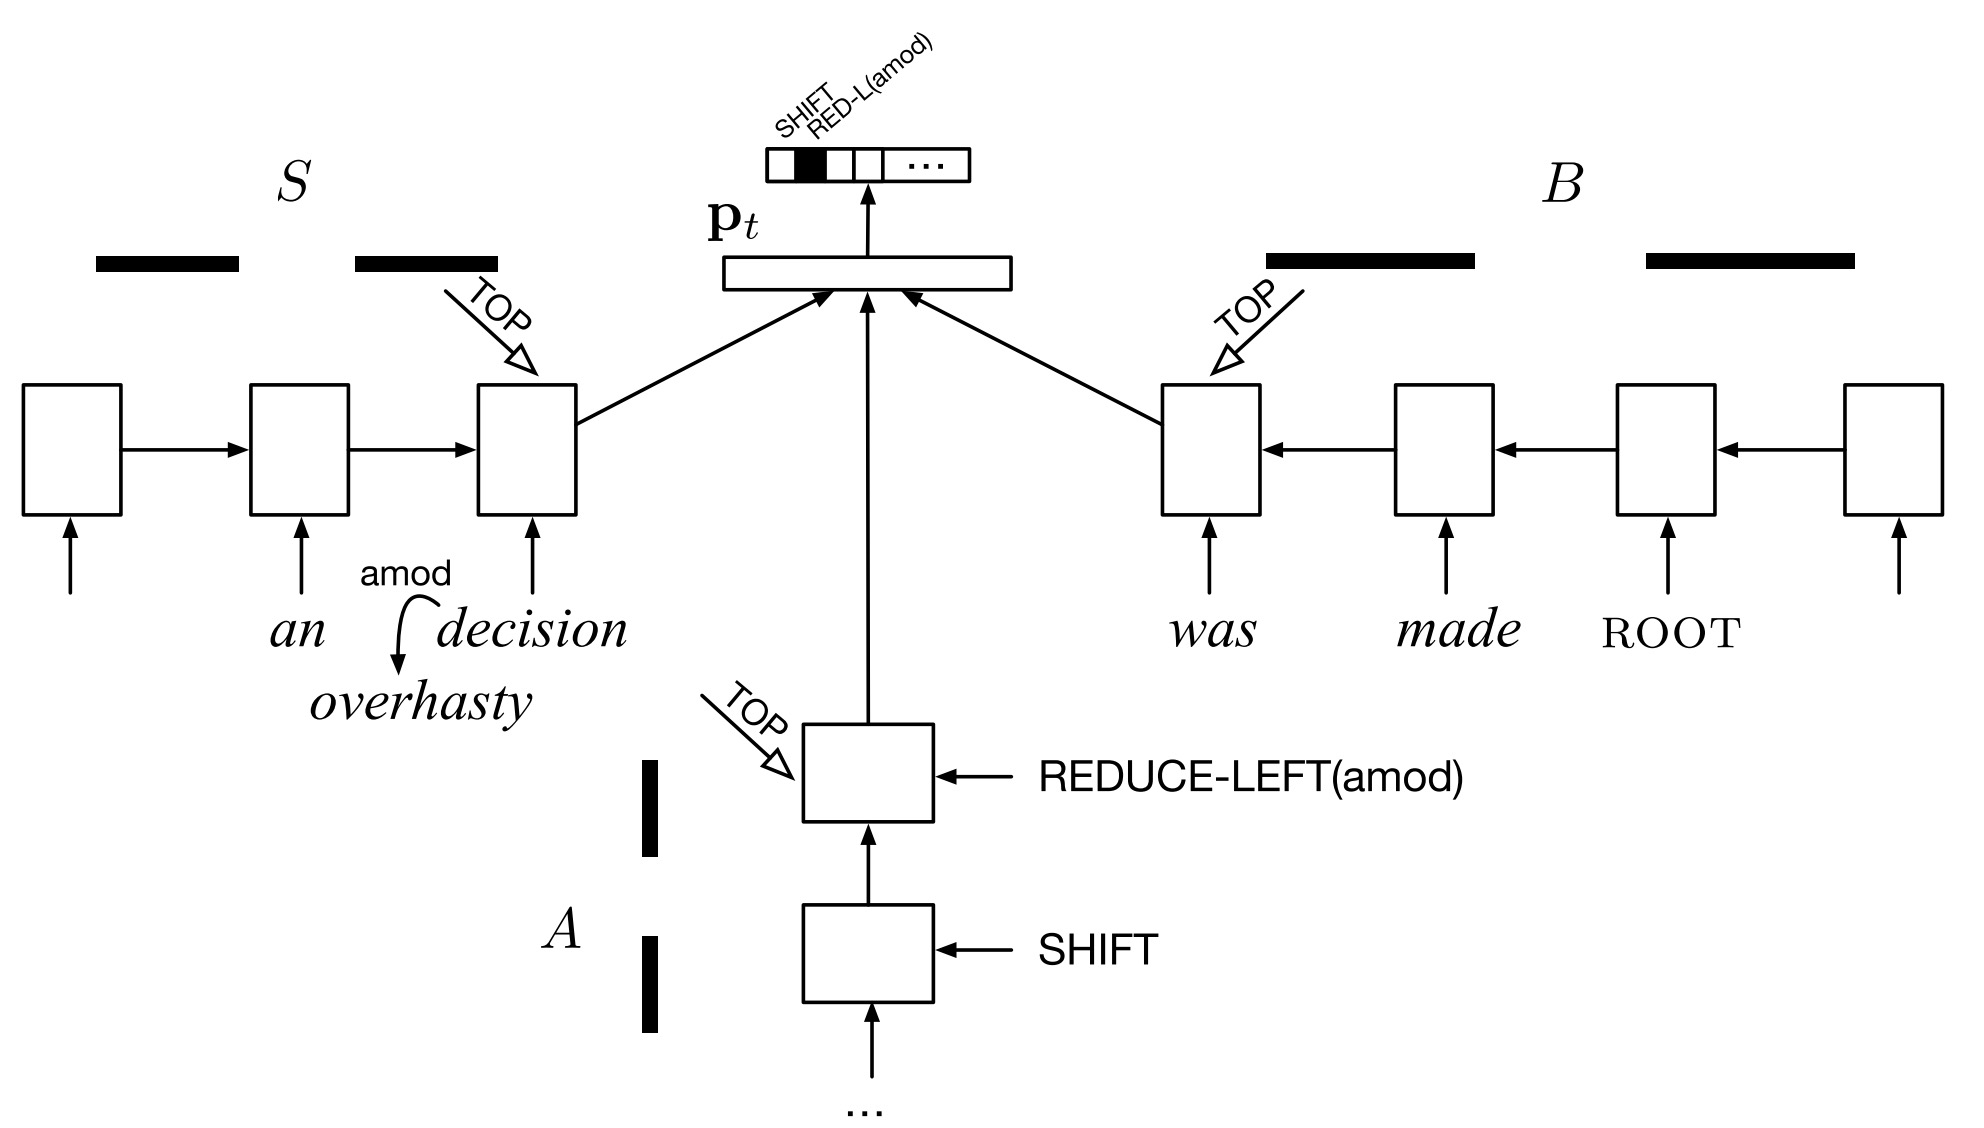
\includegraphics[width=0.8\columnwidth]{distill/dyer}}
	\subfigure{
		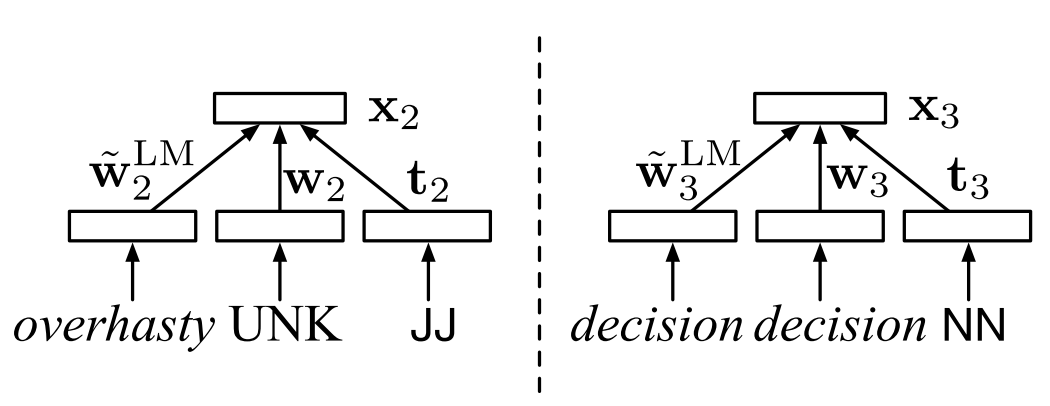
\includegraphics[width=0.5\columnwidth]{distill/inputs}}
	\bicaption{}{文献\inlinecite{dyer-EtAl:2015:ACL-IJCNLP}
		提出的基于转移的依存句法分析器。%左图为PTB实验结果,右图为IWSLT实验结果。
	}{Fig. $\!$}{The parser of Dyer et al. (2015) \inlinecite{dyer-EtAl:2015:ACL-IJCNLP}.
		\label{fig:parser}}
\end{figure}
本章在基于转移的句法分析中验证本章的知识蒸馏方法。
本章的参考文献\inlinecite{dyer-EtAl:2015:ACL-IJCNLP}
提出的stack-lstm parser构建本章的句法分析器。
其框架如图\ref{fig:parser}所示。
对于stack-lstm parser,
其输入词向量包括固定的词向量$\mathbf{p}$
与可调的词向量$\mathbf{w}$,其做法如图\ref{fig:parser}所示。
本章分别尝试对stack-lstm parser的集成模型以及基于上下文相关词向量的模型进行蒸馏。
通过对基于上下文相关词向量的模型进行蒸馏,
本章可以回答本章方法对教师模型与学生模型异构的情况下,
能否通过知识蒸馏的方式达到又快又好的结构预测的效果?

本章在此使用与第\ref{chp:seqlabel}章类似的方式
在基于转移的依存句法分析中加入上下文相关词向量。
即将其各层取平均,作为一种额外的固定的向量表示。
本章待蒸馏的模型则不含有对应的上下文相关词向量。
在这一节,本章使用的蒸馏过程与前文从两种状态中蒸馏的方法相同。

\section{实验}[Experiments]\label{sec:distill:vani-exp}
本章在
%两项任务 --- 基于转移的依存句法分析以及神经机器翻译上
基于转移的依存句法分析进行实验。
本章依据第\ref{sec:distill:sbsp}节
提到的方法将
%两项任务
基于转移的句法分析
转化为基于搜索的结构预测问题。

在基于转移的句法分析的实验中,
本章使用Dyer等人在2015年的文献\inlinecite{dyer-EtAl:2015:ACL-IJCNLP}
中提出的stack-lstm算法建模策略的分类器。\footnote{本章将句法分析代码开源在\url{https://github.com/Oneplus/twpipe}。}
%在神经网络机器翻译的实验中,
%本章使用基于注意力机制的编码器-解码器框架\cite{luong-pham-manning:2015:EMNLP}
%建模策略的分类器。\footnote{本章基于OpenNMT \cite{klein-EtAl:2017:ACL-2017-System-Demonstrations}进行了机器翻译实验并将这部分
%	实验代码开源于\url{https://github.com/Oneplus/OpenNMT-py}。}
%有关模型细节可以参考原文。

\subsection{设置}[Settings]
%\subsubsection{基于转移的依存句法分析}[Transition-based Dependency Parsing]

本章在宾州树库(Penn Treebank,简称PTB,文献\inlinecite{Marcus93buildinga})
数据集上进行实验。
本章使用标准数据划分(2-21节用作训练集,22节用作开发集,23节用作测试集)。
本章参考文献\cite{dyer-EtAl:2015:ACL-IJCNLP}并使用斯坦福依存句法(Stanford dependencies)规范
将短语结构句法转化为依存句法。\footnote{本章使用Stanford CoreNLP 3.3.0 (\url{https://stanfordnlp.github.io/CoreNLP/history.html})完成这一转化。}
本章通过10-折交叉验证获得训练数据的自动词性,其准确率为97.5\%。
本章使用不考虑标点符号的带标签依存关系准确率(LAS)评估通用依赖性分析性能。
本章的模型的超参数参考文献\inlinecite{dyer-EtAl:2015:ACL-IJCNLP}。
最好的迭代轮次由开发集性能决定。

文献\inlinecite{reimers-gurevych:2017:EMNLP2017}
指出神经网络的学习过程是非确定的,所以
汇报单次运行的结果并不能反映模型的性能。
为了消除随机初始化对模型性能的影响,
本章报告了20次随机运行的结果的平均值。

%\subsubsection{神经机器翻译}[Neural Machine Translation]
%\begin{figure}[t]
%	\centering
%	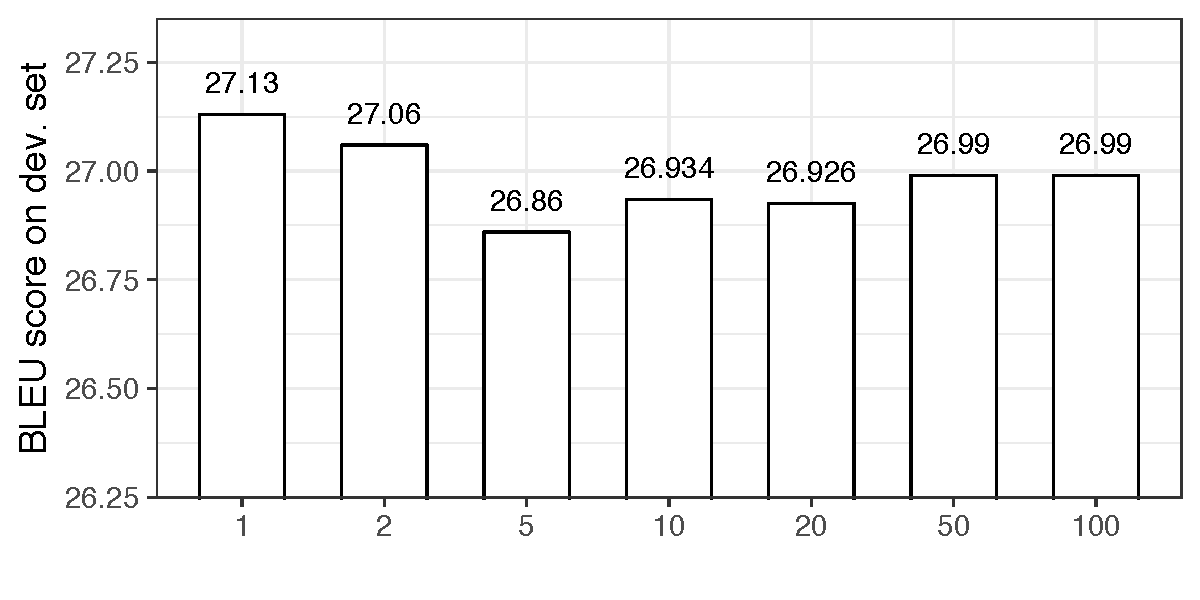
\includegraphics[width=0.7\columnwidth]{distill/approx}
%	\bicaption{}{使用的不同的概率$K$-最大输出对分布进行近似时的机器翻译的效果。}
%	{Fig. $\!$}{The effect of using different $K$s when approximating
%		distillation loss with $K$-most probable actions in the machine translation experiments.\label{fig:distill:approx}}
%\end{figure}
%
%本章在一个IWSLT2014德-英机器翻译数据集上进行实验。
%IWSLT2014德-英机器翻译数据集包含15.3万句训练数据,
%7千句开发集数据,以及7千句测试集数据。
%本章按照文献\inlinecite{DBLP:journals/corr/RanzatoCAZ15}
%建议的方法对数据进行预处理,
%并使用一个包含3万德语词以及2.5万英语词的词表作为模型的词表。
%本章参考文献\inlinecite{wiseman-rush:2016:EMNLP2016}
%并使用含有256个隐层单元的LSTM作为编码器与解码器。
%本章使用BLEU\cite{papineni-EtAl:2002:ACL}评价机器翻译的
%性能。\footnote{本章使用{\tt multi-bleu.perl}脚本评价机器翻译的性能。}
%与依存句法分析实验类似,
%本章汇报10次不同初始化条件下机器翻译模型的平均准确率。
%
%优化公式\ref{eq:distill:distill}需要枚举所有可能的动作。
%在神经机器翻译的情景下,由于词表非常大,
%这种枚举往往是非常耗时耗力的。
%为了使这种枚举可计算,本章使用根据
%集成模型得到的$K$个最可能动作作为
%整个$q(a\mid s)$概率分布的一种近似,
%即优化
%$\sum_a q(a \mid s) \cdot \log p(a \mid s) \approx
%\sum_k^K q(\hat{a}_k \mid s) \cdot \log p(\hat{a}_k \mid s)$学习目标。
%其中$\hat{a}_k$,是第$k$可能的动作。
%为了研究$K$的近似能力,本章将$\alpha$固定为1,
%通过调整$K$观察模型蒸馏的效果。
%图\ref{fig:distill:approx}显示了这一结果。
%从图\ref{fig:distill:approx}可见,$K$的不同并未带来显著的模型差异。
%故出于速度考虑,本章在后续实验中设定$K$为1。

\subsection{结果}[Results]\label{sec:distill:exp-res}

%\subsubsection{基于转移的依存句法分析}[Transition-based Dependency Parsing]
\begin{table}[t]
	\bicaption{}{句法分析的结果。
	显著性检验证明基于知识蒸馏的方法相对基线系统的提升以$p\le 0.01$
	统计显著。}{Table$\!$}{The dependency parsing results. 
		Significance test \cite{NILSSON08.52} shows the improvement of our \textit{Distill (both)} over \textit{Baseline}
		is statistically significant with $p<0.01$.\label{tbl:distill:parse-res}}
	\vspace{0.5em}\centering\wuhao
	\begin{tabular}{lc}
		\toprule[1.5pt]
		& LAS \\
		\midrule[1pt]
		Baseline & 90.83  \\
		Ensemble (20) & 92.73 \\
		Distill (reference, $\alpha$=1.0) & 91.99 \\
		Distill (exploration, $T$=1.0) & 92.00 \\
		Distill (both) & 92.14 \\
		\midrule[0.5pt]
		Ballesteros等人,文献\inlinecite{ballesteros-EtAl:2016:EMNLP2016}  (dyn. oracle) & 91.42 \\
		Andor等人,文献\inlinecite{andor-EtAl:2016:P16-1} (local, B=1) & 91.02 \\
		\midrule[0.5pt]
		Buckman等人,文献\inlinecite{buckman-ballesteros-dyer:2016:EMNLP2016} (local, B=8) & 91.19 \\
		Andor等人,文献\inlinecite{andor-EtAl:2016:P16-1} (local, B=32) & 91.70 \\
		Andor等人,文献\inlinecite{andor-EtAl:2016:P16-1} (global, B=32) & 92.79 \\
		Dozat与Manning,文献\inlinecite{DBLP:journals/corr/DozatM16} & 94.08 \\
		Kuncoro等人,文献\inlinecite{kuncoro-16} & 92.06 \\
		Kuncoro等人,文献\inlinecite{kuncoro-17} & 94.60 \\
		\bottomrule[1.5pt]
	\end{tabular}
\end{table}

\begin{table}[t]
	\bicaption{}{针对基于上下文相关词向量的句法分析的知识蒸馏实验。}
	{Table $\!$}{Distillation from structured prediction model with contextualized embeddings.\label{tbl:elmo-tb-parser}}
	\vspace{0.5em}\centering\wuhao
	\begin{tabular}{lcc}
		\toprule[1.5pt]
		model & LAS & spd. \\
		\midrule[1pt]
		Baseline & 90.83 & 1x \\
		\quad +ELMo & 92.64 & 7.3x \\
%		\quad +ELMo (ensemble 10) & 93.52 & 73x \\
		Distill (both) & 91.80 & 1x \\
		\bottomrule[1.5pt]
	\end{tabular}
\end{table}

表\ref{tbl:distill:parse-res}显示了PTB数据集上的实验结果。
这一结果显示集成模型高于基线模型1.90。
在将$\alpha$设置为1时,模型取得了最佳的开发集结果。
而此时测试集的准确率为91.99。

本章也研究了温度对于从探索状态中蒸馏的模型的影响。
图\ref{fig:distill:temperature}显示了这一结果。
根据表\ref{fig:distill:temperature},
在采样时使用尖锐的分布总体上取得了更好的开发集性能。
从探索状态蒸馏与从参考状态中蒸馏获得的模型的性能基本相当。
将两者结合进一步提高了准确率(带标签的依存关系准确率达到92.14)。

本章也在表\ref{tbl:distill:parse-res}中
将本章提出的模型与其他依存句法分析器进行了对比。
表\ref{tbl:distill:parse-res}的第二组显示了前人工作中
基于贪心解码的依存句法分析器的性能。
文献\inlinecite{andor-EtAl:2016:P16-1}
使用了与本章不同的状态表示方法,
同时分别研究了贪心解码与柱搜索(beam-search)的效果。
文献\inlinecite{ballesteros-EtAl:2016:EMNLP2016}
研究了使用dynamic oracle训练贪心解码的句法分析器
的问题。
本章提出的基于知识蒸馏的句法分析器的表现
好于这些基于贪心解码的句法分析器。
表\ref{tbl:distill:parse-res}显示了
其他依存句法分析算法的效果。
这些算法包括:在基于转移的句法分析中
使用柱搜索\cite{buckman-ballesteros-dyer:2016:EMNLP2016,andor-EtAl:2016:P16-1},
使用全局优化目标训练基于转移的依存句法分析\cite{andor-EtAl:2016:P16-1},
基于图的依存句法分析\cite{DBLP:journals/corr/DozatM16},
将基于图的依存句法分析器蒸馏到基于转移的依存句法分析器\cite{kuncoro-16},
以及将短语结构句法的结果通过规则转化为依存句法\cite{kuncoro-17}。
本章提出的基于知识蒸馏的方法由于这些基于转移的算法,
但相较其他算法仍有差距。
这类差距主要是由对问题的建模方式的不同导致的。

除了对集成模型进行蒸馏,
本章也尝试对基于上下文相关词向量的句法分析器进行蒸馏。
其实验结果如表\ref{tbl:elmo-tb-parser}所示。
根据表\ref{tbl:elmo-tb-parser},
使用本章提出的知识蒸馏方法可以从异构模型中有效地学习模型。
从而使用简单模型达到与使用上下文相关词向量模型类似的性能。
由于本章简单模型不使用上下文相关词向量,
所以,这一方法显著优化了模型速度。

%
%\subsubsection{神经机器翻译}[Neural Machine Translation]
%
%\begin{table}[t]
%	\bicaption{}{神经机器翻译的结果。
%		MIX代表文献\inlinecite{DBLP:journals/corr/RanzatoCAZ15}提出的基于强化学习的算法。
%		BSO代表文献\inlinecite{wiseman-rush:2016:EMNLP2016}提出的基于全局学习的算法。
%		显著性检验\cite{koehn:2004:EMNLP}证明基于知识蒸馏的方法相对基线系统的提升以$p\le 0.01$
%		统计显著。
%	}{Table$\!$}{The machine translation results.
%		MIXER denotes that of \inlinecite{DBLP:journals/corr/RanzatoCAZ15},
%		BSO  denotes that of \inlinecite{wiseman-rush:2016:EMNLP2016}.
%		Significance test \cite{koehn:2004:EMNLP} shows the improvement of our \textit{Distill (both)} over \textit{Baseline}
%		is statistically significant with $p<0.01$.\label{tbl:distill:nmt-res}}
%	\vspace{0.5em}\centering\wuhao
%	\begin{tabular}{lc}
%		\toprule[1.5pt]
%		& BLEU \\
%		\midrule[1pt]
%		Baseline & 22.79 \\
%		Ensemble (10) & 26.26 \\
%		Distill (reference, $\alpha$=0.8) & 24.76 \\
%		Distill (exploration, $T$=0.1) & 24.64 \\
%		Distill (both) & 25.44 \\
%		\midrule[0.5pt]
%		MIXER & 20.73 \\
%		BSO (local, B=1) & 22.53 \\
%		BSO (global, B=1) & 23.83 \\
%		\bottomrule[1.5pt]
%	\end{tabular}
%\end{table}
%
\begin{figure}[t]
	\centering
	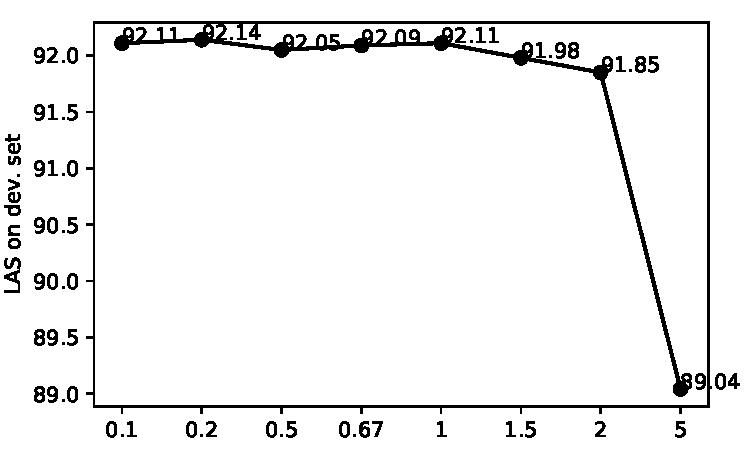
\includegraphics[width=0.6\textwidth]{distill/temperature}
	\bicaption{}{温度参数$T$对模型性能的影响。
		%左图显示的是句法分析的结果,右图显示的机器翻译的结果。
	}{Fig. $\!$}{The effect of $T$ on %PTB (left)
		%and IWSLT 2014 (right) 
		development set.\label{fig:distill:temperature}
	}
\end{figure}
%
%表\ref{tbl:distill:nmt-res}显示了IWSLT 2014数据集的机器翻译结果。
%与PTB的结果类似的是,对10个模型进行集成的效果超过
%基线系统3.47个BLEU值。
%从参考状态中进行知识蒸馏能够获得BLEU值为24.76的单模型。
%
%与基于转移的句法分析实验类似的是,
%在采样过程中尖锐的分布带来的模型的效果更好,
%然而,根据图\ref{fig:distill:temperature},
%在$T\le0.2$的情况下,$T$的不同导致的差异并不明显。
%在后续实验中,本章根据开发集结果设定$T=0.1$。
%表\ref{tbl:distill:nmt-res}显示从探索状态中进行知识蒸馏的
%模型获得24.64的准确率。
%这一准确率相机从参考状态中蒸馏有微小的差异。
%但将从参考中蒸馏和从探索中蒸馏进一步大幅度提高了准确率,
%并且获得了25.44的BLEU值。
%
%本章也将本章的模型与前人工作进行对比:
%对比的系统包括基于强化学习的机器翻译\cite{DBLP:journals/corr/RanzatoCAZ15},
%以及在翻译器学习过程中加入柱搜索\cite{wiseman-rush:2016:EMNLP2016}。
%对比显示本章提出的模型取得了最优的结果。
%
%上述句法分析与机器翻译实验
%表明仅从探索状态中进行知识蒸馏是可行的。
%同时将从参考状态中蒸馏与从探索状态中蒸馏进行结合可以进一步提高模型
%性能,并取得超越其他贪心搜索模型的性能。

%\paragraph{Speed Comparison}
%
%\begin{table}
%	\centering
%	\begin{tabular}{rrcc}
%		\hline
%		model & beam & BLEU & speed \\
%		Baseline & 1 & & \\
%		& 5 & & \\
%		& 10 & & \\
%		\hline
%		Distill both & & & \\
%		\hline
%	\end{tabular}
%\caption{Speed comparison.}
%\end{table}
%
%Beam search generally improves search-based structured predictor's perform
%according to previous literals \cite{buckman-ballesteros-dyer:2016:EMNLP2016,wiseman-rush:2016:EMNLP2016}.
%We run a beam-search decoding on the baseline model.

\subsection{分析}[Analysis]\label{sec:analysis}

根据第\ref{sec:distill:exp-res}节的结果,
使用集成模型显著提高了依存句法分析以及神经机器翻译的性能够。
然而,类似``为什么集成模型如此有效?
能不能放弃传统对数似然学习目标,完全从知识蒸馏学习目标中学习?
以及从知识蒸馏中学习是不是稳定的?''一类的问题并没有得到很好的回答。
在这一节中,
本章首先研究集成模型在``错误状态''上的表现
证明其具有更好的泛化能力。
然后,本章通过研究公式\ref{eq:distill:distill}中的$a$的作用
经验性地证明了完全从知识蒸馏中学习的可行性。
最后,本章通过分析表明知识蒸馏可以带来更稳定的模型学习。

\subsubsection{模型集成对于``错误状态''的作用}[Ensemble on ``Problematic'' States]\label{sec:distill:ens-on-states}
\begin{table}[t]
	\bicaption{}{不同模型的``错误状态''的排序性能。}{Table $\!$}{The ranking performance of parsers' 
		output distributions evaluated in MAP on
		``problematic'' states.\label{tbl:state-ana}}
	\vspace{0.5em}\centering\wuhao
	\begin{tabular}{l  c c}
		\toprule[1.5pt]
		& 有歧义的正确状态 & 非正确状态 \\
		\midrule[1pt]
		Baseline & 68.59 & 89.59\\
		Ensemble & 74.19 & 90.90 \\
		Distill (both) & 81.15 & 91.38 \\
		\bottomrule[1.5pt]
	\end{tabular}
\end{table}
如前文所述,歧义或者非最优的``错误状态''影响结构预测的准确率。
根据第\ref{sec:distill:exp-res}节的结果,模型集成能够提升性能,
这表明其能够更好地处理``错误状态''。
为了经验性地验证这一假设,
本章以依存句法分析为目标,
借助dynamic oracle研究集成模型的输出分布。

dynamic oracle\cite{goldberg-nivre:2012:PAPERS,TACL302} 
能够有效地判断,对于一棵句法树的任意给定状态$s$,
最优的转移动作(\textit{参考动作})是什么。
这里``最优''指的是能够搜索得到的相似度(用LAS衡量)最高的树。
这种性质使得本章可以对``错误状态''中的某个动作进行分析。
本章根据\textit{参考动作}
评价了基线模型以及集成模型在动作空间上输出的分布。
由于dynamic oracle会对一个状态给出多个参考动作,
本章将这一评价问题转化为一个排序的评价问题。
直观来讲,当多个参考动作存在是,
一个好的句法分析器应当将动作的概率密度集中在参考动作上。
本章通过随机采样从基线模型中获得了一系列状态。
不同模型的排序分数如表\ref{tbl:state-ana}所示。
根据表\ref{tbl:state-ana},
集成模型在``错误状态''下的排序表现更好。
这一观察表明,集成模型的输出分布所包含的信息更丰富,
因而在``错误状态''上表现得更好,并取得更好的性能。
同时,本章也观察到蒸馏模型的性能好于基线与集成模型。
本章认为造成这一现象的原因是蒸馏模型的学习过程包含探索机制。

\subsubsection{$\alpha$的效果}[Effect of $\alpha$]
\begin{figure}[t]
	\centering
	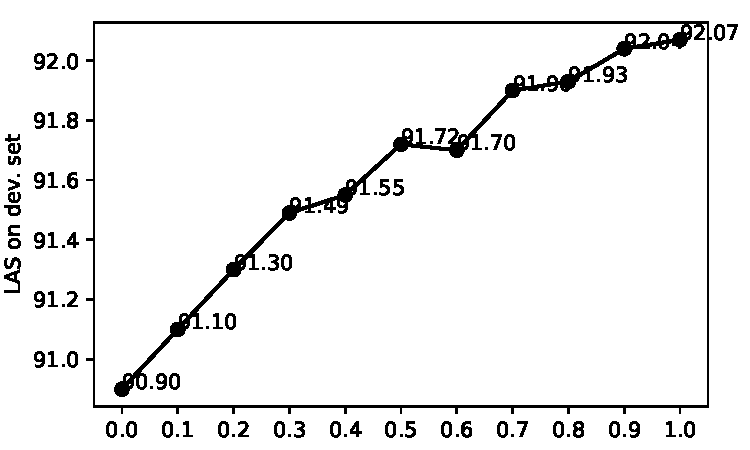
\includegraphics[width=0.6\columnwidth]{distill/alpha}
	\bicaption{}{开发集上$\alpha$值的效果%左图为PTB实验结果,右图为IWSLT实验结果。
	}{Fig. $\!$}{The effect of $\alpha$% on PTB (left)
		%and IWSLT 2014 (right) development set.
		\label{fig:alpha}}
\end{figure}

本章在从参考状态中蒸馏模型的学习过程中研究$\alpha$的影响。
本章在基于转移的句法分析以及神经机器翻译中将$\alpha$从0到1以0.1为步长变化,
并在图\ref{fig:alpha}中展示了模型的性能。
两个实验都显示大$\alpha$的表现好于小$\alpha$。
对于句法分析,$\alpha=1$时取得了最好的开发集性能。
对于神经机器翻译,开发集性能最好的$\alpha$是0.8。
同时,在机器翻译实验中,$\alpha=0.8$与$\alpha=1$的模型只有0.2的差距。
这一系列观察表明对于从参考状态时,
更多地关注知识蒸馏的学习目标能够带来更好的模型性。
这一观察也显示对于从探索状态中蒸馏模型(即$\alpha=1$)
的可行性。

\subsubsection{模型学习的稳定性}[Learning Stability]
\begin{figure}[t]
	\centering
	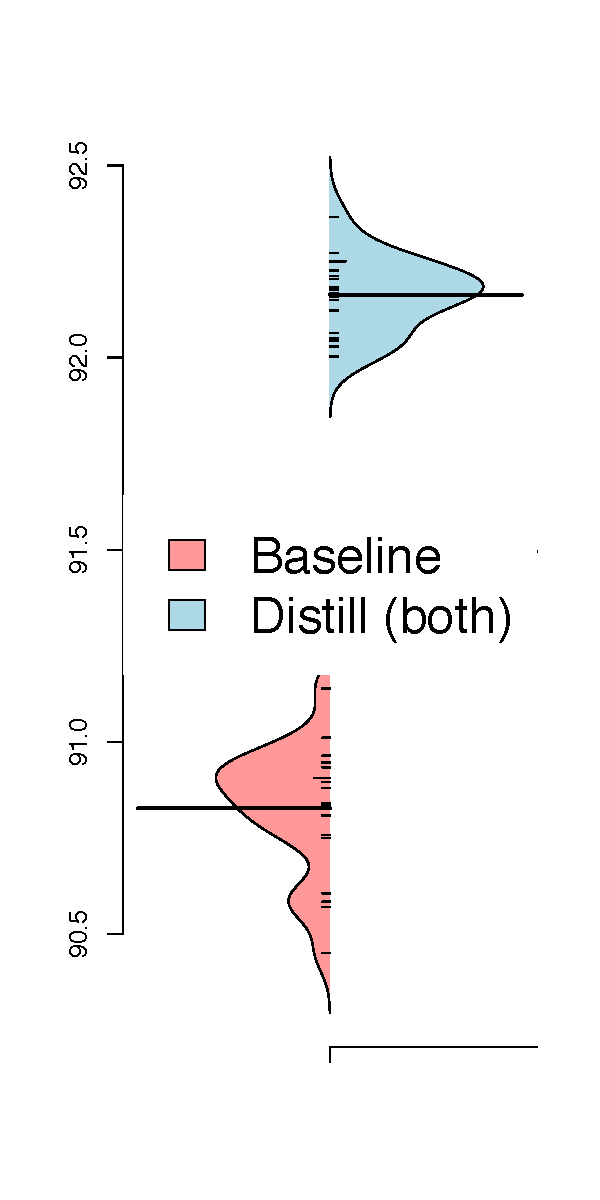
\includegraphics[width=0.3\columnwidth, trim={0, 1cm, 0, 1.5cm}, clip]{distill/stability_par_bean}
%	\subfigure{\includegraphics[width=0.3\columnwidth, trim={0, 1cm, 0, 1.5cm}, clip]{distill/stability_nmt_bean}}
	\bicaption{}{不同随机种子下模型分数的分布。
		%左图显示PTB上测试集的结果,右图显示IWSLT上测试集的结果。
	}{Fig. $\!$}{The distributions of scores for the baseline model and
		our {\it distillation from both} on PTB
		% test (left) and IWSLT 2014 test (right)
		on differently-seeded runs.\label{fig:stable}}
\end{figure}

\begin{table}[t]
	\bicaption{}{结果的最大值、最小值以及标准差。}{Table $\!$}{The minimal, maximum, and standard derivation values
		on differently-seeded runs.\label{tbl:stable}}
	\vspace{0.5em}\centering\wuhao
	\begin{tabular}{rcccc}
		\toprule[1.5pt]
		system & seeds & min & max & $\sigma$ \\
		\midrule[1pt]
		\multicolumn{2}{r}{\it PTB test} & & & \\
		Baseline & 20 & 90.45 & 91.14 & 0.17 \\
		Distill (both) & 20 & 92.00 & 92.37 & 0.09 \\
%		\midrule[0.5pt]
%		\midrule[0.5pt]
%		\multicolumn{2}{r}{\it IWSLT 2014 test} & & & \\
%		Baseline & 10 & 21.63 & 23.67 & 0.55 \\
%		Distill (both) & 10 & 24.22 & 25.65 & 0.12 \\
		\bottomrule[1.5pt]
	\end{tabular}
\end{table}
除了提高性能,
知识蒸馏也能给模型学习的稳定性带来提升。
本章将不同随机种子得到的基线模型与蒸馏模型的准确率
以琴图的方式绘制在图\ref{fig:stable}中,
同时在表\ref{tbl:stable}中显示了两种模型的标准差。
可见,知识蒸馏模型的标准差更小,
即其学习更稳定。
文献\inlinecite{DBLP:journals/corr/KeskarMNST16}指出
影响神经网络模型的泛化性能的主要问题并非过拟合,
而是模型参数进入尖锐的局部极小点(sharp minimizer)。
这种局部极小点的泛化性往往较差。
根据这一理论,本章猜测知识蒸馏取得更稳定的训练效果的原因是
知识蒸馏的学习曲目更光滑,尖锐的局部极小点更少。

\section{相关工作}[Related Work]

前人工作中有若干在NLP任务中使用知识蒸馏技术。
Kim与Rush在2016年的文献\inlinecite{kim-rush:2016:EMNLP2016}
中关注如将复杂模型蒸馏到简单模型中。
同时,他们的方法主要关注序列级别的蒸馏。
与之相反的是,本章更关注动作级的知识蒸馏,
同时提出从参考状态以及从探索状态中进行知识蒸馏。

Freitag等人在2017年的文献\inlinecite{DBLP:journals/corr/FreitagAS17}
中使用六个翻译器的译文生成翻译的训练数据,
其模型使用柱搜索进行探索。
与其不同的是,
本章使用单模型产生训练数据,并以拟合集成模型的分布为学习目标。

在强化学习中,
集成模型的探索机制也得到了相应的研究\cite{NIPS2016_6501}。
除了在标注数据上蒸馏模型,
也有一部分半监督学习的工作从生语料上进行模型学习\cite{liang:icml08,li-zhang-chen:2014:P14-1}。
如何在生语料上进行知识蒸馏也值得后续工作的研究。

Kuncoro在2016年的文献\inlinecite{kuncoro-16}
中提出将20个基于转移的句法分析器的结果通过投票的方式进行集成并
将结果以后验正则的方式应用于训练一个基于图的模型。
不同于他们的模型,将基于转移的模型蒸馏到基于转移的模型中。

除了使用知识蒸馏,
Stahlberg等人在2017年的文献\inlinecite{stahlberg-byrne:2017:EMNLP2017}
中提出将若干翻译模型的集成组合为一个神经网络,并用SVD化简了模型。
他们的模型也可以视作一种知识蒸馏。

\section{本章小结}[Conclusion]
本章研究了结构预测中的知识蒸馏问题。
本章提出将若干模型的模型集成蒸馏到一个单模型中。
这一蒸馏过程同时在参考状态以及探索状态中完成。
在基于转移的句法分析
%以及神经机器翻译
实验中,
本章模型获得了显著的性能提升,从而证明了本章提出的方法的有效性。
同时,本章通过分析给出了本章知识蒸馏方法可行性的验证。

在此基础上,
本章对于基于上下文相关词向量的句法分析器进行知识蒸馏。
实验结果显示本章提出的方法对于异构模型同样有效,
在少量损失精度的情况下近十倍地提高模型速度。
\backmatter
%硕博书序
% !Mode:: "TeX:UTF-8" 
\begin{conclusions}

包括分词、词性标注、命名实体识别以及句法分析在内的
语言分析是基础而重要的自然语言处理问题。
提高语言分析的性能能够有效地帮助下游任务。
强化词表示能力是提高语言分析性能的一种有效手段。
近年来提出的上下文相关词向量已经帮助一部分自然语言处理任务
取得了性能提升。
本文受到相关研究的启发,
针对上下文相关词向量与语言分析的结合开展了一系列研究。

本文针对现有上下文相关词向量因过分强调使用多层网络对
一整句甚至多句进行抽象而导致的效率问题,
从语言分析主要依赖局部信息出发,
提出一种融合相对位置权重的窗口级自注意力机制
并将其应用于上下文表示,从而获得一种适用于语言分析的上下文相关词向量。
本文在五项语言分析任务上进行实验,
相应结果表明本文提出的上下文相关词向量在
不损失精度的情况下获得了三倍的速度提升。

基于前文提出的上下文相关词向量,
本文针对语言分析中的切分问题(中文分词与命名实体识别)
对合理的片段(词与实体)表示的依赖,
本文在上下文相关词向量的基础上
提出一种基于简单拼接的片段表示方法并
将其应用于半-马尔科夫条件随机场中。
在典型切分问题的实验中,
本文基于上下文相关词向量的片段表示有效地提高了模型性能。
通过进一步融合任务相关的上下文表示以及
建模片段级信息的片段向量,本文模型取得了当前最优的性能。

基于前文提出的上下文相关词向量,
本文针对上下文相关词向量对多国语句法分析作用尚无明确结论的现状,
提出在多国语句法分析中使用上下文相关词向量
并在大规模树库上验证上下文相关词向量的有效性。
除了获得稳定且显著的性能提升,
本文针对提升的原因进行了详细的分析。
大量分析实验表明,
性能提升的主要原因是上下文相关词向量
通过对于未登录词词形的更好的建模
有效地提升了未登录词的准确率。

针对使用上下文相关词向量的句法分析参数过多、运行速度较慢的问题,
本文提出一种结合探索机制的知识蒸馏算法,
以将基于上下文相关词向量的复杂模型
用不使用相应词向量的简单模型进行近似,
从而在不显著降低性能的情况下提高句法分析速度。
实验结果表明,
本文提出的方法
在损失少量句法分析准确率的情况下,
近十倍地提升了速度。

本文研究表明上下文相关词向量可以很好地与语法分析结合,
从而显著提高语法分析的性能。
同时,本文也以语言分析为工具
对于上下文相关词向量进行全面的分析。
这些分析表明上下文相关词向量具有表示未登录词,
建模片段的能力。
%学位论文的结论作为论文正文的最后一章单独排写,但不加章标题序号。
%
%结论应是作者在学位论文研究过程中所取得的创新性成果的概要总结,不能与摘要混为一谈。博士学位论文结论应包括论文的主要结果、创新点、展望三部分,在结论中应概括论文的核心观点,明确、客观地指出本研究内容的创新性成果(含新见解、新观点、方法创新、技术创新、理论创新),并指出今后进一步在本研究方向进行研究工作的展望与设想。对所取得的创新性成果应注意从定性和定量两方面给出科学、准确的评价,分(1)、(2)、(3)…条列出,宜用“提出了”、“建立了”等词叙述。

\end{conclusions}
   % 结论
\bibliographystyle{hithesis} %如果没有参考文献时候
\bibliography{tinydb}
%\begin{appendix}%附录
%\input{back/appA.tex}
%\end{appendix}
% !Mode:: "TeX:UTF-8" 

\begin{publication}
\noindent\textbf{(一)发表的学术论文}
\begin{publist}
\item \textbf{Yijia Liu}, Wanxiang Che, Huaipeng Zhao, Bing Qin, and Ting Liu. Distilling Knowledge for Search-based Structured Prediction[C]// Proceedings of the 56th Annual Meeting of the Association for Computational Linguistics (ACL,CCF~A类会议)
\item \textbf{Yijia Liu}, Wanxiang Che, Jiang Guo, Bing Qin, and Ting Liu. Exploring Segment Representations for Neural Segmentation Models[C]// Proceedings of 25th International Joint Conference on Artificial Intelligence(IJCAI,CCF~A类会议)
\item \textbf{Yijia Liu}, Wanxiang Che, Bing Qin, and Ting Liu. HC-search for Incremental Parsing[C]// Proceedings of 25th International Joint Conference on Artificial Intelligence(IJCAI,CCF~A类会议)
\item \textbf{Yijia Liu}, Wanxiang Che, Bo Zheng, Bing Qin, and Ting Liu.  An AMR Aligner Tuned by Transition-based Parser[C]// Proceedings of the 2018 Conference on Empirical Methods in Natural Language Processing(EMNLP,CCF~B类会议)
\item \textbf{Yijia Liu}, Yue Zhang, Wanxiang Che, and Ting Liu. Domain Adaptation for CRF-based Chinese Word Segmentation using Free Annotations[C]// Proceedings of the 2014 Conference on Empirical Methods in Natural Language Processing (EMNLP,CCF~B类会议)
\item \textbf{Yijia Liu}, Yi Zhu, Wanxiang Che, Bing Qin, Nathan Schneider, and Noah A. Smith. Parsing Tweets into Universal Dependency[C]// Proceedings of the 2018 Conference of the North American Chapter of the Association for Computational Linguistics: Human Language Technologies (NAACL,CCF~C类会议)
\item \textbf{Yijia Liu}, Yue Zhang, Wanxiang Che, and Ting Liu. Transition-Based Syntactic Linearization[C]// Proceedings of the 2015 Conference of the North American Chapter of the Association for Computational Linguistics: Human Language Technologies (NAACL,CCF~C类会议)
\item \textbf{Yijia Liu}, Wanxiang Che, Yuxuan Wang, Bo Zheng, Yanyan Zhao, Bing Qin and Ting Liu. Deep contextualized word embeddings on universal dependency parsing[J]//
\item Yutai Hou, \textbf{Yijia Liu}, Wanxiang Che and Ting Liu, Sequence-to-Sequence Data Augmentation for Dialogue Language Understanding[C]// Proceedings of the 27th International Conference on Computational Linguistics (COLING,CCF~B类会议)
\item Haoyang Wen, \textbf{Yijia Liu}, Wanxiang Che, Libo Qin and Ting Liu, Sequence-to-Sequence Learning for Task-oriented Dialogue with Dialogue State Representation[C]// Proceedings of the 27th International Conference on Computational Linguistics (COLING,CCF~B类会议)
\end{publist}

\noindent\textbf{(二)申请及已获得的专利(无专利时此项不必列出)}
\begin{publist}
\item 车万翔、\textbf{刘一佳}、赵妍妍、刘挺.~一种中文分词增量学习方法:中国,CN201510604035.0[P]. 2015-11-18.
\end{publist}

\noindent\textbf{(三)参与的科研项目及获奖情况}
\begin{publist}
\item 刘挺、车万翔、胡郁、秦兵、陈毅恒、胡国平、张宇、赵妍妍、马汉君、张伟男、\textbf{刘一佳}.~语言技术平台及其应用. 黑江省科学技术一等奖, 2016.
\item Wanxiang Che, \textbf{Yijia Liu}, Yuxuan Wang, Bo Zheng, and Ting Liu. Towards Better UD Parsing: Deep Contextualized Word Embeddings, Ensemble, and Treebank Concatenation[C]// Proceedings of the CoNLL 2018 Shared Task: Multilingual Parsing from Raw Text to Universal Dependencies (CoNLL 2018通用多国语依存句法分析评测,LAS第一)
\end{publist}
%\vfill
%\hangafter=1\hangindent=2em\noindent
%\setlength{\parindent}{2em}
\end{publication}
    % 所发文章
\include{back/ceindex}    % 索引, 根据自己的情况添加或者不添加,选择自动添加或者手工添加。
\authorization %授权
%\authorization[saomiao.pdf] %添加扫描页的命令,与上互斥
% !Mode:: "TeX:UTF-8"
\begin{acknowledgements}

本文是在导师秦兵教授与副导师车万翔教授的共同指导下完成的。
没有两位老师对于文章内容的编排以及对于文章进度的督促,本文是无法在保证质量的情况下按时完成的。
同时,刘挺教授及其领导的哈工大社会计算与信息检索研究中心
也为本文的完成提供了充分的支持。
具体到文章内容,
本文第\ref{chp:semicrf}章内容得到了麻省理工学院的郭江研究员的指导与帮助。
本文第\ref{chp:seqlabel}章的实验是在王宇轩与郑博两位师弟的共同努力下完成的。
本文第\ref{chp:distill}章的实验是在赵怀鹏师弟的帮助下完成的。
除此之外,
天津大学的张梅山副教授对于本文第\ref{chp:seqlabel}章,
文灏洋师弟对于本文第\ref{chp:elmo}与\ref{chp:seqlabel}章
分别给出了宝贵的意见。
本文的完成与各位同仁的辛勤劳动是密不可分的。

除了博士论文关注的内容,
本文作者博士期间的相关研究也得到了多位同仁的帮助指导。
其中包括苏州大学的李正华副教授、
西湖大学的张岳副教授、
美国华盛顿大学的Noah A. Smith副教授、
美国乔治华盛顿大学的Nathan Schneider助理教授、
剑桥大学的朱懿以及王少磊、侯宇泰、覃立波、文灏洋四位师弟。

自本文作者于2011年进入实验室开始科研工作,
导师秦兵教授给予本文作者多方面的关怀。
其中既有对科研的指导,也有对生活的鼓励。
这些指导与鼓励使本文作者感受到家的温暖,
更加地热爱这个集体。

自2008年考入哈工大计算机学院到2019年提交博士论文,
本文作者的成长过程也得到了副导师车万翔教授的巨大帮助。
2008年秋,车教授任教高级语言程序设计并给本文作者当年的唯一满分。
此事培养了本文作者对于计算机的兴趣与自信。
2011年,车教授介绍本文作者进入社会计算与信息检索研究中心开展科研工作,
并将实验室的重点项目 --- 语言技术平台的开发工作交付给本文作者,
使其对于语言分析技术有了深入的了解与认识。
2013年与2016年,车教授又分别推荐本文作者去新加坡、美国交流访学,
开阔了其研究思路与视野。

实验室主任刘挺教授也从多方面对本文作者进行了指导。
刘挺教授的言传身教塑造了本文作者的基本学术价值观。
同时,在本文作者开始科研工作之初,
刘挺教授强调的``一万小时''、``成为专家''
的观点都对本文作者产生了积极的影响。
刘挺教授也积极为包括本文作者在内的实验室成员创造学习交流机会。
在与毕业师兄交流中,本文作者学得的时间管理技术并受益良多。

2013年到2014年,本文作者访问新加坡科学与设计大学,
在张岳副教授的指导下进行了一年的科研工作。
这段访问经历从基本科研方法、论文写作等方面锻炼了本文作者,
对于本文作者的快速成长有重大意义。

2016年到2017年,本文作者访问美国华盛顿大学并得到Noah A. Smith教授的指导。
Smith教授帮助本文作者更好地理解了自然语言处理与机器学习之间的关系。
更重要的是,通过与Smith教授的交流,本文作者认识到学术合作的重要性。

本文作者也要感谢实验室的张宇教授,刘铭副教授,丁效老师以及冯骁骋老师。
几位老师在工作生活中对本文作者给出有效的建议。
同时,本文作者也要感谢包括牛国成、韩冰、徐伟、徐梓翔、刘洋等等共同奋斗的同学。

最后,本文作者需要感恩父母给予其生命,养育其成人,支持其完成博士学业。

%本文作者妄自感谢快速变革的时代。

\end{acknowledgements}
 %致谢
% !Mode:: "TeX:UTF-8" 

\begin{resume}
刘一佳,男,1988年8月,出生于辽宁省本溪市。

\textbf{教育经历}
\begin{itemize}
	\item 2012年9月至今:哈尔滨工业大学计算机学院社会计算与信息检索研究中心攻读工学博士学位,导师为秦兵教授,副导师为车万翔教授;
	\item 2012年9月 --- 2014年7月:哈尔滨工业大学计算机学院社会计算与信息检索研究中心获得工学硕士学位,导师为车万翔副教授;
	\item 2008年9月 --- 2012年7月:哈尔滨工业大学计算机学院获得工学学士学位。
\end{itemize}

\textbf{实习经历}
\begin{itemize}
	\item 2016年9月 --- 2017年9月:美国华盛顿大学(University of Washington),导师为Noah A. Smith副教授;
	\item 2013年10月 --- 2014年10月:新加坡科学与设计大学(Singapore University of Technology and Design)访问,导师
	为张岳助理教授;
	\item 2011年7月 --- 2011年11月:北京百度公司自然语言处理部门实习。
\end{itemize}

\textbf{获奖情况}

\begin{itemize}
	\item 2018年12月:百度奖学金;
	\item 2016年9月:华为奖学金(研究生阶段);
	\item 2013年9月:国家奖学金(研究生阶段);
	\item 2010年10月:2010年国际大学生程序设计竞赛亚洲区赛杭州站,银奖;
	\item 2010年9月:华为奖学金(本科阶段)。
\end{itemize}

\textbf{项目经历}

\begin{itemize}
	\item 2018年4月 --- 2018年6月:CoNLL 2018: 多语言通用依存分析评测;
	\item 2013年至今:语言技术平台。
\end{itemize}

\end{resume}
          % 博士学位论文有个人简介

%本科书序为:
%% !Mode:: "TeX:UTF-8" 
\begin{conclusions}

包括分词、词性标注、命名实体识别以及句法分析在内的
语言分析是基础而重要的自然语言处理问题。
提高语言分析的性能能够有效地帮助下游任务。
强化词表示能力是提高语言分析性能的一种有效手段。
近年来提出的上下文相关词向量已经帮助一部分自然语言处理任务
取得了性能提升。
本文受到相关研究的启发,
针对上下文相关词向量与语言分析的结合开展了一系列研究。

本文针对现有上下文相关词向量因过分强调使用多层网络对
一整句甚至多句进行抽象而导致的效率问题,
从语言分析主要依赖局部信息出发,
提出一种融合相对位置权重的窗口级自注意力机制
并将其应用于上下文表示,从而获得一种适用于语言分析的上下文相关词向量。
本文在五项语言分析任务上进行实验,
相应结果表明本文提出的上下文相关词向量在
不损失精度的情况下获得了三倍的速度提升。

基于前文提出的上下文相关词向量,
本文针对语言分析中的切分问题(中文分词与命名实体识别)
对合理的片段(词与实体)表示的依赖,
本文在上下文相关词向量的基础上
提出一种基于简单拼接的片段表示方法并
将其应用于半-马尔科夫条件随机场中。
在典型切分问题的实验中,
本文基于上下文相关词向量的片段表示有效地提高了模型性能。
通过进一步融合任务相关的上下文表示以及
建模片段级信息的片段向量,本文模型取得了当前最优的性能。

基于前文提出的上下文相关词向量,
本文针对上下文相关词向量对多国语句法分析作用尚无明确结论的现状,
提出在多国语句法分析中使用上下文相关词向量
并在大规模树库上验证上下文相关词向量的有效性。
除了获得稳定且显著的性能提升,
本文针对提升的原因进行了详细的分析。
大量分析实验表明,
性能提升的主要原因是上下文相关词向量
通过对于未登录词词形的更好的建模
有效地提升了未登录词的准确率。

针对使用上下文相关词向量的句法分析参数过多、运行速度较慢的问题,
本文提出一种结合探索机制的知识蒸馏算法,
以将基于上下文相关词向量的复杂模型
用不使用相应词向量的简单模型进行近似,
从而在不显著降低性能的情况下提高句法分析速度。
实验结果表明,
本文提出的方法
在损失少量句法分析准确率的情况下,
近十倍地提升了速度。

本文研究表明上下文相关词向量可以很好地与语法分析结合,
从而显著提高语法分析的性能。
同时,本文也以语言分析为工具
对于上下文相关词向量进行全面的分析。
这些分析表明上下文相关词向量具有表示未登录词,
建模片段的能力。
%学位论文的结论作为论文正文的最后一章单独排写,但不加章标题序号。
%
%结论应是作者在学位论文研究过程中所取得的创新性成果的概要总结,不能与摘要混为一谈。博士学位论文结论应包括论文的主要结果、创新点、展望三部分,在结论中应概括论文的核心观点,明确、客观地指出本研究内容的创新性成果(含新见解、新观点、方法创新、技术创新、理论创新),并指出今后进一步在本研究方向进行研究工作的展望与设想。对所取得的创新性成果应注意从定性和定量两方面给出科学、准确的评价,分(1)、(2)、(3)…条列出,宜用“提出了”、“建立了”等词叙述。

\end{conclusions}
   % 结论
%\bibliographystyle{hithesis}
%\bibliography{reference}
%\authorization %授权
%%\authorization[saomiao.pdf] %添加扫描页的命令,与上互斥
%% !Mode:: "TeX:UTF-8"
\begin{acknowledgements}

本文是在导师秦兵教授与副导师车万翔教授的共同指导下完成的。
没有两位老师对于文章内容的编排以及对于文章进度的督促,本文是无法在保证质量的情况下按时完成的。
同时,刘挺教授及其领导的哈工大社会计算与信息检索研究中心
也为本文的完成提供了充分的支持。
具体到文章内容,
本文第\ref{chp:semicrf}章内容得到了麻省理工学院的郭江研究员的指导与帮助。
本文第\ref{chp:seqlabel}章的实验是在王宇轩与郑博两位师弟的共同努力下完成的。
本文第\ref{chp:distill}章的实验是在赵怀鹏师弟的帮助下完成的。
除此之外,
天津大学的张梅山副教授对于本文第\ref{chp:seqlabel}章,
文灏洋师弟对于本文第\ref{chp:elmo}与\ref{chp:seqlabel}章
分别给出了宝贵的意见。
本文的完成与各位同仁的辛勤劳动是密不可分的。

除了博士论文关注的内容,
本文作者博士期间的相关研究也得到了多位同仁的帮助指导。
其中包括苏州大学的李正华副教授、
西湖大学的张岳副教授、
美国华盛顿大学的Noah A. Smith副教授、
美国乔治华盛顿大学的Nathan Schneider助理教授、
剑桥大学的朱懿以及王少磊、侯宇泰、覃立波、文灏洋四位师弟。

自本文作者于2011年进入实验室开始科研工作,
导师秦兵教授给予本文作者多方面的关怀。
其中既有对科研的指导,也有对生活的鼓励。
这些指导与鼓励使本文作者感受到家的温暖,
更加地热爱这个集体。

自2008年考入哈工大计算机学院到2019年提交博士论文,
本文作者的成长过程也得到了副导师车万翔教授的巨大帮助。
2008年秋,车教授任教高级语言程序设计并给本文作者当年的唯一满分。
此事培养了本文作者对于计算机的兴趣与自信。
2011年,车教授介绍本文作者进入社会计算与信息检索研究中心开展科研工作,
并将实验室的重点项目 --- 语言技术平台的开发工作交付给本文作者,
使其对于语言分析技术有了深入的了解与认识。
2013年与2016年,车教授又分别推荐本文作者去新加坡、美国交流访学,
开阔了其研究思路与视野。

实验室主任刘挺教授也从多方面对本文作者进行了指导。
刘挺教授的言传身教塑造了本文作者的基本学术价值观。
同时,在本文作者开始科研工作之初,
刘挺教授强调的``一万小时''、``成为专家''
的观点都对本文作者产生了积极的影响。
刘挺教授也积极为包括本文作者在内的实验室成员创造学习交流机会。
在与毕业师兄交流中,本文作者学得的时间管理技术并受益良多。

2013年到2014年,本文作者访问新加坡科学与设计大学,
在张岳副教授的指导下进行了一年的科研工作。
这段访问经历从基本科研方法、论文写作等方面锻炼了本文作者,
对于本文作者的快速成长有重大意义。

2016年到2017年,本文作者访问美国华盛顿大学并得到Noah A. Smith教授的指导。
Smith教授帮助本文作者更好地理解了自然语言处理与机器学习之间的关系。
更重要的是,通过与Smith教授的交流,本文作者认识到学术合作的重要性。

本文作者也要感谢实验室的张宇教授,刘铭副教授,丁效老师以及冯骁骋老师。
几位老师在工作生活中对本文作者给出有效的建议。
同时,本文作者也要感谢包括牛国成、韩冰、徐伟、徐梓翔、刘洋等等共同奋斗的同学。

最后,本文作者需要感恩父母给予其生命,养育其成人,支持其完成博士学业。

%本文作者妄自感谢快速变革的时代。

\end{acknowledgements}
 %致谢
%\begin{appendix}%附录
%\input{body/appendix01}%本科生翻译论文
%\end{appendix}

\end{document}
